% ******************************* PhD Thesis Template **************************
% Please have a look at the README.md file for info on how to use the template

\documentclass[a4paper,12pt,print,custombib,custommargin,openany, twoside]{Classes/PhDThesisPSnPDF}

% ******************************************************************************
% ******************************* Class Options ********************************
% *********************** See README for more details **************************
% ******************************************************************************

% `a4paper'(The University of Cambridge PhD thesis guidelines recommends a page
% size a4 - default option) or `a5paper': A5 Paper size is also allowed as per
% the Cambridge University Engineering Deparment guidelines for PhD thesis
%
% `11pt' or `12pt'(default): Font Size 10pt is NOT recommended by the University
% guidelines
%
% `oneside' or `twoside'(default): Printing double side (twoside) or single
% side.
%
% `print': Use `print' for print version with appropriate margins and page
% layout. Leaving the options field blank will activate Online version.
%
% `index': For index at the end of the thesis
%
% `draftclassic': For draft mode without loading any images (same as draft in book)
%
% `draft': Special draft mode with line numbers, images, and water mark with
% timestamp and custom text. Position of the text can also be modified.
%
% `abstract': To generate only the title page and abstract page with
% dissertation title and name, to submit to the Student Registry
%
% `chapter`: This option enables only the specified chapter and it's references
%  Useful for review and corrections.
%
% ************************* Custom Page Margins ********************************
%
% `custommargin`: Use `custommargin' in options to activate custom page margins,
% which can be defined in the preamble.tex. Custom margin will override
% print/online margin setup.
%
% *********************** Choosing the Fonts in Class Options ******************
%
% `times' : Times font with math support. (The Cambridge University guidelines
% recommend using times)
%
% `fourier': Utopia Font with Fourier Math font (Font has to be installed)
%            It's a free font.
%
% `customfont': Use `customfont' option in the document class and load the
% package in the preamble.tex
%
% default or leave empty: `Latin Modern' font will be loaded.
%
% ********************** Choosing the Bibliography style ***********************
%
% `authoryear': For author-year citation eg., Krishna (2013)
%
% `numbered': (Default Option) For numbered and sorted citation e.g., [1,5,2]
%
% `custombib': Define your own bibliography style in the `preamble.tex' file.
%              `\RequirePackage[square, sort, numbers, authoryear]{natbib}'.
%              This can be also used to load biblatex instead of natbib
%              (See Preamble)
%
% **************************** Choosing the Page Style *************************
%
% `default (leave empty)': For Page Numbers in Header (Left Even, Right Odd) and
% Chapter Name in Header (Right Even) and Section Name (Left Odd). Blank Footer.
%
% `PageStyleI': Chapter Name next & Page Number on Even Side (Left Even).
% Section Name & Page Number in Header on Odd Side (Right Odd). Footer is empty.
%
% `PageStyleII': Chapter Name on Even Side (Left Even) in Header. Section Number
% and Section Name in Header on Odd Side (Right Odd). Page numbering in footer


% ********************************** Preamble **********************************
% Preamble: Contains packages and user-defined commands and settings
% ******************************************************************************
% ****************************** Custom Margin *********************************

% Add `custommargin' in the document class options to use this section
% Set {innerside margin / outerside margin / topmargin / bottom margin}  and
% other page dimensions
\ifsetCustomMargin
  \RequirePackage[left=30mm,right=20mm,top=30mm,bottom=20mm]{geometry}
  \setFancyHdr % To apply fancy header after geometry package is loaded
\fi

% *****************************************************************************
% ******************* Fonts (like different typewriter fonts etc.)*************

% Add `customfont' in the document class option to use this section

\ifsetCustomFont
  % Set your custom font here and use `customfont' in options. Leave empty to
  % load computer modern font (default LaTeX font).
  %\RequirePackage{helvet}

	\usepackage{mathpazo} % add possibly `sc` and `osf` options
	%\usepackage[T1]{fontenc}
	%\usepackage[garamond]{mathdesign}
	%\usepackage{eulervm}
	
  % For use with XeLaTeX
  %  \setmainfont[
  %    Path              = ./libertine/opentype/,
  %    Extension         = .otf,
  %    UprightFont = LinLibertine_R,
  %    BoldFont = LinLibertine_RZ, % Linux Libertine O Regular Semibold
  %    ItalicFont = LinLibertine_RI,
  %    BoldItalicFont = LinLibertine_RZI, % Linux Libertine O Regular Semibold Italic
  %  ]
  %  {libertine}
  %  % load font from system font
  %  \newfontfamily\libertinesystemfont{Linux Libertine O}
\fi

\usepackage{textgreek}
\usepackage{phaistos}
% well looking approximate symbol for text
%\newcommand\textsim{\raise.17ex\hbox{$\scriptstyle\sim$}}

% *****************************************************************************
% **************************** Custom Packages ********************************

% ************************* Algorithms and Pseudocode **************************

%\usepackage{algpseudocode}

% ************************* Language **************************
\usepackage[hungarian,british]{babel}

% ********************Captions and Hyperreferencing / URL **********************

% Captions: This makes captions of figures use a boldfaced small font.
\RequirePackage[small,bf]{caption}

\RequirePackage[labelsep=space,tableposition=top]{caption}
\renewcommand{\figurename}{Fig.} %to support older versions of captions.sty

% to refer the chapter names
\usepackage{nameref}

% ********************************** Tables ************************************
\usepackage{booktabs} % For professional looking tables
\usepackage{multirow}

\usepackage{rotating} % for floating landscape tables

\usepackage{multicol}
%\usepackage{longtable}
%\usepackage{tabularx}


\usepackage[table]{xcolor} % for table coloring, !!load before tikz!!

\usepackage{threeparttable} % for notes in tables

% *************************** Graphics and figures *****************************

\usepackage{graphicx}

%\usepackage{rotating}
%\usepackage{wrapfig}

% Uncomment the following two lines to force Latex to place the figure.
% Use [H] when including graphics. Note 'H' instead of 'h'
%\usepackage{float}
%\restylefloat{figure}

% Subcaption package is also available in the sty folder you can use that by
% uncommenting the following line
% This is for people stuck with older versions of texlive
%\usepackage{sty/caption/subcaption}
\usepackage{subcaption}

% ................................. TiKZ .......................................
% for tikz graphics
\usepackage{tikz}
\usepackage{verbatim}
\usetikzlibrary{arrows}
%\usepackage{standalone} % to load separate TiKZ files


% *********************************** SI Units *********************************
\usepackage{siunitx} % use this package module for SI units


% ******************************* Line Spacing *********************************

% Choose linespacing as appropriate. Default is one-half line spacing as per the
% University guidelines

% \doublespacing
% \onehalfspacing
% \singlespacing

% ************************ Typesetting / General *******************************
 
% microtype is automatically loaded if pdflatex is used!

% ************************ Formatting / Footnote *******************************

% Don't break enumeration (etc.) across pages in an ugly manner (default 10000)
%\clubpenalty=500
%\widowpenalty=500

%\usepackage[perpage]{footmisc} %Range of footnote options
%\usepackage{enumerate}
\usepackage{enumitem}

%\usepackage{hyphenat}

% ************************ References / Hyperrefernces *************************

% coloring references
%\usepackage{color}
%\usepackage[backref=page]{hyperref}

\usepackage{color,hyperref}
%\usepackage{color}
%\usepackage{hyperref}

% ************************ Coloring *******************************************

\definecolor{darkblue}{rgb}{0.0, 0.0, 0.3}
\definecolor{cornflowerblue}{rgb}{0.392, 0.584, 0.9294}
\definecolor{midnightblue}{rgb} {0.1, 0.1, 0.44} %{1,0.41,0.70}
%\definecolor{midnightblue}{rgb} {0, 0, 0} %for print
\definecolor{orange}{rgb}{1.0, 0.5, 0.0}
\definecolor{lightgrey}{rgb}{0.9, 0.9, 0.9}

% *****************************************************************************
% *************************** Bibliography  and References ********************

%\usepackage{cleveref} %Referencing without need to explicitly state fig /table

% Add `custombib' in the document class option to use this section
\ifuseCustomBib
   %\RequirePackage[square, sort, numbers, authoryear]{natbib} % CustomBib
   
   % add custom coloring
   \usepackage{hyperref}
   \hypersetup{colorlinks,breaklinks,
               linkcolor = midnightblue,urlcolor = midnightblue,
               anchorcolor = midnightblue,citecolor = midnightblue}
   \RequirePackage[round, sort, authoryear]{natbib} % CustomBib
   
   \usepackage{hypernat}
   \usepackage{etoolbox}
   \makeatletter
   \patchcmd{\BR@backref}{\newblock}{\newblock(page~}{}{}
   \patchcmd{\BR@backref}{\par}{)\par}{}{}
   \makeatother
%   
%\renewcommand{\backrefxxx}[3]{(page \hyperlink{page.#1}{#1})}
   % sourced from : https://tex.stackexchange.com/questions/36307/formatting-back-references-in-bibliography

% If you would like to use biblatex for your reference management, as opposed to the default `natbibpackage` pass the option `custombib` in the document class. Comment out the previous line to make sure you don't load the natbib package. Uncomment the following lines and specify the location of references.bib file

%\RequirePackage[backend=biber, style=numeric-comp, citestyle=numeric, sorting=nty, natbib=true]{biblatex}
%\bibliography{References/references} %Location of references.bib only for biblatex

\fi

% changes the default name `Bibliography` -> `References'
\renewcommand{\bibname}{References}

% package for multiple bibliographies
%\usepackage{chapterbib}

% ******************************** Roman Pages *********************************
% The romanpages environment set the page numbering to lowercase roman one
% for the contents and figures lists. It also resets
% page-numbering for the remainder of the dissertation (arabic, starting at 1).

\newenvironment{romanpages}{
  \setcounter{page}{1}
  \renewcommand{\thepage}{\roman{page}}}
{\newpage\renewcommand{\thepage}{\arabic{page}}}


% ******************************************************************************
% ************************* User Defined Commands ******************************
% ******************************************************************************

% *********** To change the name of Table of Contents / LOF and LOT ************

%\renewcommand{\contentsname}{My Table of Contents}
%\renewcommand{\listfigurename}{My List of Figures}
%\renewcommand{\listtablename}{My List of Tables}


% ********************** TOC depth and numbering depth *************************

\setcounter{secnumdepth}{2}
\setcounter{tocdepth}{2}


% ******************************* Nomenclature *********************************

% for two column nomenclature
\renewcommand*{\nompreamble}{\begin{multicols}{2}}
\renewcommand*{\nompostamble}{\end{multicols}}
\setlength{\columnsep}{3em}

%\usepackage{nomencl}
%\makenomenclature
% To change the name of the Nomenclature section, uncomment the following line

%\renewcommand{\nomname}{Symbols}


% ********************************* Appendix ***********************************

% The default value of both \appendixtocname and \appendixpagename is `Appendices'. These names can all be changed via:

%\renewcommand{\appendixtocname}{List of appendices}
%\renewcommand{\appendixname}{Appndx}

% *********************** Configure Draft Mode **********************************

% Uncomment to disable figures in `draftmode'
%\setkeys{Gin}{draft=true}  % set draft to false to enable figures in `draft'

% These options are active only during the draft mode
% Default text is "Draft"
%\SetDraftText{DRAFT}

% Default Watermark location is top. Location (top/bottom)
%\SetDraftWMPosition{bottom}

% Draft Version - default is v1.0
%\SetDraftVersion{v1.1}

% Draft Text grayscale value (should be between 0-black and 1-white)
% Default value is 0.75
%\SetDraftGrayScale{0.8}


% ******************************** Todo Notes **********************************
%% Uncomment the following lines to have todonotes.

\ifsetDraft
	\usepackage[colorinlistoftodos]{todonotes}
	\newcommand{\mynote}[1]{\todo[author=kks32,size=\small,inline,color=green!40]{#1}}
\else
	\newcommand{\mynote}[1]{}
	\newcommand{\listoftodos}{}
\fi

% Example todo: \mynote{Hey! I have a note}


% ************************ Thesis Information & Meta-data **********************
% Thesis title and author information, refernce file for biblatex
% ************************ Thesis Information & Meta-data **********************
%% The title of the thesis
\title{Snow extremes and structural reliability}
%\texorpdfstring is used for PDF metadata. Usage:
%\texorpdfstring{LaTeX_Version}{PDF Version (non-latex)} eg.,
%\texorpdfstring{$sigma$}{sigma}

%% Subtitle (Optional)
%\subtitle{Using the CUED template}

%% The full name of the author
\author{Árpád Rózsás}

%\supervisor{Supervisors: \newline Nauzika Kovács, Ph.D.}
%\supervisorSecond{Miroslav Sýkora, Ph.D.}


% % Both institutes and supervisors should be named! - not an legant solution...
%% Department (eg. Department of Engineering, Maths, Physics)
\dept{Supervisors: \\[12pt]
Nauzika Kovács, Ph.D. \\
\normalsize{Department of Structural Engineering \\
Budapest University of Technology and Economics \vspace{5mm}}}

%% University and Crest
\university{Miroslav Sýkora, Ph.D. \\
\normalsize{Department of Structural Reliability \\
Klokner Insitute, Czech Technical University in Prague \vspace{5mm}}}


% Crest minimum should be 30mm.
\crest{
\includegraphics[width=0.5\textwidth]{bme_&_klokner.pdf}}
%% Use this crest, if you are using the college crest 
%% Crest long miminum should be 65mm
%\crest{\includegraphics[width=0.45\textwidth]{University_Crest_Long}}

%% College shield [optional] 
% Crest minimum should be 30mm.
%\collegeshield{
\includegraphics[width=0.2\textwidth]{klokner_logo.pdf}}

%% You can redefine the submission text:
% Default as per the University guidelines:
% ``This dissertation is submitted for the degree of''
%\renewcommand{\submissiontext}{change the default text here if needed}

%% Full title of the Degree
\degreetitle{Doctor of Philosophy in Civil Engineering}

%% College affiliation (optional)
%\college{King's College}

%% Submission date
% Default is set as {\monthname[\the\month]\space\the\year}
\degreedate{June 2016} 

%% Meta information
\subject{LaTeX} \keywords{{LaTeX} {PhD Thesis} {Engineering} {Budapest University of Technology and Economics}}


% ***************************** Abstract Separate ******************************
% To printout only the titlepage and the abstract with the PhD title and the
% author name for submission to the Student Registry, use the `abstract' option in
% the document class.

\ifdefineAbstract
 \pagestyle{empty}
 \includeonly{Declaration/declaration, Abstract/abstract}
\fi

% ***************************** Chapter Mode ***********************************
% The chapter mode allows user to only print particular chapters with references
% Title, Contents, Frontmatter are disabled by default
% Useful option to review a particular chapter or to send it to supervisior.
% To use choose `chapter' option in the document class

\ifdefineChapter
 \includeonly{Chapter3/chapter3}
\fi

% ******************************** Front Matter ********************************
\begin{document}

\frontmatter

\begin{titlepage}
  \maketitle
\end{titlepage}


%% ******************************* Thesis Dedidcation ********************************

\begin{dedication} 

I would like to dedicate this thesis to \dots

\end{dedication}


% ******************************* Thesis Declaration ***************************

\begin{declaration}

I hereby declare that except where specific reference is made to the work of others, the contents of this dissertation are original and have not been submitted in whole or in part for consideration for any other degree or qualification in this, or any other university. This dissertation is my own work and contains nothing which is the outcome of work done in collaboration with others, except as specified in the text and Acknowledgments. %This dissertation contains fewer than 250,000 characters (without spaces) and less than 110 pages including table of contents, nomenclature, footnotes, and bibliography but not the appendices. Furthermore, it fully complies with the formatting requirements of the Vásárhelyi Pál Doctoral School.

% Author and date will be inserted automatically from thesis.tex \author \degreedate

\end{declaration}


% ************************** Thesis Acknowledgements **************************

\begin{acknowledgements}  

I am grateful to my supervisors Nauzika Kovács and Miroslav Sýkora for their guidance and continuous support during the completion of this work. I owe my gratitude to László Dunai for allowing me to pursue the whim of my interest over the course of my studies. This work would have never been completed without his support and his trust in me. I am indebted to László Gergely Vigh for the valuable discussions and for jointly completed research. I highly appreciate his personal and professional help, which he is always eager to provide even amid his numerous activities.

I am thankful to all members of the Department of Structural Engineering for the friendly and supportive environment, for sharing their knowledge, and for nurturing my engineering insight. Special thanks go to Kitti Gidófalvy, Piroska Mikulásné Fegyó, and Mansour Kachichian for the personal conversations.

I am grateful to the members of Klokner Institute, particularly to those of the Department of Structural Reliability, where I spent a wonderful 10-month research stay. I am especially grateful to Miroslav Sýkora for making my stay in Prague an unforgettable experience, for the invigorating professional conversations, and for his friendship. 

Special thanks to commander-in-chief Mogyi for her professional help and for her companionship in our journey {\tiny \PHcat}.

I am obliged to the countless people of past and present who shaped my world view and who's work and ideas are indispensable and inseparable part of my thinking. I wish I were able to add a grain of sand to the mountain of their amassed knowledge. 

This  work  was partly supported by the Ph.D. Scholarship of the Hungarian State and by the International  Visegrad  Fund  Intra-Visegrad Scholarship  (contract  no.  51401089), both are highly appreciated.

The numerical analyses are mainly completed using Matlab \citep{Matlab2015a}, FERUM \citep{Kiureghian2006}, and R \citep{R2015}. The work and commitment of the developers of these applications are highly appreciated. In the spirit of reproducible and open research all of the related scripts, processed data, and results are available from the author and partially from the repositories of the following GitHub account:\\
\url{https://github.com/rozsasarpi}.

\end{acknowledgements}

% ************************** Thesis Abstract *****************************
% Use `abstract' as an option in the document class to print only the titlepage and the abstract.
\begin{abstract}

This study is motivated by the sharp contrast between physical and probabilistic models of civil engineering. The current practice focuses on physical models while probabilistic ones are relatively underdeveloped. This unbalance can even hinder advances in physical models. Moreover, this rarely acknowledged asymmetry\mynote{-- often perpetuated by the obscurity of standards --} creates the illusion that our deterministic models accurately capture all or at least the main aspects of reality. Thus, this thesis aspires to subtly adjust this imbalance by focusing on probabilistic models.

The main contribution is that it explores often neglected or oversimplified aspects of probabilistic analysis in civil engineering. These distinct but related issues are: (\textit{i}) selection of an appropriate distribution type; (\textit{ii}) effect of statistical uncertainty; (\textit{iii}) measurement uncertainty; (\textit{iv}) long-term trends; and (\textit{v}) dependence structure. These are demonstrated through analyzing extreme ground snow loads, although they are inevitably present for most random variables. Snow action, which has recently led to numerous structural failures in Central Europe, is treated as a vehicle of illustration to give a sharp focus to the study.

Methods developed in mathematical statistics, probability theory, information theory, and structural reliability are applied to tackle these issues. Fully statistical analysis of snow extremes is undertaken in conjunction with structural reliability analysis. The popular civil engineering approaches are compared with more advanced techniques that are able to capture the neglected effects in the former approaches. Snow water equivalent data of the Carpathian Region from more than 600 meteorological stations are analyzed, thus the results are representative for lowlands, for highlands, and for mountains as well. Furthermore, extensive parametric analyses are performed to extend the investigations to random variables other than ground snow intensity.

%\noindent 
Based on the analysis of the above-listed issues the following main conclusions are drawn:
\begin{enumerate}[label=(\textit{\roman*})]
	% DISTR
	\item It is demonstrated that mountains and highlands are better represented by Weibull, while lowlands by Fréchet distribution. In comparison, the currently standardized Gumbel model recommended in Eurocode often appreciably underestimates the snow maxima of lowlands and thus leads to overestimation of structural reliability.
			
	% STAT UNC
	\item It is shown that current practice, which neglects statistical uncertainties (parameter estimation and model selection uncertainties), can yield to even multiple orders of magnitude underestimation of failure probability. Bayesian posterior predictive distribution and Bayesian model averaging is proposed to account for parameter estimation and model selection uncertainties, respectively.
	
	% MES UNC
	\item Statistical and interval based approaches are used to explore the effect of prevalently neglected measurement uncertainty on structural reliability. It is demonstrated that such simplification can lead to an order of magnitude 
	underestimation of failure probability. If sufficient data are available to infer the probabilistic model of measurement uncertainty, then the statistical approach is recommended. Otherwise, the interval approach is advocated.
	
	% TIME-TREND
	\item Using non-stationary extreme value analysis, statistically significant decreasing trend is found in annual ground snow extremes for most of the Carpathian Region. For some locations the effect of the trend on structural reliability is practically significant. This change is favorable from safety point of view as it increases reliability. Hence, revision of current regulations due to long-term trends is not needed from safety reasons, though it might be desirable from economic considerations. However, record lengths are insufficient to draw strong conclusions and to include trends in predicting extreme values with return periods of hundreds of years.
	
	% COPU
	\item Study of the widely used Gauss (normal, or Gaussian) copula assumption of time-continuous stochastic processes is performed. It reveals that Gauss copula can four times underestimate or even ten times overestimate time-variant failure probabilities obtained by other adopted copulas ($t$, Gumbel, rotated Gumbel, and rotated Clayton). Model averaging is proposed as a viable approach to rigorously account for copula function uncertainty.
\end{enumerate}



Based on these findings, practical recommendations are made for normal and safety critical structures. The effects and proposed approaches are illustrated through real life examples. Reliability of the more than 130 years old wrought iron structure of Eiffel-hall and a steel hall of Paks Nuclear Power Plant is analyzed. 

The tackled challenges are general and relevant for most random variables such as wind, traffic, and earthquake actions. Therefore, the findings can be applied for these as well and they can help to draft more consistent standards and to build safer structures.

\end{abstract}

%[...]creates the illusion that our \mynote{highly sophisticated}deterministic numerical models accurately capture all or at least the main aspects of reality.[...]

%\mynote{Additionally this choice is motivated by the relatively numerous snow related structural collapses and damages, which are partially attributed to the insufficiency of current design standards.}

% *********************** Adding TOC and List of Figures ***********************

\tableofcontents

%\listoffigures

%\listoftables

% \printnomenclature[space] space can be set as 2em between symbol and description
%\printnomenclature[3em]

\begin{spacing}{0.8}

\printnomenclature[5em]

\end{spacing}

% ******************************** Main Matter *********************************
\mainmatter

%*******************************************************************************
%*********************************** First Chapter *****************************
%*******************************************************************************

\chapter{Introduction}  %Title of the First Chapter
\label{cha:intro}

\ifpdf
    \graphicspath{{Chapter1/Figs/Raster/}{Chapter1/Figs/PDF/}{Chapter1/Figs/}}
\else
    \graphicspath{{Chapter1/Figs/Vector/}{Chapter1/Figs/}}
\fi

% **************************** Chapter Abstract ******************************
\leftskip=1cm
\noindent
\emph{This introductory chapter provides the motivation of the thesis, enumerates the examined questions, and outlines the adopted approach to answer them. Additionally, the organization, position, and scope of the thesis are presented.}

\leftskip=0pt\rightskip=0pt

%******************************************************************************************
%******************************************************************************************
\section{Motivation} % GENERAL
% !!CEN document from Mirek, importance of the topic is highlighted!!

Probabilistic models in engineering are generally underappreciated and underdeveloped compared with physical ones. However, this unbalanced attention is not justified by their lower importance, since the same relative improvement in probabilistic models might yield to greater savings than that in physical models. \mynote{(\ref{}), figure showing a small example} In other words, advances in physical models are typically outweighed by the uncertainties in the probabilistic ones \citep{Mcrobie2004}. This study aspires to subtly adjust this imbalance by focusing on probabilistic models through investigating the effect of conventional engineering simplifications in structural reliability. Due to the vast range and diversity of probabilistic analysis, a sharp focus is needed for efficacy, thus this study is restricted to probabilistic models of extreme\footnote{Hereinafter extremes refers to structural engineering extremes, values that govern the design of load bearing structures. Their return period can vary from 50 to 10000 years.} ground snow loads. Despite the restricted subject\mynote{scope}, many of the considered issues are the same for other basic variables, especially climatic actions; hence, it is hoped that the findings presented here will be utilized for those as well.

\mynote{
A possible interpretation of engineering is as an activity of making abstract models, analyzing, and finally realizing them (Figure \ref{fig:mod_overview}). The model is composed of two main components: physical and probabilistic models. Both are indispensable
to reliably fulfill the needs which spurred the engineering activity. The former comprises for example the mechanical models of resistances while the latter represents our incomplete state of knowledge and uncertainty of the involved variables, these are commonly described with distribution functions and random processes.
Structural design standards, e.g. Eurocode, AISC, AASHTO, are invariably focused on physical models and the probabilistic component is relatively underdeveloped/rudimentary. Nowadays, most of the research effort is still devoted to the improvement of the physical models; however, this disproportional development renders its advances less effective, e.g. the impact of 10\% improvement in a resistance model of structural members is outweighed by the uncertainties in the probabilistic load models. Therefore, it appears that civil engineering can be more efficiently advanced by focusing on the probabilistic models.

\begin{figure}[htbp!]
	\centering    
	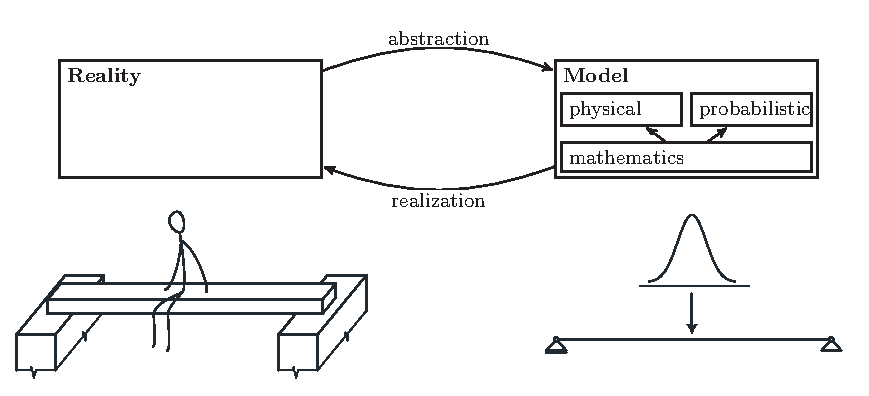
\includegraphics[width=0.8\textwidth]{modeling_overview_all.pdf}
	\caption{Concept of modeling with its main components.}
	\label{fig:mod_overview}
\end{figure}
}   


%******************************************************************************************
%******************************************************************************************
\section{Problem statement} % SPECIFIC
\label{sec:prob_state}

Snow is an important climatic action, which governs the reliability of many structures, particularly of lightweight roofs. These should operate without major structural maintenance for typically 50 years, and their real working life often spans over 100 years. Therefore, it is of utmost importance that the expected actions are adequately anticipated during the design process.

The topic selection is partially motivated by the relatively large number of structural damages and collapses experienced around the world due to snow loads \citep{Geis2011}; e.g. recently in 2005/06 Central Europe, 2010/11 North-Eastern USA. One of the diverse causes of collapses appears to be the inadequate safety level provided by standards \citep{Holicky2009, Meloysund2010}. Further motivations for the study are the perceived inconsistencies in the current European standard regarding exceptional ground snow load, and statistical treatment of snow measurements. The problems seem to be urgent particularly for lowland areas with continental climate where exceptional snowfalls are more likely than in mountains \citep{Sanpaolesi1998}. Thus, the topic has a great importance for Hungary and for neighboring countries. The relevance of the topic is also highlighted by a foreseen revision of design procedures within Eurocode. 

The main issues examined in this study -- with brief description and related questions -- are summarized below (for detailed references see the relevant chapters):

\begin{enumerate}
	\item There is a lack of agreement among reliability experts on the appropriate distribution function for ground snow maxima. Critical examination of current probabilistic snow models and application of statistically established methods are needed. \textit{Which distribution function is the ``best'' to model ground snow extremes? What constitutes an appropriate model?}
	
	\item Statistical uncertainties -- arising from scarcity of observations -- are typically neglected; however, they seem to be important as observation periods are only a small fraction of governing return periods, thus extrapolation to unobserved ranges is inevitable. \textit{How large is the effect of statistical uncertainties on structural reliability? Is their neglect reasonable? How should these uncertainties be taken into account?}
	
	\item Measurements are inevitably contaminated with measurement uncertainty, which is especially important for snow where measuring techniques are often burdened with large uncertainty. \textit{How measurement uncertainty should be taken into account and propagated to structural reliability? Is the current practice, which neglects it, acceptable from reliability point of view? Is its effect on failure probability practically significant?}
	
	\item Current civil engineering provisions are based on the assumption of stationarity; however, recent observations and climate models challenge this. \textit{Is the stationary assumption tenable for snow extremes? What are the practical implications of time-trends for structural reliability?}
	
	%\item Exceptional ground snow load is a ``new action'' in Eurocode that is governing the design of many lightweight structures. Yet, no definition is given in the standard and there is a confusion whether to consider it.  \textit{Is exceptional ground snow load justified from meteorological, statistical, or reliability point of view? What can be a rational definition of it? How large its value should be?}
	
	\item Correlation structure of stochastic processes is almost solely described by Gauss copula; however, this assumption is not corroborated by empirical evidence. \textit{How large is the effect of copula assumption on time-variant structural reliability? Is the current practice conservative for snow loads? How can the copula function uncertainty be treated?}		
\end{enumerate}

%All of these questions are practically motivated and investigated with bearing in mind 

\mynote{
The dominant components, sources of uncertainty are actions, their accurate modeling is important.
Comparative study between Poland and South Africa: Wind climates, the related damage and implications of adopting the Eurocode for wind action on buildings Section 4.1
motivation for wind loads
}


%******************************************************************************************
%******************************************************************************************
\section{Adopted approach}
\label{sec:solu_strat}

To explore the questions listed in Section \ref{sec:prob_state}, methods of structural reliability, mathematical statistics, and conventional civil engineering are applied. The general rationale of the investigations is the same: 
\begin{enumerate}
	\item Identification of potential gaps in current body of knowledge and/or non-conservative assumptions in practice.
	\item Examination of the underlying concepts to support hypothesis formulation, then selection or development of tools for quantitative analysis of the identified questions. 
	\item Qualitative and quantitative comparison of popular civil engineering approaches with more advanced statistical techniques that are able to capture in the former neglected effects.
	\item Parametric analysis using minimal\footnote{Minimal is used in the sense of minimal working example of programming. As simple as possible to capture the essential features of examined issue, but not simpler.} reliability problems that represent generic structures. Consideration of an extended parameter range to cover random variables other than ground snow intensity too.
	\item Illustration of the effects and proposed approaches with real-life examples.
	\item Discussion of the question and results from a broader, decision making perspective.
	\item Formulation of practical recommendations and simplified rules.
\end{enumerate}

\mynote{The latter serve as reference points as they are more sophisticated than those prevalently used in structural reliability and for calibration of standards.}

%******************************************************************************************
%******************************************************************************************
\section{Structure of the thesis}
\label{sec:organization}

The thesis' organization is presented in Figure \ref{fig:thesis_overview}.
After the introduction, an overview of the applied methods and terminology is presented (Chapter \ref{cha:overview}). Then each subsequent chapters (\ref{cha:stat_unc}-\ref{cha:copula}) deal with one or two research questions. These are similarly structured and accompanied with application examples that are intended to highlight the practical importance of the questions and feasibility of proposed approaches. These question-chapters are loosely connected and these connections are indicated by dashed lines in Figure \ref{fig:thesis_overview}. Finally, the study concludes with the summary of the contributions (Chapter \ref{cha:summary}). The appendices gather supplementary materials and technical details in an extent to allow reproducibility. Further supporting materials are available from the following GitHub account: \url{https://github.com/rozsasarpi}.

\begin{figure}[htbp!] 
	\centering
	\begin{tikzpicture}[->,>=stealth',shorten >=1pt,auto,
		thick,main node/.style={circle,draw,
		font=\large\bfseries,minimum size=7mm}]
		
		% Main, chapter nodes
		\node[main node] (1) at (0,0) 		{\ref{cha:intro}};
		\node[main node] (2) at (0,-1.5) 	{\ref{cha:overview}};
		
		\node[main node] (3) at (-3.00,-3)  {\ref{cha:stat_unc}};
		\node[main node] (4) at (-1.00,-3)  {\ref{cha:error}};
		\node[main node] (5) at (1.00,-3) 	{\ref{cha:time_trend}};
		\node[main node] (6) at (3.00,-3) 	{\ref{cha:copula}};
		
		\node[main node] (7) at (0,-4.5) 	{\ref{cha:summary}};
		
		% Encompass contribution chapters, dashed rectangle
		\draw [gray] (-3.75,-2.25) rectangle (3.75,-3.75);
		
		% Structure of contribution chapters
		\node[text width=5cm, anchor=east, right] (S) at (5,-3)
		{\small
		Structure of chapters \ref{cha:stat_unc}-\ref{cha:copula}: \\
		\begin{enumerate}[nolistsep, label=\roman*]
			\item Problem statement
			\item Solution strategy
			\item Results of simple and application examples
			%\item Extension to other random variables
			\item Discussion
			\item Conclusions
		\end{enumerate}
		};

		% Connection between nodes
		\path[every node/.style={font=\small,
				fill=white,inner sep=1pt}]
		% Right-hand-side arrows rendered from top to bottom to
		% achieve proper rendering of labels over arrows.
			
				(5) edge [bend left=50, dotted] node[] {} (S)
				(S) edge [bend left=50, dotted] node[] {} (5)
			
		(1) edge [] node[] {} (2)
		 	 	
		(2) edge [bend left=10] 			node[] {} (3)
			edge [bend left=10] 			node[] {} (4)
			edge [bend left=-10] 			node[] {} (5)
			edge [bend left=-10] 			node[] {} (6)
		
		(3) edge [bend left=10] 			node[] {} (7)
			edge [bend left=-30, dashed] 	node[] {} (5)
			edge [bend left=25, dashed] 	node[] {} (6)
		(4) edge [bend left=10] 			node[] {} (7)
		(5) edge [bend left=-10] 			node[] {} (7)
		(6) edge [bend left=-10] 			node[] {} (7);

		
		% List of chapter names with links
		\node[text width=12cm, anchor=west, right] at (-4.25,-7.25)
		{\small
		\textbf{\ref{cha:intro}} \nameref*{cha:intro} \\
		\textbf{\ref{cha:overview}} \nameref*{cha:overview} \\
		\textbf{\ref{cha:stat_unc}} \nameref*{cha:stat_unc} \\
		\textbf{\ref{cha:error}} \nameref*{cha:error} \\
		\textbf{\ref{cha:time_trend}} \nameref*{cha:time_trend} \\
		\textbf{\ref{cha:copula}} \nameref*{cha:copula} \\
		\textbf{\ref{cha:summary}} \nameref*{cha:summary} \\
		};
				
	\end{tikzpicture}
	\caption{Overview of the organization of the thesis.}
	\label{fig:thesis_overview}
\end{figure}

\mynote{It is important that some of the listed challenges are the same for other extreme actions as well, e.g. wind, thermal actions, traffic, earthquakes. Therefore the chapters contains an \textit{Extension to other random variables} section that puts the findings and conclusions into a broader perspective and indicates the consequences for these other actions as well. It is expected that the research outcomes can be directly used for these as well and can help to draft more consistent standards and to build safer structures.}

%******************************************************************************************
\subsection{Application examples}
% Mirek ~ target beta, system reliability analysis

To emphasize the practical importance and consequences of the examined issues, each one is demonstrated through real-life examples: 
\begin{itemize}
	\item \textit{Turbine hall} of the Hungarian nuclear power plant in Paks. It is an example of probabilistic assessment of safety critical structures. The governing load of the steel hall is snow. Detailed description of the structure is given in Annex \ref{sec:paks}.
	\item \textit{Eiffel-hall} in Budapest. It is a more than 130 years old 95m $\times$ 235m $\approx$ 22000m$^2$ floor area locomotive workshop constructed between 1883 and 1885. The planned change of its function requires the analysis of the structure that serves as an example for probabilistic analysis of existing structures. The governing load of the slender wrought iron hall is snow. Detailed description of the structure is given in Annex \ref{sec:eiffel}.
\end{itemize}

%******************************************************************************************
%******************************************************************************************
\section{Position of the thesis in probabilistic engineering} 

According to \citet{Nowak2000} the origins of probabilistic engineering analysis and construction regulations can be traced back to centuries, even millennia. Although early attempts were not systematic, they recognized the inherent probabilistic nature of engineering design and tried to account for uncertainties in resistances and loads as well. Among the first modern advocates and pioneers of probabilistic design were \citet{Kazinczy1921}, \citet{Mayer1926}, and \citet{Freudenthal1947}, whose outstanding works have shaped the field.
Later other important contributions were made by Ang, Cornell, Der Kiureghian, Ditlevsen,  Elishakoff, Ellingwood, Frangopol, Galambos, Grigoriu, Lind, Melchers, Rackwitz, Turkstra, and Wen.
The results are organized into books, e.g. \citet{Melchers2002,Ditlevsen2007,Nowak2000,Elishakoff2004,Ang2006,Cornell1967,Cristensen1982}.
The field is still  actively researched with overarching scope and applications in almost all engineering fields.

Hungarian researchers also played an important role in the advancement of probabilistic engineering, most notably \citet{Kazinczy1921}. Motivated by scare resources following World War II, Hungary was the first country to adopt semi-probabilistic design philosophy using partial factors for a countrywide code in 1950 \citep{Menyhard1951}. Many Hungarian or Hungary related research engineers contributed and still contribute to the field \citep{Misteth2001, Koris2009, Szalai2011, Logo2011, Rad2011, Honfi2013} along with statisticians and probabilists \citep{Renyi1970, Prekopa1995, Habib2000, Szantai2012, Galambos1978}.
%which are indispensable tools for probabilistic engineering analysis


% Hungary was one of the first country to adopt semi-probabilistic design code. This was motivated by scare resources after the second World War and inspired by Soviet military standards. In the second half of the 20th century Hungarian researchers played and an active role in developing and applying probabilistic concepts in engineering, this era is hallmarked by the towering figure of Endre Mistéth \citep{Misteth2001}. Still by Hungarian researchers with Hungarian origin \cite{Koris2009, Szalai2011, Logo2011, Rad2011} and probability contemporary mathematical theory \cite{Prekopa1995, Habib2000, Szantai2012, Galambos1978}
%
%Building on pioneering work of \citet{Mayer1926} partial safety factor based methods were introduced in the USSR in the form of a technical directive. It regulated the design and construction of reinforced concrete structures during wartime \citep{Farkas2006}.  Motivated by scare resources following World War II, Hungary was the first country to adopt this semi-probabilistic design philosophy using partial factors for a countrywide code in 1950 \citep{Menyhard1951, Gyengo1960}. Others claim the primacy of formulation consistent, partial safety factor based code for Denmark, where this process was started in the 1950s \citep{Ditlevsen2007}.
%
%\citep{Melchers2002,Ditlevsen2007,Nowak2000,Elishakoff2004,Ang2006,Cornell1967,Cristensen1982}


%******************************************************************************************
%******************************************************************************************
\section{Scope and limits} 
\label{sec:scope}

The main questions examined in this study are general and relevant for all basic variables affecting structural reliability, yet the focus is on ground snow extremes. These are analyzed from an engineering point of view, i.e. concentrating on issues with engineering significance, such as structural reliability and design regulations. Less attention is devoted to other questions that might be the interest of statisticians or meteorologists. Solely the time-variant component of ground snow load is analyzed thoroughly, although the time-invariant component: ground to roof conversion factor might be of similar importance. Moreover, the data-driven analyses are restricted to the climatic conditions of the Carpathian Region. The analyses are conducted with other climatic actions in mind, the parametric studies are extended to the range of actions other than snow. Thus the scope of the thesis is extreme ground snow loads but its limits extend to all random variables and stochastic processes considered in probabilistic engineering analysis.

All models in this study are fully statistical, this means that no physical arguments and principles are incorporated. This is a prevalent approach not only in engineering but in other fields as well. To our\footnote{First person plural is used in this study to refer to the candidate's knowledge, work, decision, opinion, etc. The only exception is the formulation of theses in Chapter~\ref{cha:summary}, where first personal singular is used for the same purpose in line with the requirements of the Vásárhelyi Pál Doctoral School.} knowledge, first principle based meteorological models are not yet able to reliably predict extreme snow events. Especially if those are the product of a local atmospheric phenomenon\footnote{In this respect important advances are expected in the future. First principle based extreme event prediction might soon be available by extending the incorporated physical models and increasing the spatial and temporal resolutions of general circulation models. These advances can open up new possibilities to give substantially improved answers to the questions considered here.}. The presented analyses are based on mathematical statistics, e.g. the extreme value theory, which provides a strong theoretical support for the models under consideration.

The two main focuses of probabilistic engineering are (\textit{i}) calculation of probability of rare events such as structural failure (structural reliability); and (\textit{ii}) propagation of uncertainty through physical models. Both are concerned with uncertainty representation and with efficient solution of the posed problems. In this thesis only structural reliability problems are considered.
%within this, both time-variant and time-invariant problems are considered. Furthermore, almost solely only component level analyses are studied, where only a single failure mode contributes to the failure probability. Although structural reliability comprise great many other problems such as systems, random fields, code calibration, etc.

One can categorize uncertainties into the following groups:
\begin{itemize}
	\item physical uncertainty (inherent, irreducible uncertainty in the adopted model space, ``model universe'');
	\item statistical uncertainty (parameter estimation and probabilistic model selection uncertainties);
	\item measurement uncertainty;
	\item model uncertainty (physical model selection uncertainty);
	\item human error.
\end{itemize}

Based on its nature, uncertainty can be aleatory or epistemic. In this framework aleatory uncertainty refers to the uncertainty that cannot be reduced, inherent in the selected model space. While epistemic refers to uncertainty that is reducible, for example by obtaining and incorporating more data. This classification is not absolute and it is always conditioned on the selected model space. 
This thesis deals only with physical, statistical, and measurement uncertainties; and it focuses on epistemic uncertainties.

Since agreement is lacking on the nature, interpretation, and representation of uncertainty, it is not surprising that multitude of concepts are available and applied. These include probability theory, imprecise probability theory, fuzzy set theory, possibility theory, evidence theory, etc. \citep{Corotis2015, Ayyub2006}. In this study we mostly rely on probability theory, but interval analysis, which belongs to imprecise probability theory, is also used to represent a level ignorance that probability distributions cannot. Even within probability theory there is a lack of consensus on interpretation of probability \citep{Hajek2012}. We subscribe to the notion that ``probability does not exist''\footnote{Maybe with the exception of the realm of quantum mechanics, which does not concern us herein.} \citep{Finetti1974} and probability is conditioned on the observer and on the selected model space.

The scrutinized questions cover only a small but important fraction of open questions even in engineering modeling of extreme snow loads and structural reliability. Still not only the treated questions are more general but the provided answers and solutions too. Hence, it is surmised that the findings can also be applied to issues out of the scope of this thesis.

\mynote{The selection is spurred by the projects in which the candidate was involved and by personal interest.}

% Keep in concise and consistent!!
%........................................................................
% ABBREVIATION 
%\nomenclature[z-AASHTO]{AASHTO}{American Association of State Highway and Transportation Officials}
\nomenclature[z-AIC]{AIC}{Akaike information criterion}
\nomenclature[z-AICc]{AICc}{sample size corrected Akaike information criterion}
\nomenclature[z-BIC]{BIC}{Bayesian information criterion}
\nomenclature[z-BMA]{BMA}{Bayesian model averaging}
\nomenclature[z-BP]{BP}{Bayesian posterior}
\nomenclature[z-BPM]{BPM}{Bayesian posterior mean}
\nomenclature[z-BPP]{BPP}{Bayesian posterior predictive}
%\nomenclature[z-cdf]{cdf}{Cumulative probability distribution function}
\nomenclature[z-CI]{CI}{confidence interval}
\nomenclature[z-DI]{DI}{direct integration}
%\nomenclature[z-CEN]{CEN}{European Committee for Standardization} %(Comité Européen de Normalisation)}
%\nomenclature[z-cMC]{cMC}{Crude Monte Carlo}
%\nomenclature[z-EC]{EC}{Eurocode}
\nomenclature[z-eqi]{eqi}{equal tail credible interval}
%\nomenclature[z-FEM]{FEM}{Finite Element Method}
\nomenclature[z-FMA]{FMA}{frequentist model averaging}
\nomenclature[z-FORM]{FORM}{first order reliability method}
\nomenclature[z-GEV]{GEV}{Generalized extreme value distribution}
\nomenclature[z-GMM]{GMM}{Generalized method of moments}
%\nomenclature[z-GoF]{GoF}{Goodness-of-fit measure}
%\nomenclature[z-GUM]{GUM}{Gumbel distribution}
\nomenclature[z-hdi]{hdi}{highest density credible interval}
%\nomenclature[z-isMC]{isMC}{Importance sampling Monte Carlo}
\nomenclature[z-LN2]{LN2}{two-parameter Lognormal distribution}
\nomenclature[z-LN3]{LN3}{three-parameter Lognormal distribution}
\nomenclature[z-LR]{LR}{likelihood ratio}
\nomenclature[z-MA]{MA}{model averaging}
\nomenclature[z-mad]{mad}{median absolute deviation}
\nomenclature[z-MCMC]{MCMC}{Markov chain Monte Carlo}
\nomenclature[z-MC]{MC}{Monte Carlo}
\nomenclature[z-ML]{ML}{maximum likelihood}
\nomenclature[z-MM]{MM}{method of moments}
\nomenclature[z-MU]{MM}{measurement uncertainty}
%\nomenclature[z-ME]{ME}{Maximum entropy}

\nomenclature[z-N]{N}{Normal distribution}
%\nomenclature[z-pdf]{pdf}{Probability density function}
\nomenclature[z-rot]{rot}{rotated}
\nomenclature[z-SORM]{SORM}{second order reliability method}
\nomenclature[z-std]{std}{standard deviation}
\nomenclature[z-SWE]{SWE}{snow water equivalent}
\nomenclature[z-ZAMG]{ZAMG}{Central Institution for Meteorology and Geodynamics}



%........................................................................
% ROMAN
%\nomenclature[a-Bf]{$B$}{Bayes factor}
\nomenclature[a-AIC]{$AIC$}{Akaike information criterion}
\nomenclature[a-AICc]{$AICc$}{sample size corrected Akaike information criterion}
\nomenclature[a-BIC]{$BIC$}{Bayesian information criterion}
\nomenclature[a-b]{$b$}{Bayesian weight}
\nomenclature[a-CV]{$CV$}{coefficient of variation}
\nomenclature[a-C]{$C(.)$}{copula function}
\nomenclature[a-Ffun]{$F(.)$}{cumulative probability distribution function}
\nomenclature[a-ffun]{$f(.)$}{probability density function}
\nomenclature[a-gfun]{$g(.)$}{performance function}
\nomenclature[a-L]{$L(.)/L$}{likelihood function/value}
\nomenclature[a-L]{$L_\mathrm{p}(.)$}{pairwise likelihood function}
\nomenclature[a-M]{$M$}{model}
\nomenclature[a-n]{$n$}{number of observations}
\nomenclature[a-P]{$P$}{probability of an event}
\nomenclature[a-pp]{$p(.)$}{probability density/mass function}
\nomenclature[a-Pf]{$P_\mathrm{f}$}{probability of failure}
\nomenclature[a-RP]{$RP$}{return period}
\nomenclature[a-RV]{$RV$}{return value}
\nomenclature[a-t]{$t$}{time or any strictly monotonically increasing parameter}
\nomenclature[a-tt]{$t(.)/t_2(.)$}{univariate/bivariate Student (or \textit{t})  cumulative distribution function}
\nomenclature[a-XX]{$X/\bf{X}$}{random variable(s)}
\nomenclature[a-XX]{$x/\bf{x}$}{realization(s) of a random variable or independent variable}
\nomenclature[a-w]{$w$}{Akaike weight}

%........................................................................
% GREEK
\nomenclature[g-alpha]{$\alpha$}{FORM sensitivity factor}
\nomenclature[g-beta]{$\beta$}{reliability index}
%\nomenclature[g-lambda]{$\lambda$}{Lagrange multiplier}
\nomenclature[g-chi]{$\chi$}{load ratio}
\nomenclature[g-epsr]{$\epsilon_\mathrm{r}$}{interval radius for measurement uncertainty}
\nomenclature[g-nu]{$\nu^+$}{out-crossing rate}
\nomenclature[g-Phi]{$\Phi(.)/\Phi_2(.)$}{univariate/bivariate standard Normal cumulative probability distribution function}
\nomenclature[g-rho]{$\rho$}{Pearson's rho (correlation coefficient)}
\nomenclature[g-tau]{$\tau$}{Kendall's tau (correlation coefficient)/dummy variable}
\nomenclature[g-tauF]{$\tau_\mathrm{F}$}{correlation length}
\nomenclature[g-theta]{$\theta/\boldsymbol{\theta }$}{inferred parameter(s)}
\nomenclature[g-xi]{$\xi$}{shape parameter of GEV}

%........................................................................
% OTHER (mainly operator)
\nomenclature[x-Exp]{E(.)}{mean value, expectation operator}
\nomenclature[x-Var]{Var(.)}{variance operator}
\nomenclature[x-conv]{$*$}{convolution operator}
%\nomenclature[x-grad]{$\nabla(.)$}{Gradient operator}
\nomenclature[x-distr]{$\sim$}{distributed as}
\nomenclature[x-distr]{$\dot{\sim}$}{asymptotically distributed as}
\nomenclature[x-interval]{$\underline{\mathrm{par}}, \overline{\mathrm{par}}$}{lower and upper interval bounds of a parameter (par)}

%........................................................................
% SUBSCRIPT
\nomenclature[s-i]{$i, j$}{loop counter}
%\nomenclature[s-j]{$j$}{Loop counter}

% WITH ECONOMIC OPTIMISATION
%	\begin{tikzpicture}[->,>=stealth',shorten >=1pt,auto,
%		thick,main node/.style={circle,draw,
%		font=\large\bfseries,minimum size=7mm}]
%		
%		% Main, chapter nodes
%		\node[main node] (1) at (0,0) {\ref{cha:intro}};
%		\node[main node] (2) at (0,-1.5) {\ref{cha:overview}};
%		
%		\node[main node] (5) at (-0.75,-3) {\ref{cha:time_trend}};
%		\node[main node] (4) at (-2.25,-3) {\ref{cha:error}};
%		\node[main node] (3) at (-3.75,-3) {\ref{cha:stat_unc}};
%		\node[main node] (6) at (0.75,-3) {\ref{cha:exceptional}};
%		\node[main node] (7) at (2.25,-3) {\ref{cha:eco_cost_opti}};
%		\node[main node] (8) at (3.75,-3) {\ref{cha:copula}};
%		
%		\node[main node] (9) at (0,-4.5) {\ref{cha:summary}};
%		
%		% Encompass contribution chapters, dashed rectangle
%		\draw [dashed] (-4.25,-2.25) rectangle (4.25,-3.75);
%		
%		% Structure of contribution chapters
%		\node[text width=5cm, anchor=east, right] (S) at (5,-3)
%		{\small
%		Structure of chapters \ref{cha:stat_unc}-\ref{cha:copula}: \\
%		\begin{enumerate}[nolistsep, label=\roman*]
%			\item Problem statement
%			\item Solution strategy
%			\item Results and discussion
%			%\item Extension to other random variables
%			\item Application example
%			\item Conclusions
%		\end{enumerate}
%		};
%
%		% Connection between nodes
%		\path[every node/.style={font=\small,
%				fill=white,inner sep=1pt}]
%		% Right-hand-side arrows rendered from top to bottom to
%		% achieve proper rendering of labels over arrows.
%			
%				(7) edge [bend left=50, dashed] node[] {} (S)
%				(S) edge [bend left=50, dashed] node[] {} (7)
%			
%		(1) edge [] node[] {} (2)
%		 	 	
%		(2) edge [bend left=0] node[] {} (3)
%			edge [bend left=10] node[] {} (4)
%			edge [bend left=10] node[] {} (5)
%			edge [bend left=-10] node[] {} (6)
%			edge [bend left=-10] node[] {} (7)
%			edge [bend left=0] node[] {} (8)
%		
%		(3) edge [bend left=0] node[] {} (9)
%			edge [bend left=-30, dashed] node[] {} (5)
%			edge [bend left=30, dashed] node[] {} (6)
%			edge [bend left=30, dashed] node[] {} (7)
%		(4) edge [bend left=10] node[] {} (9)
%		(5) edge [bend left=10] node[] {} (9)
%		(6) edge [bend left=-10] node[] {} (9)
%		(7) edge [bend left=-10] node[] {} (9)
%		(8) edge [bend left=0] node[] {} (9);
%		
%		% List of chapter names with links
%		\node[text width=10cm, anchor=west, right] at (-4.25,-7.25)
%		{\small
%		\textbf{\ref{cha:intro}} \nameref*{cha:intro} \\
%		\textbf{\ref{cha:overview}} \nameref*{cha:overview} \\
%		\textbf{\ref{cha:stat_unc}} \nameref*{cha:stat_unc} \\
%		\textbf{\ref{cha:error}} \nameref*{cha:error} \\
%		\textbf{\ref{cha:time_trend}} \nameref*{cha:time_trend} \\
%		\textbf{\ref{cha:exceptional}} \nameref*{cha:exceptional} \\
%		\textbf{\ref{cha:eco_cost_opti}} \nameref*{cha:eco_cost_opti} \\
%		\textbf{\ref{cha:copula}} \nameref*{cha:copula} \\
%		\textbf{\ref{cha:summary}} \nameref*{cha:summary} \\
%		};
%				
%	\end{tikzpicture}
%*******************************************************************************
%****************************** Second Chapter *********************************
%*******************************************************************************

\chapter{Overview of uncertainty modeling and propagation}
\label{cha:overview}

% **************************** Define Graphics Path **************************
\ifpdf
    \graphicspath{{Chapter2/Figs/Raster/}{Chapter2/Figs/PDF/}{Chapter2/Figs/}}
\else
    \graphicspath{{Chapter2/Figs/Vector/}{Chapter2/Figs/}}
\fi

% **************************** Chapter Abstract ******************************
\leftskip=1cm
\noindent
\emph{This chapter presents a brief overview of uncertainty modeling and structural reliability. It focuses on topics discussed in this dissertation from an engineering point of view. The main aim is to present the concepts, terms, notations, and methods used in further chapters. Emphasis is put on subjects that are typically insufficiently treated, overly simplified, or neglected in current civil engineering practice.}

\leftskip=0pt\rightskip=0pt


%****************************************************************************************
%****************************************************************************************
\section{Uncertainty modeling}

Statistical and interval based approaches are used to model and to propagate uncertainties. The former is used for most of the calculations, while interval analysis is only applied to represent measurement uncertainty and to compare with statistical approaches. Thus, interval analysis is introduced in the relevant chapter (Chapter~\ref{cha:error}). Since the mathematical machinery often appreciably differs from chapter to chapter, the particular, chapter-specific methods are introduced there. Here only the common, in multiple chapters utilized concepts are exposed.

The statistical analyses are completed using two main paradigms: frequentist and Bayesian statistics. The former views probability as a long-run frequency and bases inference on comparing the relative likelihood of datasets given a parameter value. Probability in the latter reflects the analyst's current state of knowledge using all available  information 
(``degree  of  belief''\footnote{It is often termed subjective probability; however, subjective here is not used in its everyday meaning. Instead it reflects the analyst's inevitable modeling assumptions and decisions, which are not solely based on the information conveyed by the data but on his or her expert judgment. Still the rationality and consistency are maintained: two analysts with the same experience and information would came up with the same inference.})
and  bases inference  on the relative evidence of the parameter values given a dataset \citep{Spiegelhalter2009, Cornell1970}. The latter is also regarded as the extension of classical logic \citep{Jaynes2003}.
It is out of the scope of this study to compare the frequentist and Bayesian paradigms in detail and to expose  the  deep  philosophical differences, see \citet{Jaynes2003, Barnett1999}. A brief comparison is presented in Table \ref{tab:freq_bay}, from which the most relevant for us are detailed in later sections. For a more comprehensive, practically oriented comparison see \citet{Wagenmakers2008, Jaynes1976}.
In later chapters mostly the Bayesian statistics is advocated and used due to that (\textit{i}) it represents all parameters with probability distribution thus enables the propagation and integration their uncertainty in further analysis, e.g. decision making; (\textit{ii}) allows to combine information from different sources; (\textit{iii}) and can efficiently handle complex problems with messy data.

The statistical techniques applied to estimate parameters, to construct uncertainty intervals, to account for distribution type uncertainty, to evaluate goodness-of-it, and to predict future observations are detailed in Annex~\ref{sec:stat_tools}. The descriptions are given in an extent to enable reproducibility.
The statistical techniques and notation used in further chapters are summarized in Table~\ref{tab:stat_methods_notations}.

% make the cells better looking!
\begin{table}
\caption{A brief comparison of frequentist and Bayesian statistics.}
\centering
\label{tab:freq_bay}
\small
\bgroup
\def\arraystretch{1.2}
    \begin{tabular}{m{0.24\textwidth} | m{0.35\textwidth} | m{0.35\textwidth}}
    \toprule
    Category & Frequentist  & Bayesian \\ 
    \midrule
    \rowcolor{lightgrey} Probability, $P$: & long-run frequency  &  degree of belief \\
    Parameters: & fixed but unknown &  random variables \\
    \rowcolor{lightgrey} Focuses on: & variability of data  &   uncertainty of knowledge \\
    Mathematical \newline machinery: & sampling distribution, repeated hypothetical experiments & Bayes' theorem, fixed data\\
    \rowcolor{lightgrey} Answers/calculates: & $P\left(\mathrm{data}|\mathrm{hypothesis}\right)$ &  $P\left(\mathrm{hypothesis}|\mathrm{data}\right)$ \\
    Source of information: & data (observations) &   data (observations) + prior belief \\
    \bottomrule
    \end{tabular}
\egroup
\end{table}



\mynote{not counting for cognitive differences and limitations (this latter problem is solved by Jaynes' robot)}
\mynote{note should be added that the term frequentist and bayesian a little vague, they should be understood with the given description and organization}



%\begin{landscape}
\begin{sidewaystable}[ht]
\caption{Summary of applied statistical methods and notations, for details see Annex~\ref{sec:stat_tools}.}
\centering
\label{tab:stat_methods_notations}
\small
	\begin{threeparttable}
    \begin{tabular}{lllll}
    \toprule
    Name\tnote{*} & Point estimate & \multicolumn{2}{l}{Uncertainty interval} & Model averaging \\
    \midrule
    Method of moments & MM  & -- & & -- \\
    \rowcolor{lightgrey}
    Generalized method of moments\tnote{\textdagger} & GMM  & delta & delta method\tnote{$\ddagger$} & -- \\ 
    \midrule
    \rowcolor{lightgrey}
    Maximum likelihood\tnote{\textdagger}  & ML  & delta & delta method & FMA (Eq.\ref{eq:FMA_point}-\ref{eq:FMA_var}) \\
    \rowcolor{lightgrey}
    ~ & ~  & proflike & profile likelihood  & ~ \\
    \rowcolor{lightgrey}
    ~ & ~  & bootstrap & bootstrapping  & ~  \\ 
    \midrule
    Bayesian posterior mean & BPM & hdi & highest density interval & BMA (Eq.\ref{eq:BMA}) \\
    ~ & ~ & eqi & equal tail interval & ~ \\
    Bayesian posterior predictive & BPP, (Eq.\ref{eq:postpred})& -- & & -- \\ 
    \bottomrule
    \end{tabular}
    \begin{tablenotes}
    \item[*] Examples for notation: \\
    ML-delta: maximum likelihood estimate with uncertainty interval constructed using delta method; \\
    BMA-BPM-hdi: Bayesian model averaged posterior mean estimate with highest density uncertainty interval.
    \item[\textdagger] \colorbox{lightgrey}{Frequentist paradigm.}
    \item[$\ddagger$] Similar to classic delta method but based on a special weighting matrix, see Section \ref{sec:interval_estimates}. 
    \item -- Not applicable/not available.
    \end{tablenotes}
    \end{threeparttable}
\end{sidewaystable}
%\end{landscape}

\mynote{summary, overview figure about treating parameter estimation and model selection uncertainty, might be better in Chapter 3}

%******************************************************************************************
%******************************************************************************************
\section{Structural reliability}
Structural reliability is concerned with the probabilistic analysis of engineering structures; most often this means the calculation of the failure probability of a structure with uncertain properties and subjected to uncertain actions. This problem is formulated using the limit state concept, which states that the boundary between safe and failure domain is sharp: characterized by a sudden change in performance. Accordingly, the related function is termed as performance function, $g(\mathbf{X})$. The limit state, $g(\mathbf{X})=0$, separates the disjoint safe and failure regions (Fig. \ref{fig:joint_dens}). The failure probability can be calculated as the integral of the joint density function of the random variables over the failure domain\footnote{This simple formulation is given for clarity, a more general formulation would include time, more general probabilistic models, and systems as well.}:
\begin{equation}
	\label{eq:Pf_general}
	 %{P_{\mathrm{f}}} = P\left( {g\left( {\bf{X}} \right) < 0} \right) = \int\limits_{g\left( {\bf{X}} \right) < 0} {{f_{\bf{X}}}({\bf{x}}) \cdot \mathrm{d}{\bf{x}}}.
	 {P_{\mathrm{f}}} = P\left( {g\left( {\bf{X}} \right) < 0} \right) = \int\limits_{g\left( {\bf{X}} \right) < 0} {p({\bf{x}}) \cdot \mathrm{d}{\bf{x}}}
\end{equation}
where $p(.)$ represents a probability density function that is identified by its argument. For example $p(x)$ and $p(y)$ are in general completely different functions. This notation allows greater clarity and conciseness than in reliability engineering typically used notation, $p(x) \equiv f_X(x)$.

The two main challenges in structural reliability are the inference of probabilistic models in the face of information scarcity, and the calculation of the typically high-dimensional integral (Eq.\ref{eq:Pf_general}). The integral is usually approximated by numerical techniques tailored for the particular features of structural reliability problems. These aim to reduce the required number of performance state function evaluations to minimal.

In this thesis, unless otherwise stated, the first order reliability method (FORM) \citep{Hasofer1974} is used for approximating the integral. It is sufficiently accurate for most structural engineering problems \citep{EN0}, though the presented calculations are often verified by more accurate methods, such as second order reliability method (SORM), Monte Carlo simulation (MC), and importance sampling Monte Carlo simulation (isMC).

The improved Hasofer-Lind-Rackwitz-Fiessler algorithm \citep{Rackwitz1979, Zhang1995} is used to solve the constrained optimization problem in FORM. For correlated random variables -- unless otherwise stated -- the Nataf transformation \citep{Liu1986} with Cholesky decomposition is used to obtain independent, normally distributed random variables. The asymptotic formula of \citet{Breitung1984} is used as a correction term in SORM. For isMC multivariate normal distribution used.

\begin{figure}[htbp!] 
	\centering    
	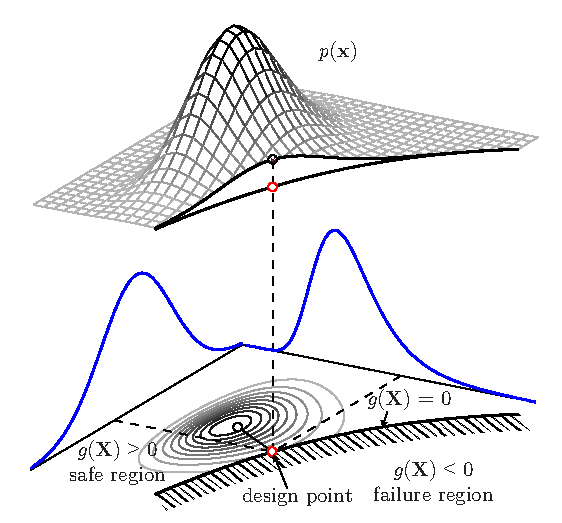
\includegraphics[width=0.6\textwidth]{joint_dens_illustration_fine_db.pdf}
	\caption{Illustration of limit state function, failure and safe regions, and design point.}
	\label{fig:joint_dens}
\end{figure}
\chapter{Effect of statistical uncertainties}
\label{cha:stat_unc}

% **************************** Define Graphics Path **************************
\ifpdf
    \graphicspath{{Chapter3/Figs/Raster/}{Chapter3/Figs/PDF/}{Chapter3/Figs/}}
\else
    \graphicspath{{Chapter3/Figs/Vector/}{Chapter3/Figs/}}
\fi

% **************************** Chapter Abstract ******************************
\leftskip=1cm
\noindent
\emph{This chapter studies the effect of commonly neglected statistical uncertainties on representative fractiles and on structural reliability. The failure probability of a generic structural member, subjected to snow load is analyzed using frequentist and Bayesian techniques to quantify parameter estimation and model selection uncertainties in ground snow load. Various variable to dead load ratios are considered to cover a wide range of real structures. The analysis reveals that statistical uncertainties may have a substantial effect on  reliability. By accounting for  parameter estimation uncertainty,  the failure probability can increase by  more than  an  order  of  magnitude. Bayesian posterior predictive distribution is recommended to incorporate parameter estimation uncertainty in reliability studies.}

\leftskip=0pt\rightskip=0pt

%****************************************************************************************
%****************************************************************************************
\section{Problem statement and the state of the art}

One of the main concerns in structural reliability is the calculation of very small probabilities, such as events expected to occur once in 10000 years. A major difficulty in this is that actions, which structures should withstand, are inferred from 50-100 years of observations. This information might be supplemented by phenomenological or theoretical models but these are seldom available or far too complex to be used in engineering design. 

Hence, probabilistic models of actions are affected by substantial uncertainty, which might dominate the reliability \citep{Coles2003catastrophes}. These uncertainties, which are related to the identification of the probabilistic model on the basis of limited data, are referred hereinafter as statistical uncertainties. Only modeling of a random variable is considered, hence the statistical model uncertainty means the uncertainty in the selection of probabilistic model (distribution function), and the statistical parameter estimation uncertainty refers to the uncertainty in the identification of unknown parameters (e.g. location, scale, shape) of a particular distribution. These two are not entirely separable but it is convenient to use both terms. Statistical uncertainties stem from the scarcity of available information and inevitably present for every probabilistic models. For simplicity they are referred to as parameter estimation and model selection uncertainties.

In reliability studies and standardization statistical uncertainties are routinely neglected \citep{Sanpaolesi1998, Coles2003fully_prob, Sisson2006}. However, this violates a basic requirement of probability calculation, namely that all information should be incorporated and all uncertainties accounted for \citep{Kiureghian1989}. The aim of this section is to explore the effect of this omission on selected fractiles and on structural reliability. Moreover, it critically compares some statistical approaches to incorporate statistical uncertainties into probabilistic models.

%Although the practical calculations are performed on snow extremes, it is expected that the findings can be beneficial for other extremes as well, e.g. there is an ongoing revision of wind loads in Eurocode (WG7) with many overlapping challenges with those of snow loads.

%Hence, the probabilistic models are subjected to substantial statistical uncertainties, i.e. uncertainty in model selection and uncertainty in parameter estimation The current civil engineering practice typically neglects these uncertainties or inadequately addresses them.

%****************************************************************************************
%****************************************************************************************
\section{Solution strategy}
The meteorological actions on structures are almost solely described by statistical distributions since the underlying natural phenomena are too complex to be represented by physical models. This approach is adopted here and the ground snow load intensity is modeled by a single random variable.
  
In line with the current engineering practice the block method \citep{Coles2001} is applied. The block length is one year, covering a whole winter season. The annual ground snow maxima are treated as a sample for each location. The potentially more effective multiple block maxima or smaller block lengths are discarded, since the accumulative nature of snow loads makes it difficult to identify peaks and to justify their independence. For the same reason the peak over threshold approach \citep{Reiss2007} was also not used. To account for dependence between maxima from the same winter season a stochastic process based approach is presented in Chapter~\ref{cha:copula}.

For other actions the dependence of maxima is typically lower, thus multiple block maxima and peak-over threshold approaches are advised to be considered. These methods often extends the sample size by orders of magnitude, thus might substantially reduce statistical uncertainties. For wind speed maxima it is demonstrated that these approaches can lead to 70\% reduction in confidence interval for 1000-year fractiles compared with the annual block maxima approach \citep{RozsasREC2016wind}.

Since the main goal of this chapter is to demonstrate the effect of neglecting statistical uncertainties we believe that it is sufficient to use the one year block approach. This creates common ground for comparison, though in future works approaches that use more information should be considered.

Observations from the Carpathian Region are used to infer the distribution parameters (Section~\ref{sec:data_under_study}). The statistical and structural reliability machinery presented in Section \ref{cha:overview} is utilized to explore the effect of statistical uncertainties on representative fractiles and on structural reliability, and to identify the appropriate distribution type for ground snow maxima.

%\mynote{praise the approach compared to studies where the representative values interpolated}
%The widespread approach is to use the measurements of meteorological stations, infer representative values, and spatially interpolate them to obtain maps. In contrast, here the gap filling is done through interpolation and using meteorological models in space and time too on the level of daily snow water equivalent observations. With the exception of analyzing the maxima these analyses are done by meteorologists and provided in a database (ref).
%Turkey - ASCE \citep{Durmaz2006}

%****************************************************************************************
%****************************************************************************************
\subsection{Data under study}
\label{sec:data_under_study}
The meteorological data are obtained from the CarpatClim database, which is the outcome of a cooperation between nine countries of the Carpathian Region \citep{Szalai2013}. The research is completed under the leadership of the Hungarian Meteorological Service that coordinated the joint effort of the meteorological institutions of Austria, Croatia, Czech Republic, Poland, Romania, Serbia, Slovakia and Ukraine.

The database provides snow water equivalents (SWE) in about 10~km  spatial and daily temporal resolution that corresponds to the period from 1961 to 2010. The daily maxima are recorded in the database. The climatological grid covers the region between latitudes 44°N and 50°N, and longitudes 17°E and 27°E (Figure~\ref{fig:carp_stations}-\ref{fig:elevation_map}). The data are gathered from 288 climate stations and 355 precipitation stations with relatively homogeneous spatial distribution. These are homogenized and spatially interpolated using meteorological and  statistical models, missing data are also filled in using these models. The post-processed data are available in the database. 


\mynote{on the slides of Mónika Lakatos 415 climate stations and 904 precipitation stations are mentioned, this is in conflict with the official website of the project;
missing data is filled by model predictions, should be added}

\begin{figure}[htbp!]
	\centering    
	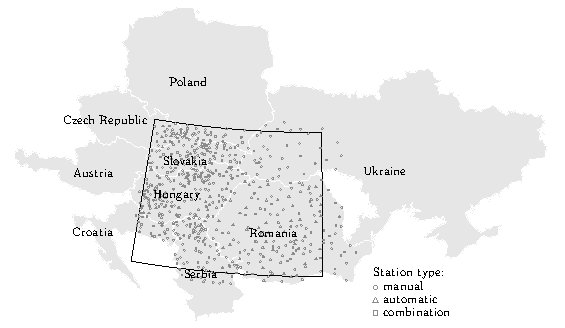
\includegraphics[width=1\textwidth]{carp_map_stations_ai.pdf}
	\caption{Illustration of the studied region (black frame) with involved countries and meteorological stations.}
	\label{fig:carp_stations}
\end{figure}

\begin{figure}[htbp!]
	\begin{subfigure}[b]{0.49\textwidth}    
		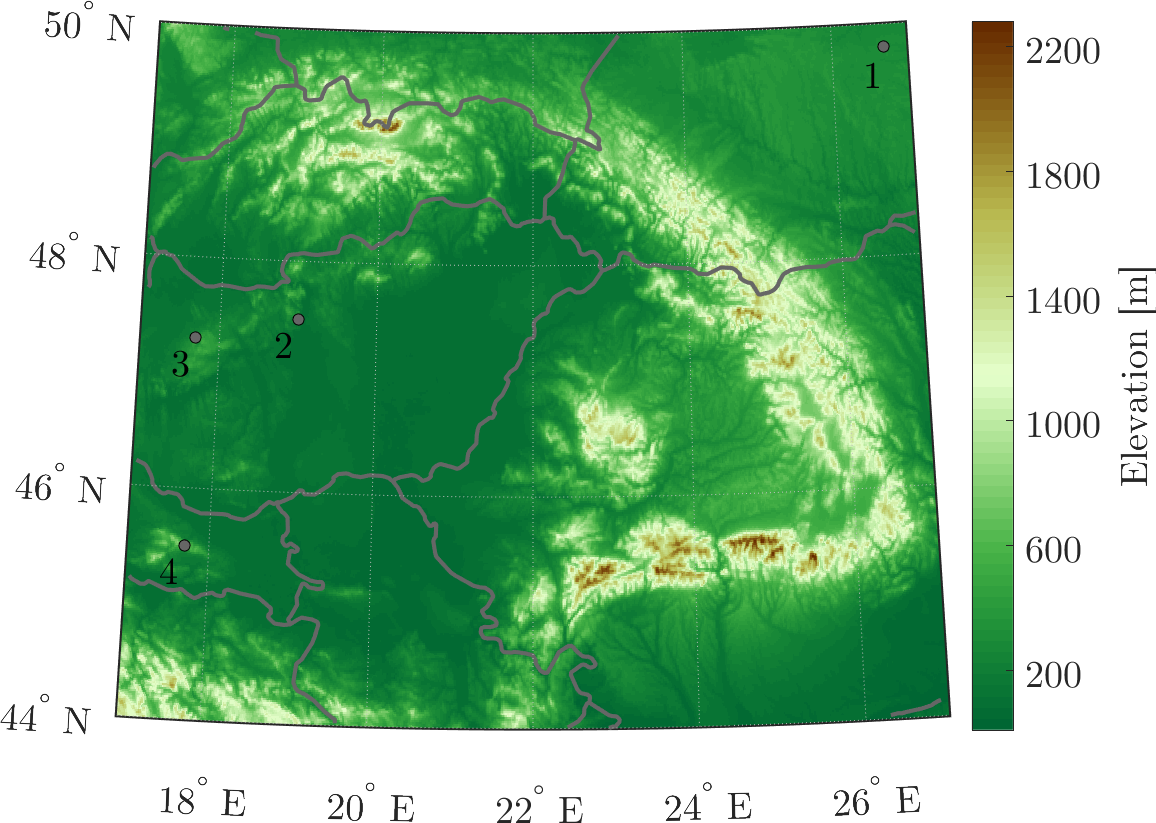
\includegraphics[width=\textwidth]{elevation_map_carpathian_region.png}
		\caption{Elevation map.}
		\label{fig:elevation_map}
	\end{subfigure}
	\hfill
	\begin{subfigure}[b]{0.49\textwidth}
		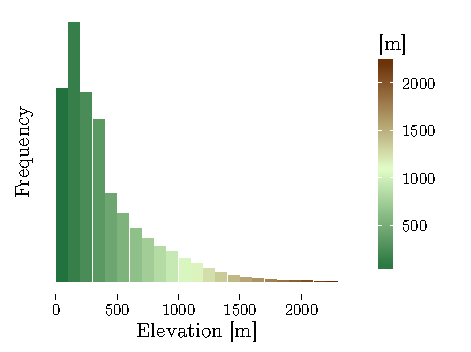
\includegraphics[width=\textwidth]{hist_elevation.pdf}
		\caption{Elevation histogram.}
		\label{fig:elevation_hist}
	\end{subfigure}
	\caption{Illustration of the studied Carpathian region with elevation data with selected locations' ID (Table~\ref{tab:loc_parmest}).}
\end{figure}

Information about the available snow water equivalent data is taken verbatim from the supplementary document of the CarpatClim project \citep{Szalai2013}:
\begin{itemize}
	\item[] ``The water equivalent of a snow cover is the vertical depth of the water that would be obtained by melting the snow cover \citep{WMO2008}.''
	\item[] ``a snow cover model employed operationally at ZAMG [Central Institution for Meteorology and Geodynamics, Austria], was applied to generate a 0.1° latitude/longitude grid of daily mean snow cover and corresponding estimated water equivalent and snow depth simulations. The applied model is based on pre-finished CARPATCLIM grids of mean air temperature [°C], precipitation sum [mm] and relative air humidity [\%]. They are processed by the snow cover model regarding three main parts \textit{accumulation of snow cover, ablation of snow cover and transformation of SWE to snow depth} [emphasis in the original].''
\end{itemize}
Further details about the applied procedures can be found in the cited document.

Uncertainty due to measurement error and due to the approximate nature of meteorological models are neglected. Unless otherwise noted this approach is taken in all chapters, Chapter~\ref{cha:error} deals with this issue in details.


\mynote{images should be improved, country names should be added + precipitation and climate stations}

%****************************************************************************************
%****************************************************************************************
%\section{Distribution of annual ground snow maxima}
%
%In respect of the distribution of ground snow maxima no international consensus has been reached so far. Some commonly used distribution types with regions:
%\begin{itemize}
% \item In Europe Gumbel distribution is typical, it is used for constructing characteristic ground snow maps for most CEN countries \citep{Sanpaolesi1998}.
% \item The Czech Republic derived its snow map using three-parameter Lognormal distribution \citep{Krivy2010}.
% \item In the United States two-parameter Lognormal distribution is adopted in \cite{ASCE2010} based on the research of \citet{Ellingwood1984}.
% \item In Colorado state Normal, Gumbel, three-parameter Lognormal, three-parameter Fréchet, three-parameter Gamma, and three-parameter Loggamma distributions are used and various statistical goodness-of-fit measures are used to select the most appropriate for each site \citep{SEAC2007}.
%\end{itemize}
%Countries even with similar climatic conditions often use different types that typically yield to similar characteristic values but their tail -- governing the failure probability -- is substantially different.
%
%%****************************************************************************************
%\subsubsection*{Generalized extreme value distribution, GEV}
%
%The mathematical support is given by the extreme value theory that states that independent, identically distributed block maxima will asymptotically converge to the generalized extreme value family, irrespectively of the parent distribution \citep{Coles2001, Reiss2007}.
%The standard parametrization of GEV distribution is used with shape ($\xi$), scale ($\sigma$) and location ($\mu$) parameters, see Appendix~\ref{ap:prob_models}, Eq.~\ref{eq:gev_cdf}. The GEV distribution family comprises three special types: Weibull ($\xi < 0$), Gumbel ($\xi = 0$) and Fréchet ($\xi > 0$), see Figure~\ref{fig:gev_skewness}. The first has an asymptotic upper bound while the latter two are unbounded.
%
%
%\subsubsection*{Lognormal distribution}
%
%It is a heavy tailed distribution with $[0,\infty]$ domain that fits better to the majority of the natural phenomena than the typical domain of GEV. Nevertheless, it is not supported by theoretical considerations and unbounded over its whole parameter domain.
%
%The three-parameter Lognormal is the generalization of two-parameter Lognormal by adding a third parameter that shifts the distribution on horizontal axis \citep{Singh1998}.


%****************************************************************************************
\section{Effect on representative fractiles}
Parameter estimation and model selection uncertainty quantifications are conducted for multiple locations of the Carpathian Region. The results of three representative locations are presented in more details: Location 1, 2 and 3 are identified as likely belonging to Weibull, Fréchet and Gumbel families, respectively (Table~\ref{tab:loc_parmest}). To examine the annual ground snow load of other locations an online, interactive snow map is developed by the candidate (Annex~\ref{sec:int_snow_map}). Among others, it can be used to explore the effect of statistical uncertainties and to obtain characteristic ground snow loads.

\begin{table}[htbp!]
\caption{Characteristics of selected locations to illustrate the effect of statistical uncertainties on representative fractiles.}
\centering
\label{tab:loc_parmest}
\small
	\begin{threeparttable}
    \begin{tabular}{l l l l l}
    \toprule
    Location ID\tnote{*}  & Description & Representative of & Elevation [m] & Coordinates  \\
    \midrule
    \rowcolor{lightgrey} 1 (300)  & Ukraine, highland & Weibull & 299 & 49.8°N 26.7°E   \\
    2 (2735)  & Hungary, lowland & Fréchet & 241 & 47.3°N 17.7°E   \\
    \rowcolor{lightgrey} 3 (4553)  & Croatia, highland & Gumbel & 753 & 45.5°N 17.7°E   \\
    4 (2546)  & Hungary, lowland & Fréchet\tnote{\textdagger} & 226 & 47.5°N 19.0°E   \\
    \bottomrule
    \end{tabular}
    \begin{tablenotes}
        \item[*] The first number is used as an identifier here, while the second -- in brackets -- is related to the database.
        \item[\textdagger] Ambiguous, close to Gumbel.
    \end{tablenotes}
    \end{threeparttable}
\end{table}


Two-parameter Lognormal (LN2), three-parameter Lognormal (LN3), Gumbel and Generalized extreme value (GEV) distributions are selected for the comparative analysis (see Annex \ref{sec:distr_fun}). The LN2 model is typically adopted in the USA \citep{ASCE2010} based on the research of \citet{Ellingwood1984}, while the Czech Republic derived its snow map using LN3 distribution \citep{Krivy2010}. The Gumbel model is wide-spread in Europe \citep{Sanpaolesi1998, JCSS_load}. The GEV distribution comprises the Gumbel as a special type and it is supported by the extreme value theory \citep{Coles2001}. The standard parametrization of GEV distribution is used with shape ($\xi$), scale ($\sigma$) and location ($\mu$) parameters, see Appendix~\ref{sec:distr_fun}, Eq.~\ref{eq:gev_cdf}. The GEV distribution family comprises three special types: Weibull ($\xi < 0$), Gumbel ($\xi = 0$) and Fréchet ($\xi > 0$), see Figure~\ref{fig:gev_skewness}. The first has an asymptotic upper bound while the latter two are unbounded.

\begin{figure}[htbp!]
	\centering    
	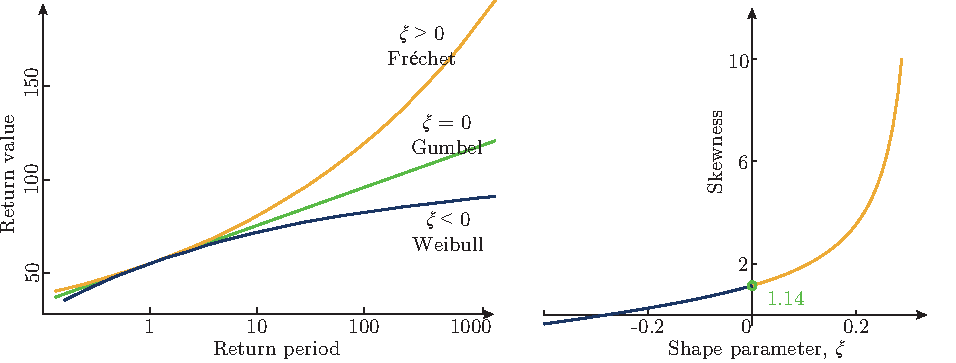
\includegraphics[width=1\textwidth]{GEV_return_value_plot_and_skewness.pdf}
	\caption{Illustration of GEV distribution family in Gumbel space (left), and the related skewness (right).}
	\label{fig:gev_skewness}
\end{figure}

Generalized method of moments (GMM), maximum likelihood (ML), and Bayesian (B) approaches are applied to infer the parameters of the selected distributions. Uncertainty intervals are constructed using delta method, profile likelihood, and bootstrapping in the frequentist paradigm, and highest density and equal tail posterior distribution intervals in the Bayesian one\footnote{These methods and terms are introduced in Chapter~\ref{cha:overview} and in Annex~\ref{sec:stat_tools}.}. An important advantage of the Bayesian approach is that it treats unknown parameters as random variables, hence the incorporation of parameter estimation uncertainty into the model is straightforward. This is done by using the posterior predictive distribution (Eq.\ref{eq:postpred}).

%.......................................................................................
\subsection{Return value--return period plots}

Maximum likelihood method is used to infer the distribution parameters and the results are plotted in Gumbel space (Annex~\ref{sec:prob_plots}). Figure~\ref{fig:loc1_2x2} compares the distribution functions fitted to the observations for Location 1. The edges of the colored ranges are the 90\% confidence intervals obtained by delta method\footnote{The coloring is ``ink-preserving'': the same ``amount of ink'' is used for every vertical section, hence creating a linear transition from the narrowest (dark blue) to the widest interval (white). In a particular 2$\times$2 figure, equal ranges have the same color on each subplot, thus the models are directly comparable based on coloring as well.}. From the plots it is clear that the model type substantially influences the extent of the uncertainty interval. The GEV plot shows that the observations likely belong to the Weibull family and have an upper bound. The other three distributions cannot capture such feature, since they have no upper bound by definition. The difference among the models becomes significant with increasing return period. Similar return value--return period plots are presented in Figure~\ref{fig:loc2_2x2} and \ref{fig:loc3_2x2} for Locations 2 and 3, respectively.

\begin{figure}[htbp!]
	\centering    
	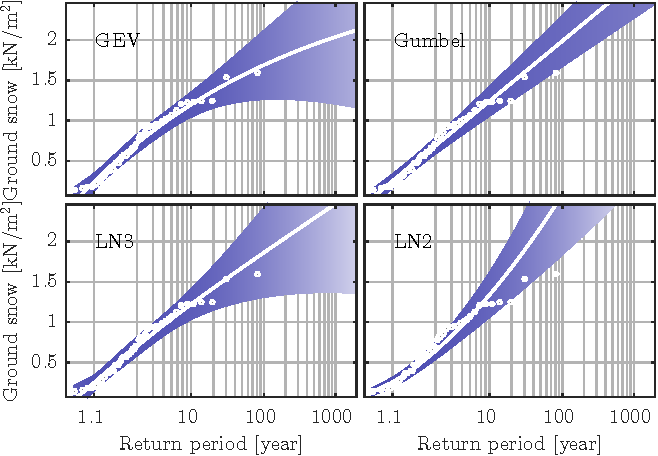
\includegraphics[]{filled_RP_RV_2x2_ID300_CI09.pdf}
	\caption{Location 1 (Weibull-like), ML fitted distributions with 90\% confidence bands (delta method) in Gumbel space.}
	\label{fig:loc1_2x2}
\end{figure}

\begin{figure}[htbp!]
	\centering    
	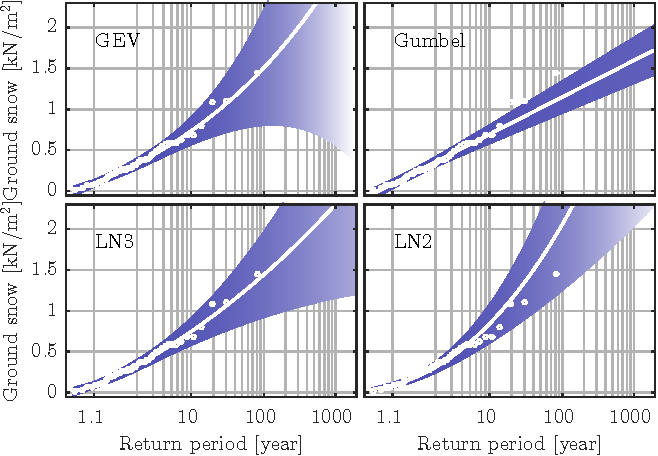
\includegraphics[]{filled_RP_RV_2x2_ID2735_CI09.pdf}
	\caption{Location 2 (Fréchet-like), ML fitted distributions with 90\% confidence bands (delta method) in Gumbel space.}
	\label{fig:loc2_2x2}
\end{figure}

\begin{figure}[htbp!]
	\centering    
	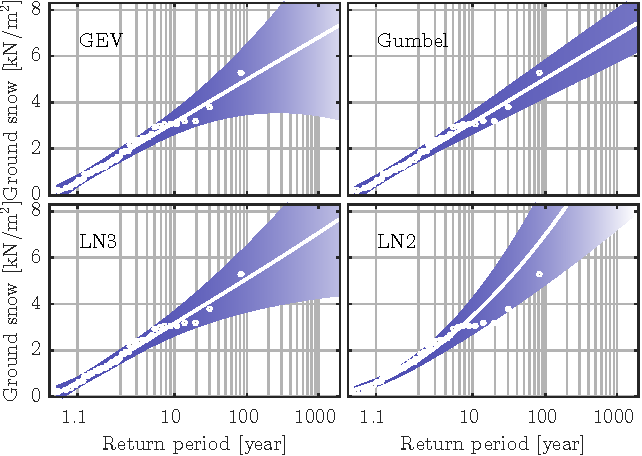
\includegraphics[]{filled_RP_RV_2x2_ID4553_CI09.pdf}
	\caption{Location 3 (Gumbel-like), ML fitted distributions with 90\% confidence bands (delta method) in Gumbel space.}
	\label{fig:loc3_2x2}
\end{figure}

All return value--return period plots -- with the exception of the Gumbel distribution -- show that the confidence interval is rapidly widening as the number of observations reduces and with extrapolation to unobserved region. This is especially salient for the Fréchet-like location (Figure~\ref{fig:loc2_2x2}). Figure~\ref{fig:loc3_2x2} indicates that even if the point estimates are similar, such as for GEV, Gumbel, and LN3, the confidence intervals can be substantially different in the extrapolated region. This information is completely lost if point estimates are considered only. Irrespectively of the location, the Gumbel distribution has significantly narrower confidence interval than the other models. This could be explained by its two parameters, which span smaller space.

By visual inspection the LN3 and GEV distributions seem to provide the best fit; however, in most cases their efficiency can hardly be proven by statistical and information theoretical methods, e.g. using Bayes weights (Eq.\ref{eq:bayes_weight}) or AICc (Eq.\ref{eq:AICc}). On the other hand, the narrow confidence interval of the Gumbel model is unjustified and can be critical in the case of Fréchet-like observations. For Weibull and Gumbel-like samples the LN2 model seems to considerably overestimate the fractiles when compared with the other models.

%....................................................................................
\subsection{Comparing representative fractiles}
To further illustrate the extent and effect of statistical uncertainties, four representative fractiles are inferred using the same four distributions and various methods presented in Chapter~\ref{cha:overview}. Return periods of 50, 100, 300 and 1000 years are selected. When these are interpreted as design point coordinates for the target reliability index of 3.8, then they correspond to sensitivity factors of 0.54, 0.61, 0.71 and 0.81, respectively. Thus, they are approximately representing structures with increasing susceptibility to snow loads; the former two may describe reinforced concrete and the latter two steel structures.

Point estimates with 90\% level uncertainty intervals for Location 1 and 2 are presented in Figures~\ref{fig:loc1_full_summary} and \ref{fig:loc2_full_summary}. The bootstrapping point estimate represents the mean as the mode cannot be estimated directly from the sample. Based on 10 bootstrappings the standard error is less than 1\% for LN2, LN3, and Gumbel distributions. It is about 7\% for large return periods of GEV distribution, which implies that GEV fractiles are more sensitive to sampling variability.

\begin{figure}[htbp!]
	\centering    
	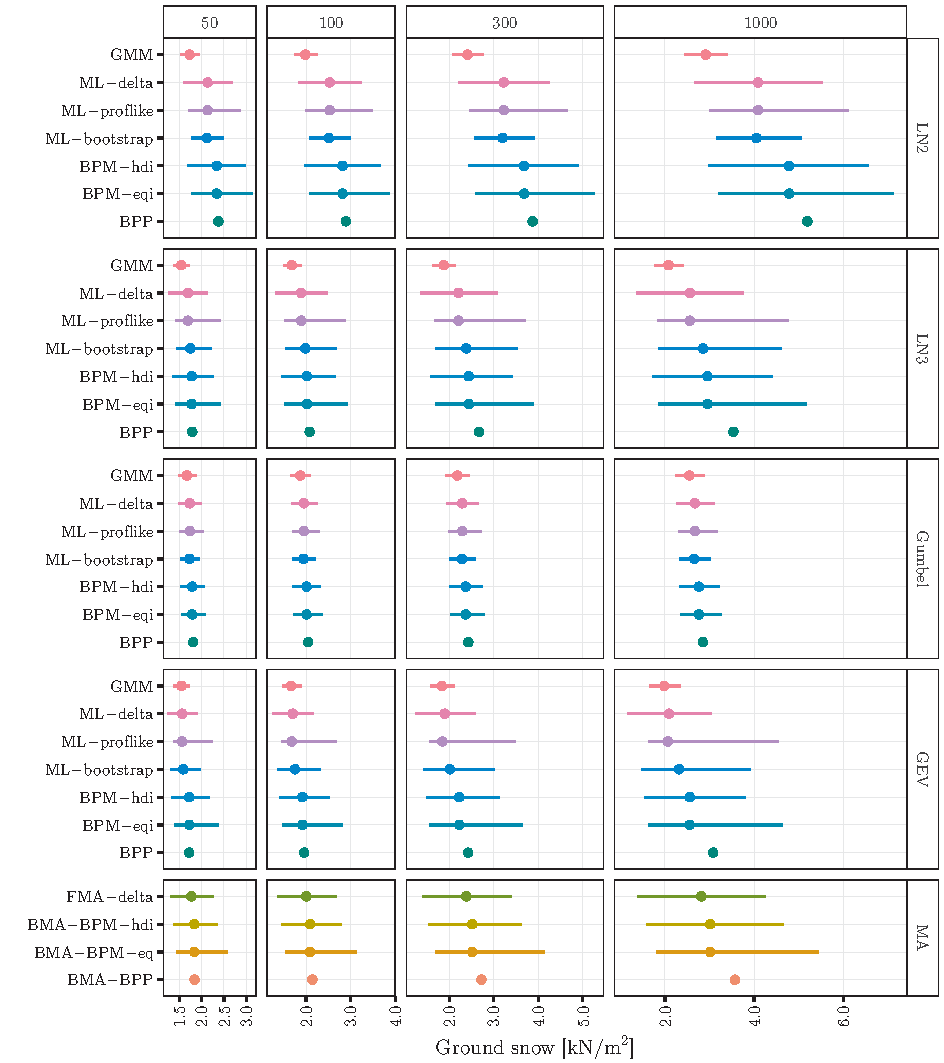
\includegraphics[]{ID300_full_summary_large.pdf}
	\caption{Location 1 (Weibull-like), summary of point estimates and 90\% level uncertainty intervals for the considered models, methods and return periods (notations are explained in Table~\ref{tab:stat_methods_notations}).}
	\label{fig:loc1_full_summary}
\end{figure}


\begin{figure}[htbp!]
	\centering    
	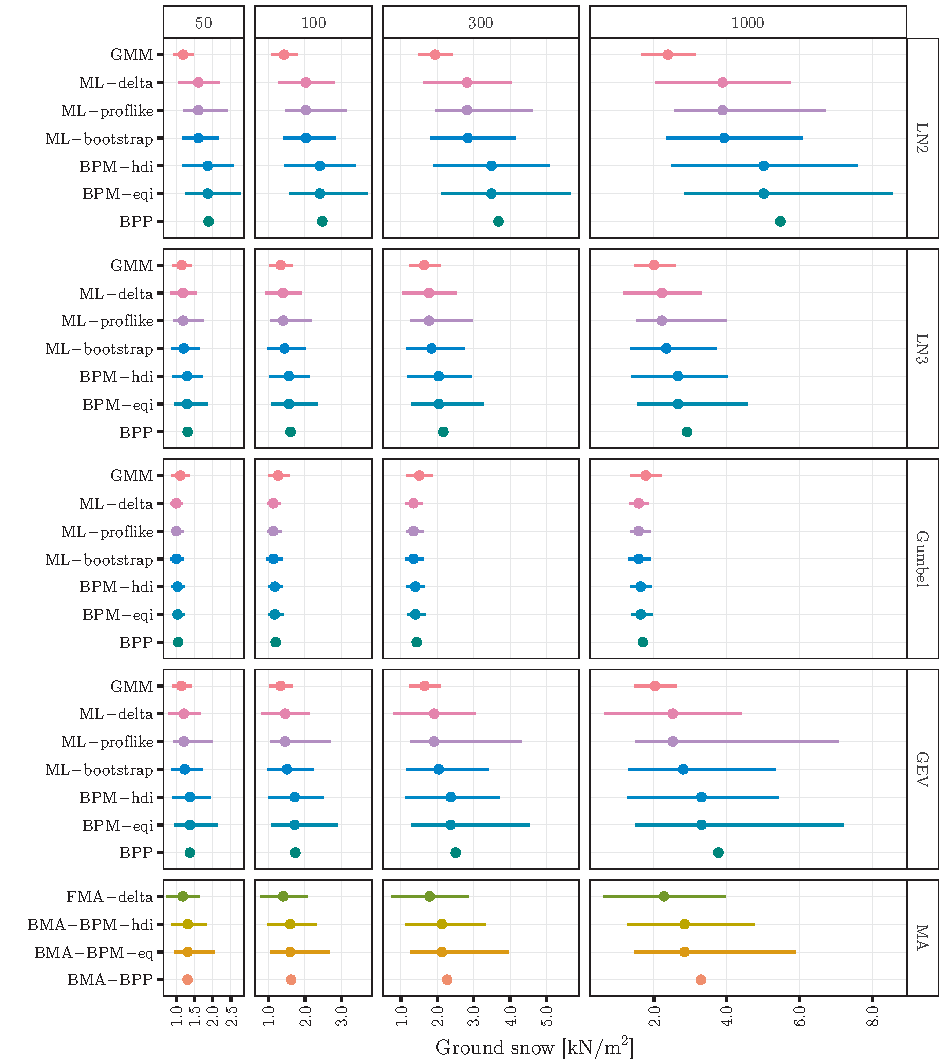
\includegraphics[]{ID2735_full_summary_large.pdf}
	\caption{Location 2 (Fréchet-like), summary of point estimates and 90\% level uncertainty intervals for the considered models, methods and return periods (notations are explained in Table~\ref{tab:stat_methods_notations}).}
	\label{fig:loc2_full_summary}
\end{figure}

For Location 1 the models show considerable difference even for the 50-year return period, for which the uncertainty intervals are relatively narrow. Compared with the Gumbel ML point estimate, the largest difference is observed for the Bayesian posterior predictive estimate of LN2 that is 1.4 times larger. The same ratios for 100, 300 and 1000-year return values are 1.5, 1.7 and 1.9, respectively. The uncertainty and the difference among point estimates for all the distributions become more significant with an increasing return period. The ML and Bayesian methods yield similar point estimates and comparable uncertainty intervals, the largest difference is observed for LN2. The GMM method gives smaller point estimates and narrower intervals than the other methods for Location 1, e.g. for LN3 it is 0.7-0.9 times smaller than the Bayesian posterior mean.

The results of comparative analyses for Location 2 are summarized in Figure~\ref{fig:loc2_full_summary}. This location shows similar trends as of Location 1, but here the difference between Gumbel and the other models increases, particularly in respect of uncertainty intervals.The 1000-year return values based on the LN2, LN3, and GEV models -- using the ML point estimates -- are 2.4, 1.4, 1.6 times larger than that of the Gumbel distribution. %The 1000-year fractile can be considered as the design point coordinate for lightweight steel structures \citep{Holicky2008}.

Besides the uncertainty intervals, the effect of parameter estimation uncertainty is quantified by the ratio of the corresponding posterior predictive and posterior mean fractiles (Table~\ref{tab:loc1_fract_ratio}). The numbers indicate that particularly for GEV and LN3 distributions the effect of this uncertainty becomes significant with increasing return periods. For these the neglect of parameter estimation uncertainty leads to 20\% underestimation of the return value.

\begin{table}[htbp!]
\caption{Location 1 (Weibull-like), ratio of the posterior predictive and posterior mean fractiles.}
\centering
\label{tab:loc1_fract_ratio}
\small
    \begin{tabular}{lllll}
    \toprule
    Return period [year]  & 50 & 100 & 300 & 1000 \\
    \midrule
    \rowcolor{lightgrey} LN2 & 1.02 & 1.03 & 1.05 &	1.09  \\
    LN3	& 1.01 & 1.03 &	1.10 & 1.20  \\
    \rowcolor{lightgrey} Gumbel & 1.01 & 1.02 &	1.02 & 1.03  \\
    GEV & 1.00 & 1.02 &	1.09 &	1.20  \\
   	\rowcolor{lightgrey} BMA & 1.00 & 1.02 &	1.08 & 1.18 \\
    \bottomrule
    \end{tabular}
\end{table}

Return period estimates are compared for models with and without parameter estimation uncertainty in Table~\ref{tab:loc1_reper}. For LN3 and GEV posterior predictive distributions, the return periods are half of those of the posterior mean distributions. The sampling variability has considerable effect on these values, hence they should be treated as indicative.

\begin{table}[htbp!]
\caption{Location 1 (Weibull-like), return periods, derived from posterior predictive distributions corresponding to 1000-year fractiles based on matching posterior mean distributions.}
\centering
\label{tab:loc1_reper}
\small
    \begin{tabular}{lllll}
    \toprule
    Distribution  & LN2 & LN3 & Gumbel & GEV \\
    \midrule
    \rowcolor{lightgrey} Return period & 704 & 436 & 779 &	413  \\
    \bottomrule
    \end{tabular}
\end{table}

The results (Table~\ref{tab:loc1_fract_ratio} and Figure~\ref{fig:loc1_full_summary}-\ref{fig:loc2_full_summary}) show that the distribution type has larger effect on the representative fractiles than the parameter estimation uncertainty. For example for Location 2 the ratios of the 1000-year fractile of the posterior predictive and posterior mean models are 1.09, 1.09, 1.03, 1.14 and 1.16 for LN2, LN3, Gumbel, GEV and MA models respectively. These illustrate the effect of parameter estimation uncertainty.

The model selection uncertainty can be assessed by comparing the posterior mean fractiles for different models. Normalizing the 1000-year fractile of posterior mean models with that of the Gumbel the ratios are 3.05, 1.62, 1.00, 2.01 and 1.73 for LN2, LN3, Gumbel, GEV and MA (model averaged) models respectively. For other locations the trend is similar but less pronounced.

%.......................................................................................
\subsection{Model averaging}
Figures~\ref{fig:loc1_full_summary} and \ref{fig:loc2_full_summary} show that the frequentist (FMA) and Bayesian (BMA) model averaged point and interval estimates yield comparable results, although the frequentist fractiles and intervals tend to be smaller. A more detailed exposition of model averaging of the Bayesian posterior marginals of the fractiles is illustrated in Figure~\ref{fig:loc1_posterior_bma_2x2}. For larger return periods the difference among the models is increasing, thus the model averaged distribution might become multimodal. For Location 1, the Akaike weights are 0.19, 0.20, 0.43 and 0.18 for LN2, LN3, Gumbel, and GEV distributions, respectively. The Bayesian weights given in the same order are 0.13, 0.29, 0.30 and 0.28.

Model averaging certainly provides a better fit than any of the individual models, but since it typically requires considerable additional computational efforts, it is recommended mainly for critical structures and extreme hazards such as nuclear facilities and discharges, rather than common applications.

\begin{figure}[htbp!]
	\centering    
	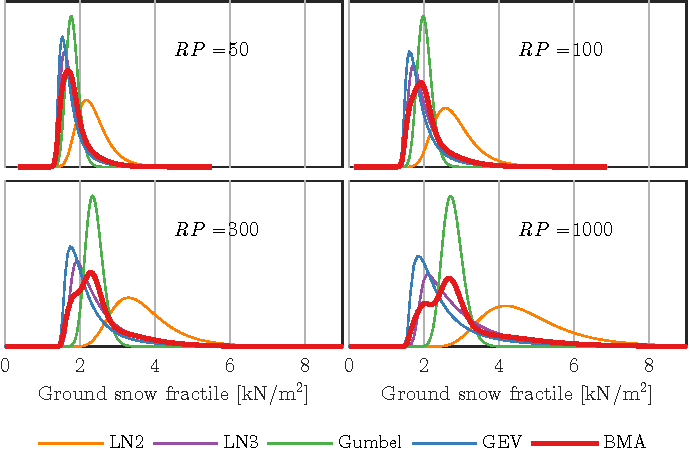
\includegraphics[]{posterior_BMA_2x2_ID300.pdf}
	\caption{Location 1 (Weibull-like), posterior distributions of selected fractiles per different distribution types and Bayesian model averaging.}
	\label{fig:loc1_posterior_bma_2x2}
\end{figure}


%****************************************************************************************
%***************************************************************************************
\section{Effect on structural reliability}
From a practical viewpoint the reliability index is often a more interesting parameter than representative fractiles. Thus the aim of this section is to investigate the effect of statistical uncertainties on structural reliability and to provide practical recommendations regarding their treatment. For this purpose, the reliability level of a generic structural member subjected to snow load is investigated. The effect of parameter estimation and model selection uncertainty in ground snow maxima is considered using frequentist and Bayesian techniques. In contrast with the typically used fixed model and ``best'' point estimates, model averaging and uncertainty intervals are used respectively.

%****************************************************************************************
\subsection{Conceptual framework}
To study the effect of statistical uncertainties, two sets of mechanical-probabilistic models with different representation of the ground snow load are compared. These two model sets are referred hereinafter as \textit{analyzed} and \textit{reference models}, and they differ solely in the ground snow distribution. For example, to illustrate the effect of parameter estimation uncertainty, the \textit{reference model} contains the posterior mean distribution while the \textit{analyzed model} uses the posterior predictive distribution of ground snow. The \textit{reference model} is used to find a mean value of the resistance to reach the target reliability level, which is selected as 3.8 for a considered 50-year reference period. The \textit{analyzed model} has the same mean resistance and thus results based on this model show the effect of different ground snow representation. Throughout this section, different \textit{analyzed-reference model} pairs are considered to illustrate various effects.

The ground snow data of Budapest are used for the analyses (Location 4 in Table~\ref{tab:loc_parmest}). This location  represents lowland areas in the Carpathian Region. Annual maxima from 49 winter seasons are extracted to infer the distributions.

%****************************************************************************************
\subsection{Mechanical and probabilistic model} 

The mechanical model and loads of the analyzed structural member are presented in Figure~\ref{fig:beam_illustration}. The flexural failure of a mid-span cross-section is selected as a representative ultimate limit state:
\begin{equation}
%	\label{eq:BMA}
	g(\mathbf{X}) = {K_{\mathrm{R}}} \cdot R - {K_{\mathrm{E}}} \cdot \left( {\mu  \cdot {s_{{\mathrm{g,50}}}} + {g_{\mathrm{p}}}} \right) \cdot a \cdot \frac{{{L^2}}}{8}.
\end{equation}

\begin{figure}[htbp!]
	\centering    
	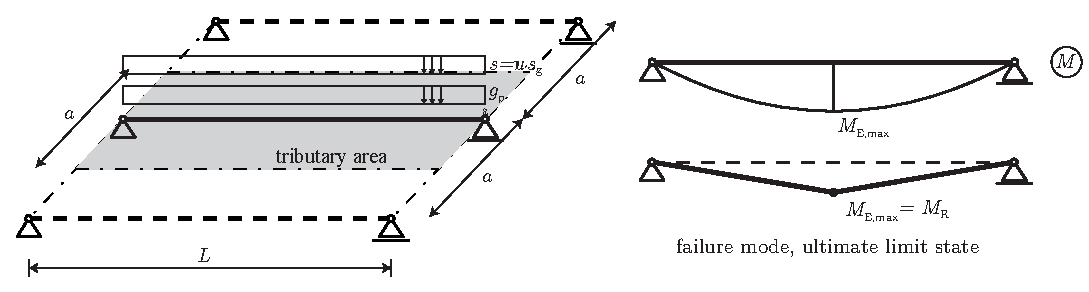
\includegraphics[width = 1\textwidth]{beam_illustration.pdf}
	\caption{Illustration of the analyzed structural member and its failure mode.}
	\label{fig:beam_illustration}
\end{figure}

The variables with their probabilistic model are given in Table~\ref{tab:prob_model_IABSE}. For the annual ground snow load ($s_\mathrm{g,1}$) the sample mean and coefficient of variation ($CV$) are provided since these are also dependent on the fitted distribution type and technique applied to infer parameters of a distribution. The skewness of the analyzed sample is 1.6, indicating Fréchet-type distribution family (Figure~\ref{fig:gev_skewness}). The commonly used Gumbel, Generalized extreme value, two-parameter Lognormal, and three-parameter Lognormal distributions are applied to represent the annual ground snow maxima. The connection between the 1-year and 50-year maxima distributions is established by assuming that the annual maxima are mutually independent.

\begin{table}[htbp!]
\caption{Probabilistic models of simple beam example.}
\centering
\label{tab:prob_model_IABSE}
\small
	\begin{threeparttable}
    \begin{tabular}{l l l l m{3cm}}
    \toprule
    Variable name  & Distribution & Mean & CV & Reference \\
    \midrule
    \rowcolor{lightgrey} Resistance model uncertainty, $K_\mathrm{R}$ [-]  & LN2 & 1.00 & 0.10 & \cite{JCSS_resi} \\
    Resistance, $R$ [kNm] & LN2 & \tnote{*} & 0.15 & \cite{JCSS_resi} \\
    \rowcolor{lightgrey} Load model uncertainty, $K_\mathrm{E}$ [-] & LN2 & 1.00 & 0.10 & \cite{JCSS_load} \\
    Shape factor, $\mu$ [-] & LN2 & 0.80 & 0.17 & \cite{Ellingwood1985} \\
    \rowcolor{lightgrey} Ground snow load, $s_\mathrm{g,1}$ [kN/m$^2$] & \tnote{\textdagger} & 0.4\tnote{\ddag} & 0.7\tnote{\ddag} & \cite{Szalai2013} \\
    Permanent load, $g_\mathrm{p}$ [kN/m$^2$] & N & \tnote{\S} & 0.10 & \cite{JCSS_load} \\
    \rowcolor{lightgrey} Beam span, $L$ [m] & -- & 10 & -- & -- \\
     Bay distance, $a$ [m] & -- & 3 & -- & -- \\
    \bottomrule
    \end{tabular}
    \begin{tablenotes}
    	\item[*] Based on FORM analysis to reach $\beta_\mathrm{target} = 3.8$ with a fixed coefficient of variation.
	    \item[\textdagger] Gumbel, GEV, LN2, LN3, see Appendix~\ref{sec:distr_fun}.
	    \item[\ddag] Using unbiased moment estimates of the sample.
	    \item[\S] Varied to get different load ratios $(\chi)$.
	    \item -- Not applicable/not available.
   	\end{tablenotes}
   	\end{threeparttable}
\end{table}

Different load ratios are achieved by varying the mean value of the permanent load while keeping its coefficient of variation fixed. The load ratio is defined as:
\begin{equation}
	\label{eq:load_ratio}
	\chi  = \frac{{{\mu _{\mathrm{m}}} \cdot {s_{{\mathrm{g,k}}}}}}{{{\mu _{\mathrm{m}}} \cdot {s_{{\mathrm{g,k}}}} + {g_{\mathrm{m}}}}}
\end{equation}
where the m and k subscripts refer to mean and characteristic values respectively.

%****************************************************************************************
\subsection{Statistical analysis}
Frequentist and Bayesian statistical techniques are applied to fit models to the snow maxima and to quantify statistical uncertainties. For the current analysis their most important difference is that the Bayesian approach treats parameters as random variables, thus makes it possible to integrate their estimation uncertainties into the failure probability.

Maximum likelihood and posterior mean are used as point estimates per frequentist and Bayesian approaches respectively. Accordingly, the distributions specified by these point estimates are referred to as maximum likelihood and posterior mean distributions (Table~\ref{tab:stat_methods_notations}).

For the Bayesian calculations vague priors are applied for both to the parameters and to the models as well, and numerical integration is used to calculate the posterior and posterior predictive distributions. Practically infinite ranges are selected for the integrations and uniform priors are adopted on these intervals.

%.......................................................................................
\subsubsection{Results of distribution fitting}
The statistical uncertainties of ground snow models are illustrated on return value-return period plots with confidence bands (Figure~\ref{fig:2546_rp_rv_2x2}). The solid white lines and blue regions show the ML point estimates and 90\% confidence bands respectively; the latter illustrates the parameter estimation uncertainty. The dashed white line and green region correspond to the FMA point estimate and 90\% confidence bands respectively. The extent of model selection uncertainty can be judged by comparing the blue regions to the green ones. For example, for the Gumbel distribution the blue region is considerably wider than the green, this implies that the Gumbel confidence interval is too narrow. This is also supported by the evidence that maxima of the sample are outside of the 90\% confidence band (Figure~\ref{fig:2546_rp_rv_2x2}). This can be observed also for other locations from the CarpatClim database with skewness exceeding 1.2.

\begin{figure}[htbp!]
	\centering    
	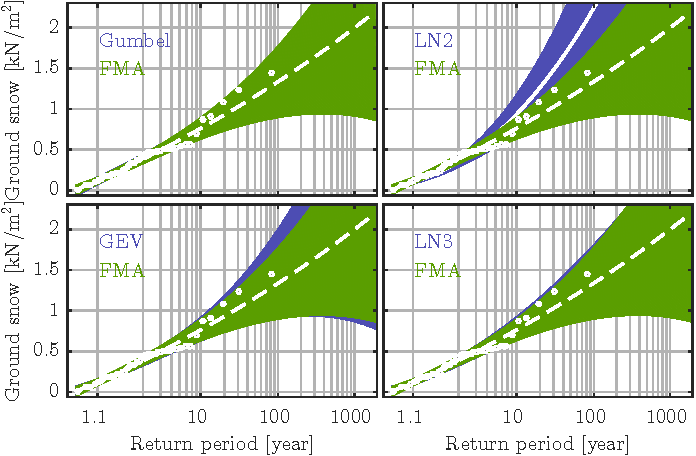
\includegraphics[]{filled_RP_RV_2x2_FMA_ID2546_CI09.pdf}
	\caption{Annual maxima return value--return period plots with 90\% confidence bands for the selected (blue + solid white) and FMA (green + dashed white) distributions in Gumbel space.}
	\label{fig:2546_rp_rv_2x2}
\end{figure}

The Bayesian analysis yields to similar results as the frequentist, although the averaging weights are slightly favoring the three-parameter models over the two-parameter ones (Table~\ref{tab:ma_weights}). Both methods indicate that there is a strong evidence against the LN2 model for this location.

\begin{table}[htbp!]
\caption{Summary of model averaging weights.}
\centering
\label{tab:ma_weights}
\small
    \begin{tabular}{lll}
    \toprule
    Model  & Akaike weight, $w$ & Bayesian weight, $b$ \\
    \midrule
    \rowcolor{lightgrey} GEV  & 0.29 & 0.37 \\
    Gumbel  & 0.43 & 0.25 \\
    \rowcolor{lightgrey} LN3  & 0.28 & 0.38 \\
    LN2  & 0.004 & 0.002 \\
    \bottomrule
    \end{tabular}
\end{table}

Table~\ref{tab:char_snow_bp} shows the characteristic values (0.98 fractile) for the considered models and statistical approaches. With the exception of LN2, which is not supported by the data, the models yield to comparable values. Due to parameter estimation uncertainty the largest increase is observed for LN3, it is about 8\%. The Gumbel model underestimates the model averaged characteristic value by about 10\%. The results for this location are in good agreement with the 1.25 kN/m$^2$ characteristic value specified in the Hungarian National Annex of EN 1991-1-3.

\begin{table}[htbp!]
\caption{Summary of ground snow load characteristic values for Budapest [kN/m$^2$].}
\centering
\label{tab:char_snow_bp}
\small
	\begin{threeparttable}
    \begin{tabular}{l p{3cm} p{3cm} p{3cm}}
    \toprule
    Distribution  & Maximum likelihood (ML) & Bayesian posterior mean (BPM) & Bayesian posterior predictive (BPM) \\
    \midrule
    \rowcolor{lightgrey} GEV  & 1.23 & 1.34 & 1.38  \\
    Gumbel  & 1.07 & 1.11 & 1.12  \\
    \rowcolor{lightgrey} LN3  & 1.20 & 1.18 & 1.28  \\
    LN2  & 1.78 & 1.90 & 1.98  \\
    \rowcolor{lightgrey} FMA & 1.16 & -- & --  \\
   	BMA  & -- & 1.21 & 1.27 \\
    \bottomrule
    \end{tabular}
    \begin{tablenotes}
    	\item -- Not applicable.
    \end{tablenotes}
    \end{threeparttable}
\end{table}

%****************************************************************************************
\subsection{Reliability analysis}

Reliability of the selected structural member is analyzed using the first order reliability method (FORM) considering the various probabilistic representation of the ground snow maxima. Initially a commonly applied Gumbel distribution is investigated. The \textit{reference model} is the Gumbel maximum likelihood distribution, while the analyzed models are the four selected maximum likelihood and the frequentist model averaged distributions. The reliability indices with approximate 90\% confidence bands are presented in Figure~\ref{fig:beta_khi_fma_2x2}. These bands express solely the statistical uncertainties in the ground snow distributions.

This analysis represents the following scenario: Gumbel ML distribution is adopted for snow maxima and a structural member is designed to achieve the target reliability. The failure probability is then calculated assuming that the snow maxima follows other distributions. Figure~\ref{fig:beta_khi_fma_2x2} shows the followings:
\begin{itemize}
	\item The distribution type has substantial effect on the reliability, e.g. for large load ratios the GEV model yields to about 50 times larger failure probability than the Gumbel.
	\item All models yield to smaller reliability index than the \textit{reference} Gumbel.
	\item Compared to the FMA model, the failure probability and uncertainty intervals are largely underestimated by the Gumbel model.
\end{itemize}

\begin{figure}[htbp!]
	\centering    
	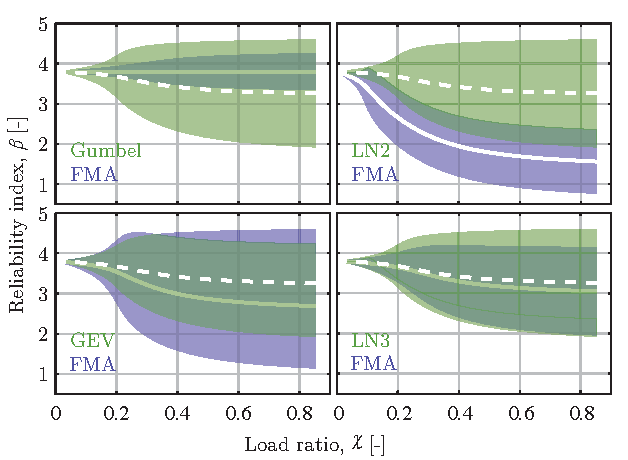
\includegraphics[]{khi_beta_2x2_FMA_ID2546_CI09.pdf}
	\caption{Load ratio–-reliability index plots with 90\% confidence bands for the selected (green + solid white) and FMA (blue + dashed white) ground snow distributions, using Gumbel ML as \textit{reference model}.}
	\label{fig:beta_khi_fma_2x2}
\end{figure}

As the LN2 model is clearly far from the FMA, and not supported by the data (Table~\ref{tab:ma_weights}), it is discarded from the following analyses. The same analysis with BPM models yields to similar results as those of the maximum likelihood based. Since the Bayes weights favor the GEV and LN3 models, the underestimation of Gumbel model is even larger than in the case of FMA.

Figure~\ref{fig:beta_khi_bma_2x2} shows the effect of statistical uncertainties, here the \textit{reference model} is the BPM for each selected model, hence the solid green line is horizontal, indicating the 3.8 value. The \textit{analyzed models} are the BPP and BMA models. The main observations from Figure~\ref{fig:beta_khi_bma_2x2} are as follows:
\begin{itemize}
	\item The effect of parameter estimation uncertainty within the Gumbel model is small; however, the model uncertainty has substantial effect, significantly exceeding an order of magnitude in failure probability.
	\item For GEV and LN3 the consideration of parameter estimation uncertainty gives about 20 and 5 times larger failure probability, respectively.
	\item These effects are rapidly increasing with increasing load ratio and reaching a relatively stable level after ratio of 0.3.
\end{itemize}


\begin{figure}[htbp!]
	\centering    
	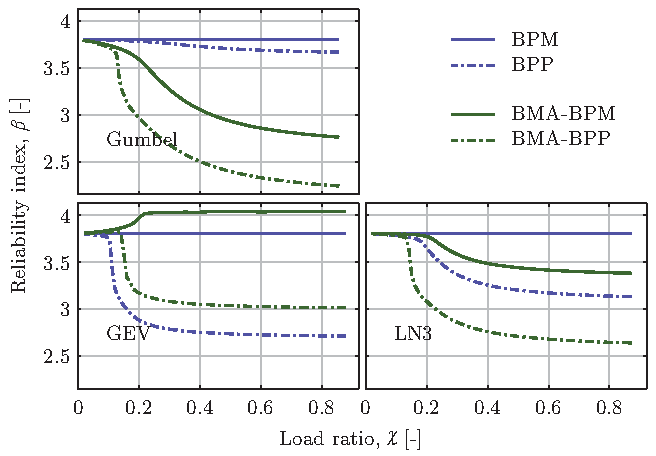
\includegraphics[]{khi_beta_2x2_BPM_BPP_BMA_ID2546_CI09_02.pdf}
	\caption{Load ratio–-reliability index plots for models with (dash-dot) and without parameter estimation uncertainty (solid).}
	\label{fig:beta_khi_bma_2x2}
\end{figure}

Although Table~\ref{tab:char_snow_bp} indicates only minor differences in the characteristic values for the selected probabilistic models, the reliability indices in Figure~\ref{fig:beta_khi_bma_2x2} suggest that the model selection is a key issue for reliability analysis. Consequently, comparison of characteristic values seems to be insufficient to support decision about appropriate probabilistic model.

%\subsection{Extension}

% reference to not detailed works
%75\% confidence interval estimate
%identification of most important component with largest contribution
%\citep{RozsasTVSB2015}


%****************************************************************************************
%****************************************************************************************
\section{Application example: Eiffel-hall of Budapest}

The Eiffel-hall of Budapest is selected to demonstrate the effect of statistical uncertainties on a real life example. The structure is introduced in Annex~\ref{sec:eiffel}, here only the essential details, which are required to interpret the results, are provided. Maximum likelihood method is applied to infer the parameters of annual ground snow maxima of the site. Two-parameter Lognormal, three-parameter Lognormal, Gumbel, and Generalized extreme value distributions are considered for the analysis. The results in terms of reliability indices and normalized failure probabilities are given in Table~\ref{tab:eiffel_statunc}. 50-year reference period is used for all calculations of the structure.

\begin{table}[htbp!]
\caption{Summary of the reliability measures of the selected purlin.}
\centering
\label{tab:eiffel_statunc}
\small
    \begin{tabular}{lllll}
    \toprule
      & Gumbel & GEV & LN2 & LN3 \\
    \midrule
    \rowcolor{lightgrey} $\beta$ & 3.27  & 2.88 & 1.42 & 2.86 \\
    $P_\mathrm{f}/P_\mathrm{f,Gumbel}$ & 1.00  & 3.68 & 145 & 3.96 \\
    \bottomrule
    \end{tabular}
\end{table}

As the site has Fréchet-like distribution with shape parameter greater than zero, all models yield to larger failure probability than that of the Gumbel. The LN3 and GEV failure probabilities are similar and four times larger than that of the Gumbel. The underestimation of Gumbel distribution is more salient for the LN2 distribution that leads to two order of magnitude difference and well represents the significant effect of model selection uncertainty.

%****************************************************************************************
%****************************************************************************************
\section{Discussion}

The main focus of this chapter is the quantification and propagation of statistical uncertainties. From a broader engineering perspective that views reliability analysis as a tool for decision making, the model selection uncertainty problem is recommended to be resolved by agreeing on a conventional distribution type \citep{Melchers2002, Ditlevsen1994}. We support this approach; however, the decision on the selected distribution should be backed by appropriate techniques for model uncertainty analysis. For safety-critical facilities and actions it still might be desirable to analyze this source of uncertainty in detail. The Generalized extreme value distribution is recommended to represent annual maxima of ground snow extremes.This is not a novel recommendation as multiple studies considered GEV or members of GEV family, but for standardization they often settled with other types \citep{Sanpaolesi1998, Ellingwood1984}.

Regarding parameter estimation uncertainty it is argued that it is often advisable to be considered in reliability studies by using the posterior predictive distribution. The main arguments are that reliability analysis is inherently predictive, the failure probability is governed by the very uncertain distribution tails, and after the selection of distribution function it is unambiguous to construct the posterior predictive estimates.
The presented uncertainty interval construction techniques require no or several additional limit state function evaluations as compared to the standard reliability methods such as FORM, and thus are applicable to complex problems as well.

It is argued that in structural reliability every random variable should be represented by its posterior  predictive distribution and for critical cases model averaging should be adopted. This is not a novel in-sight, treatment of statistical uncertainties is well developed in the statistical literature \citep{Wit2012, Aitchison1980} and also advocated in relation to probabilistic engineering analysis \citep{Kiureghian2008, Coles2003fully_prob, Gelder2000}.

The treatment of uncertainties is always related to the  considered  ``model universe'',  i.e.  the  physical and mathematical framework (model) adopted to describe  the  reality.
If point estimates are used the models derived from 5 realizations would convey the same confidence as those based on 1000 data. In contrast, the Bayesian posterior predictive distribution automatically penalizes the small sample size based predictions.
Both presented model averaging (MA) techniques depend on the considered models (the weights in Eq.\ref{eq:bayes_weight}), thus can be interpreted only in respect of the space of selected models.

It should be noted that the results are based on the analysis of few locations with fixed number of observations. For other phenomenon, such as wind extremes, which are typically following Weibull distribution, the effects are anticipated to be smaller. However, smaller number of observations can considerably increase statistical uncertainties. Moreover, it is expected that these uncertainties can be reduced by taking into account more informative priors, which are often available. 

To support future snow maxima related studies the posterior distributions of GEV parameters related to lowlands, and mountains and highlands of the Carpathian Region are calculated and given in Annex~\ref{sec:GEV_posterior}. These can be used as prior information for regions with similar climatic conditions.


%%****************************************************************************************
%%****************************************************************************************
%%\section{Extension to other random variables}
%
%Statistical uncertainties are present for all random variables because they are also inferred from limited observations. The same analysis could be repeated with different distribution types, coefficient of variations or incorporating statistical uncertainties of more random variables.
%\begin{itemize}
%	\item crucial random variables can be identified, e.g. consideration of statistical uncertainties is more important for variable actions than for resistance variables; for wind action, which follows Weibull distribution and has lower coefficient variation than snow loads the effect is less pronounced, for seismic actions it can be even more crucial due to large coefficient of variation \citep{Ellingwood2001}.
%	\item it is valuable if the findings are generalized and extended to other random variables, since the same problems occur.
%\end{itemize}
%
%extensive, at first high quality wind data is available for the Netherlands
%http://www.r-bloggers.com/wind-in-netherlands/


%****************************************************************************************
%****************************************************************************************
\section{Summary and conclusions}

The current practice in civil engineering prevalently overlooks parameter estimation and model selection uncertainties in probabilistic calculations. To assess the effect of this simplification frequentist and Bayesian statistics along with reliability analyses are utilized and the following conclusions are drawn:

\begin{itemize}
	\item The effect of parameter estimation uncertainty within the Gumbel model is small; however, the model uncertainty has substantial effect, considerably exceeding an order of magnitude in failure probability.
	\item The distribution choice may lead to 50 times increase in failure probability (GEV vs. Gumbel).
	\item For the Generalized extreme value and three-parameter Lognormal distributions the consideration of parameter estimation uncertainty can yield to about 20 and 5 times increase in failure probability, respectively.
	\item The use of ``best'' point estimates such as maximum likelihood estimator is not conservative and can have practically significant effect on calculated failure probability.
\end{itemize}

The following practical recommendations and observations are made based on completed analyses:

\noindent For common structures and standardization:
\begin{itemize}
	\item Consensus on the conventional distribution type is needed.  
	\item The commonly applied Gumbel model for annual maxima is often inadequate, this means that it underestimates failure probability and has deceptively narrow uncertainty interval, this model assumption should be revisited.  
	\item Bayesian approach is recommended to handle parameter estimation uncertainties.
\end{itemize}

\noindent For structures that require fully probabilistic risk assessment framework:
\begin{itemize}  
	\item Bayesian statistics is promoted to incorporate both model selection and parameter estimation uncertainties.  
	\item Generalized extreme value distribution is recommended for probabilistic modeling of extremes.
	\item Inclusion of all available data and prior information is recommended; however, guidance on priors is needed.
\end{itemize} 

The consideration of statistical uncertainties can be especially important for predicting extremes under changing climate for which one cannot rely on historical observations.

%The adopted techniques are not restricted to the considered problem and can be utilized for other random variables, phenomena as well, e.g. floods and wind loads.
 
%The applied distribution type has a larger effect on representative fractiles than the parameter estimation uncertainty. Numerical analysis of the annual maxima of ground snow loads reveals that the Gumbel distribution provides unrealistically narrow uncertainty intervals. Use of the generalised extreme value distribution is recommended. The applied parameter estimation technique has considerable effect on the representative fractiles.

%The effect of available observations:
%wind speed study \cite{RozsasREC2016wind}
%stochastic process \ref{cha:copula}
%problems of adaptation and comparison

%The current Eurocode provisions yield to insufficient reliability level if these uncertainties are incorporated, the difference is increasing with increasing snow to dead load ratio.
\chapter{Effect of measurement uncertainty}
\label{cha:error}
% **************************** Define Graphics Path **************************
\ifpdf
    \graphicspath{{Chapter4/Figs/Raster/}{Chapter4/Figs/PDF/}{Chapter4/Figs/}}
\else
    \graphicspath{{Chapter4/Figs/Vector/}{Chapter4/Figs/}}
\fi

% **************************** Chapter Abstract ******************************
\leftskip=1cm
\noindent
\emph{Observations are inevitably contaminated with measurement uncertainty, which is a predominant source of uncertainty in some cases. In reliability analysis, probabilistic models are typically fitted to measurements without considering this uncertainty. Hence, this chapter intends to explore the effect of this simplification on structural reliability and to provide recommendations on its treatment. Statistical and interval-based approaches are used to quantify and to propagate measurement uncertainty. They are critically compared by analyzing ground snow measurements, which are often affected by large measurement uncertainty. It is propagated through the mechanical model of a generic structure to investigate its effect on reliability. 
%Parametric studies facilitate to analyze the effect of key parameters, such as measurement uncertainty, coefficient of variation of ground snow load, and distribution type. The interval analysis is performed as a hybrid interval-probabilistic analysis. Measurements are represented as intervals and probabilistic model is then fitted to them. Thus, snow parameters and the reliability index are also interval variables; other random variables are described by standard probabilistic distributions. Implementation of the statistical approach is based on the frequentist paradigm where the contamination mechanism is expressed in terms of random variables. This approach allows decoupling measurement uncertainty from a variable of interest.
The results indicate that measurement uncertainty may lead to significant (order of magnitude) underestimation of failure probability and should be taken into account in reliability analysis. 
%If more information than interval endpoints is available, a statistical approach is recommended; otherwise the interval representation should be used.
Ranges of the key parameters are identified where measurement uncertainty should be considered. For practical applications, the lower interval bound and predictive reliability index are recommended as point estimates using interval and statistical analysis, respectively. The point estimates should be accompanied by uncertainty intervals, which convey valuable information about the credibility of results. 
%Although general recommendations are given, treatment of measurement uncertainty should be handled on a case-specific basis.
}

\leftskip=0pt\rightskip=0pt

%****************************************************************************************
%****************************************************************************************
\section{Problem statement and the state of the art}

Models accounting for all uncertainties are of a considerable interest in structural reliability since these are the bases of design specifications, hence impacting the building and structure stocks of large regions. Snow is particularly important for light-weight structures for which it is typically the governing action. To our knowledge, the effect of snow measurement uncertainty on structural reliability has not yet been studied and other probabilistic models are treated similarly in civil engineering. For instance, neither the joint European research on snow actions \citep{Sanpaolesi1998} or the JCSS Probabilistic Model Code \citep{JCSS_basis} provides any information on the treatment of measurement uncertainty and its effect. Therefore, the aim of this chapter is to explore the effect of this simplification on structural reliability and to provide recommendations on its treatment.

Observations are inevitably contaminated with measurement uncertainty (MU), which is a predominant source of uncertainty in some cases. Uncertainty is understood here as the lack of knowledge (epistemic) and natural variability (aleatory)\footnote{This division is subjective as conditioned on the selected ``model universe''.}  not including known systematic error, which are assumed to be adjusted. In reliability analysis, probabilistic models are typically fitted to measurements without considering their uncertainty. This is the case for snow measurements where often only the snow depth is measured and the applied techniques makes the derived loads highly uncertain, for example, the uncertainty range can reach 50\% of the measured depth\footnote{Based on a personal correspondence with a meteorologist.}. 

The World Meteorological Organization conducted a comprehensive comparative study on the then available solid precipitation measurement techniques and experimentally confirmed that measurements should be adjusted for wetting loss, evaporation loss, and wind induced undercatch \citep{Goodison1998}. They found that the snow catch ratio of the four most widely used gauges ranges from 20\% to 70\% at 6 m/s wind speed. Even for automated systems, measurement error in solid precipitation can vary from 20\% to 50\% due to undercatch in windy conditions \citep{Rasmussen2012}. Although these mainly contribute to systematic error they indicate uncertainties in snow measurements as these errors cannot be exactly corrected. For instance coefficient of determination ($R^2$) values vary from 0.40 to 0.80 for the fitted wind correction equations at certain sites; these are associated with about 10\% standard error in catchment ratio. Additional uncertainty may be introduced if no site specific auxiliary data, e.g. wind speed measurements, are available \citep{Goodison1998}. These issues are not limited to snow measurements but valid for all evidence based models -- that is for every model -- although their importance may vary.

%****************************************************************************************
%****************************************************************************************
\section{Solution strategy}
%*****************************************************************************************
\subsection{Adopted approaches}

We assume that measurements are corrected for known systematic errors. Additionally, the following model is assumed to describe the connection between observed ($Y$) and real, true, physical ($X$) values, i.e. the variable of interest:
\begin{equation}
\label{eq:ro_link}
	\mathrm{(true, real\footnotemark)} X \xrightarrow[]{h(X,E)} Y \mathrm{(observed)}.
\end{equation}
\footnotetext{Herein we tacitly assume the existence of some objective reality independent of the observer.}
The $h(X, E)$ function represents the mathematical relationship between the true and observed random variables referred hereinafter as reality-observation link. $E$ covers the unknown processes contributing to measurement uncertainty. The recommended probabilistic models -- typically distributions -- in the literature are almost exclusively given for the true variable and not for the observed, potentially contaminated one. Possible reasons for this are that:
\begin{itemize}
	\item The contamination is commonly site- and measuring technique-dependent, thus no general recommendations can be given for the distribution of $Y$.
	\item The model type is often selected based on theoretical arguments considering the physical phenomena generating $X$, for example Normal distribution if $X$ is the result of summation; Lognormal if $X$ is the product of random variables; extreme value distribution if $X$ is related to extremes.
	\item Structural reliability ultimately depends on $X$ and not on $Y$, although we are limited to access only $Y$.
\end{itemize}

The last point is especially important since structures are subjected to actions coming from $X$ and not from $Y$; the latter is affected by our ignorance or inability to make accurate measurements (epistemic uncertainty). In a broader sense this also applies for $X$, but for now we remain in the commonly accepted model universe of engineering and treat $X$ as a random variable. If the distribution type of $X$ is known or agreed, then the reality-observation link uniquely determines the distribution of $Y$. Hence, if any measurement uncertainty is present, its distribution type almost certainly differs from the distribution of $X$. This is prevalently neglected while fitting distributions in civil engineering -- $Y$ is assumed to be distributed as $X$. This simplification is acceptable in some practical cases. This method is termed hereinafter as Approach~1 while it is referred to as Approach~2 when the difference between distributions is appreciated:
\begin{description}
	\item[Approach~1] Use the probabilistic model of true random variable ($X$) and treat the observations -- contaminated with measurement uncertainty -- ($\mathbf{y}$) as the realizations of this model: $\mathbf{y} \sim X$.
	\item[Approach~2] Differentiate between the distribution of true and observed random variables. Within this, the following two sub-approaches are considered:
	\begin{description}
		\item[Approach~2a] Representation of measurement uncertainty with intervals at the level of observations and propagating them to the derived parameters via interval analysis. As interval representation by nature contains no information about the reality-observation link, the decontamination of observations is not possible.
		\item[Approach~2b] Representation of measurement uncertainty with a probability distribution. Use a mathematical model ($h(X, E)$) to describe the connection between measurement uncertainty ($E$), true phenomenon ($X$), and observed phenomenon ($Y$). Based on this model and on observations ($\mathbf{y}$), infer the parameters of the true random variable ($X$). These issues are referred to as \textit{measurement error problems} in the literature \citep{Kondlo2010}.
	\end{description}
\end{description}

\noindent Additional assumptions for all considered approaches:
\begin{itemize}
	\item ${\mathbf{y}} = \left\{ {{y_1},{y_2},...,{y_n}} \right\}$ and ${\mathbf{x}} = \left\{ {{x_1},{x_2},...,{x_n}} \right\}$ each are independent, identically distributed realizations; $\mathbf{y}$ is contaminated with measurement uncertainty.
	\item The realizations of the true phenomenon ($\mathbf{x}$) and measurement uncertainty ($\boldsymbol{\epsilon}$) are mutually independent.
	\item The true phenomenon ($X$) follows arbitrary, but known distribution type.
	\item Only for Approach~2b: the measurement uncertainty ($E$) follows arbitrary, but known distribution type, and the reality-observation link is also known.
\end{itemize}

%Fig 1

%****************************************************************************************
%****************************************************************************************
\subsection{Uncertainty representation and propagation}
\label{sec:uncertainty_rep_prop}

%*****************************************************************************************
\subsubsection{Interval analysis}

Interval representation is one possible approach to quantify uncertainty in an observed variable: the width of the interval expresses our uncertainty (Figure \ref{fig:obs_with_interval}). In this concept the true value is certainly within the interval but we know nothing about how likely it takes a particular value from that. In other words no probability distribution function is assumed over the interval, thus it expresses greater ignorance than probability distributions can \citep{Huber2010}.
The basic objective of interval analysis is to propagate the interval uncertainty of input variables to the outputs. Its main challenge is to calculate the interval bounds without overestimating them. This typically occurs if floating point computations are simply replaced by intervals and caused by interval dependency \citep{Moore2009}. Since the operators are typically not known explicitly and are non-monotonic, special algorithms are needed to obtain sufficiently narrow approximate interval bounds.
Interval analysis is traditionally used to model floating point truncation error in numerical computations; however, it is also successfully applied to various civil engineering issues, for instance, reliability of structures \citep{Qiu2008} and systems \citep{Qiu2007}. \citet{Rao2015} analyzed the effect of incorrect fitting on trusses and frames using mixed interval finite element formulation, using intervals to model fabrication errors. \citet{Muhanna2015} demonstrated the feasibility of non-linear interval finite element analysis for beam-column structures. In their study geometric, material and load uncertainties are modeled with intervals.
In this study the general definition of interval variables is used and constrained numerical optimization is applied to find the interval endpoints. This is motivated by the readily available optimization algorithms, and its feasibility due to the analyzed simple, computationally cheap examples. For computationally demanding models more efficient algorithms are available \citep{Zhang2010, Alibrandi2015, Muhanna2015}.
Intervals in this study are defined by midpoint and radius ($\epsilon_\mathrm{r}$), the midpoint is taken as the observed value, $y_i$, see Figure \ref{fig:obs_with_interval}. In this approach, the true value is assumed to be certainly within the interval given the modeling assumptions are valid.
\begin{figure}[htbp!] 
	\centering    
	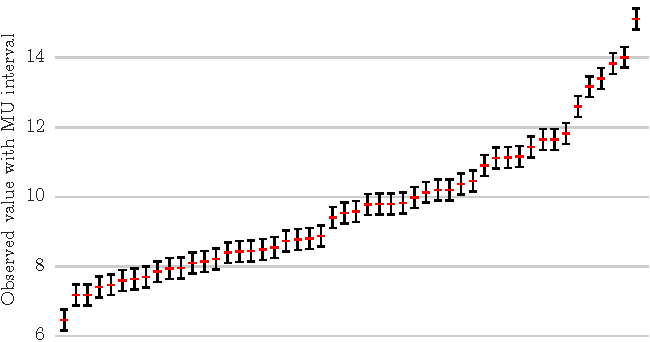
\includegraphics[]{obs_with_interval.pdf}
	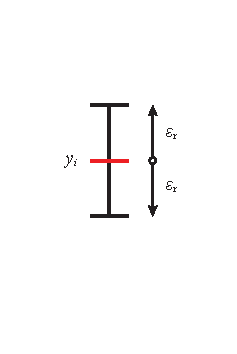
\includegraphics[]{MU_interval.pdf}
	\caption{Interval representation of measurement uncertainty (black) on a sorted random sample (red). The sample is generated from $Q_1$ with properties given in Table \ref{tab:prob_models_mu} and $CV_{Q_1} = 0.2$.}
	\label{fig:obs_with_interval}
\end{figure}

%*****************************************************************************************
\subsubsection{Statistical analysis}
An alternative approach to represent measurement uncertainty is statistical by means of probability distributions. The likelihood function depends on the reality-observation link (Eq.\ref{eq:ro_link}). This connection is also uncertain, but for simplicity, known relationship is assumed here and a possible treatment of this uncertainty is discussed in Section \ref{sec:discussion_mu}. Algebra of random variables can be used to obtain the likelihood function reflecting the distribution of involved random variables and the reality-observation link:
\begin{equation}
\label{eq:mu_like}
	L\left( {{{\boldsymbol{\theta }}_X},{{\boldsymbol{\theta }}_E}|{\mathbf{x}},{\boldsymbol{\epsilon }}} \right) = \prod\limits_{i = 1}^n {p\left( {h({x_i},{\epsilon _i})|{{\boldsymbol{\theta }}_X},{{\boldsymbol{\theta }}_E}} \right)}
\end{equation}
where ${\boldsymbol{\theta }}_X$ and ${\boldsymbol{\theta }}_E$ are the parameters of true and measurement uncertainty random variables, respectively.
In Approach~1, this means no additional complication because the observations are assumed to be distributed as the true random variable since the reality-observation link is neglected. However, in Approach~2b the likelihood function should be constructed to remove the effect of measurement uncertainty ($E$) from the variable of interest ($X$).
The \textit{measurement error problem} arises in many areas where only the contaminated values are attainable to the observer but the interest lays in the inference of true, uncontaminated values. Among others, these areas include astronomy, econometrics, biometrics, medical statistics, and image reconstruction \citep{Stefanski2000, Koen2009, Meister2009}. A straightforward solution is to construct the likelihood function (Eq.\ref{eq:mu_like}) and to infer the parameters of the variable of interest ($X$) by a selected method. To our knowledge this approach has not been applied in civil engineering yet.
Maximum likelihood method is used herein to infer the parameters in the statistical formulation of the measurement uncertainty problem.
Additive and multiplicative reality-observation links are considered. For the additive relationship: $Y = X + E$, the density function of the sum of two independent, continuous random variables is obtained by convolution:
\begin{equation}
\label{eq:conv}
	{f_Y}\left( y \right) = \left( {{f_X} * {f_E}} \right)\left( y \right) = \int\limits_{ - \infty }^\infty  {{f_X}\left( {y - x} \right)}  \cdot {f_E}\left( x \right) \cdot {\mathrm{d}}x.
\end{equation}
Here, for convenience the $p(.)$ notation of density functions is replaced with one that identifies the function elsewhere than in the argument, $f_X(x) \equiv p(x)$.
The integral can be efficiently solved by utilizing Fourier transformation since afterwards it reduces to a point-wise multiplication. Here, the fast-Fourier transformation is used to accomplish this task. For the multiplicative relationship: $Y = X \cdot E$, the density function of the product of two independent, continuous random variables is obtained by computing the following integral:
\begin{equation}
\label{eq:prod}
	{f_Y}\left( y \right) = \int\limits_{ - \infty }^\infty  {{f_X}\left( x \right)}  \cdot {f_E}\left( {\frac{y}{x}} \right) \cdot \frac{1}{{\left| x \right|}} \cdot {\mathrm{d}}x.
\end{equation}
This can be efficiently solved by Mellin transformation but here the integral is directly calculated due to the small computational burden.
Sampling variability (parameter estimation uncertainty) is accounted for by using the predictive reliability index, $\tilde \beta$ \citep{Kiureghian1989}:
\begin{equation}
\label{eq:predi_beta}
	 \tilde \beta  = \frac{{{{\mathrm{mean}}_B}}}{{\sqrt {1 + {{\mathrm{std}}_B}^2} }} \approx \frac{{{\mathrm{median}_B}}}{{\sqrt {1 + {{\left( {1.483 \cdot {{\mathrm{mad}}_B}} \right)}^2}} }}
\end{equation}
where $B$ is the posterior reliability index, std and mad are the standard deviation and median absolute deviation of $B$, respectively. The formulation with median and mad are used in this chapter, as that is more robust to outliers. Eq.\ref{eq:predi_beta} is an approximation as it is valid only for Normal distributed $B$. Additionally, the statistics are estimated from repeated analyses, and no Bayesian formulation of the reliability problem is used, even though that was used to derive the formula. For this study it is deemed sufficiently accurate to indicate tendencies and to identify critical cases.
\begin{figure}[htbp!] 
	\centering    
	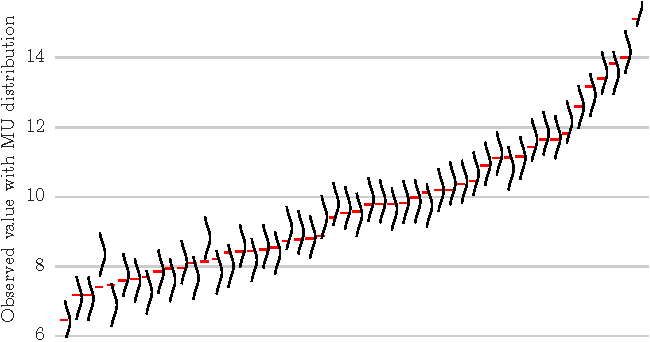
\includegraphics[]{obs_with_prob_error.pdf}
	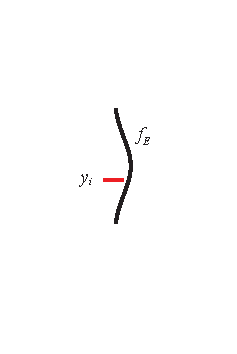
\includegraphics[]{MU_prob_distr.pdf}
	\caption{Illustration of probability distribution representation of measurement uncertainty (black) on a sorted random sample (red). The sample is generated from $Q_1$ with properties given in Table \ref{tab:prob_models_mu} and $CV_{Q_1} = 0.2$.}
	\label{fig:obs_with_prob_error}
\end{figure}

%****************************************************************************************
%****************************************************************************************
\section{Example: reliability of a generic structure}

%*****************************************************************************************
\subsection{Model description}
The reliability of a simple structural member is analyzed using a generic limit state function:
\begin{equation}
	 g = R - \left( {G + {Q_{50}}} \right).
	 %({\mathbf{X}})
\end{equation}

It represents a structure subjected to permanent ($G$) and variable ($Q_{50}$) actions, where the subscript 50 indicates 50-year reference period (common design working life). The probabilistic model of involved random variables are based on the recommendations of \citep{JCSS_basis} and summarized in Table \ref{tab:prob_models_mu}. For simplicity only the variable action is assumed to be affected by measurement uncertainty; it could be easily extended to more variables. Coefficient of variations 0.2, 0.4 for $Q_1$ represent annual snow maxima of mountains, highlands, while 0.6 characterizes lowlands in the Carpathian Region. The Lognormal model for snow maxima is typically adopted in the USA \citep{ASCE2010}, while the Gumbel model is widespread in Europe \citep{Sanpaolesi1998, JCSS_load}. The Normal and Gumbel distributions are light-tailed while the Lognormal is heavy-tailed. The adopted distributions and parameter ranges cover also other variable actions such as wind and thermal actions, thus the results can be readily generalized.

The annual maxima are assumed to be independent:
\begin{equation}
\label{eq:gfun_mu}
	{F_{50}}\left( q \right) = {F_1}{\left( q \right)^{50}}
\end{equation}
where $F(.)$ is the cumulative distribution function.

\begin{table}[htbp!]
\caption{Probabilistic models.}
\centering
\label{tab:prob_models_mu}
\small
	\begin{threeparttable}
    \begin{tabular}{llll}
    \toprule
    Variable name (symbol)  & Distribution & Mean & CV \\
    \midrule
    \rowcolor{lightgrey} Resistance ($R$)  & Lognormal & \tnote{*} & 0.10  \\
    Permanent action ($G$) & Normal &  8  & 0.10 \\
    \rowcolor{lightgrey} Variable action ($Q_1$)\tnote{\textdagger}  & Normal, Lognormal, Gumbel & 10 & $[0.20, 0.40, 0.60]$ \\
    \bottomrule
    \end{tabular}
    \begin{tablenotes}
    	\item[*] set to reach $\beta_\mathrm{target} = 3.8$ for each combination of inputs.
	    \item[\textdagger] the specified parameters are used to generate 50-element sample and the parameters of the model used in reliability analysis are inferred from it.  
   	\end{tablenotes}
   	\end{threeparttable}
\end{table}

\subsection{Interval and reliability analysis}
\label{subsec:interval_reli}
To model the effect of measurement uncertainty, 50 random observations are generated from $Q_1$, these are treated as observed ($Y$) values as the reality-observation link by definition is unknown in interval representation (Figure \ref{fig:int_alg}). Then intervals are centered at observations and various interval radiuses are considered. Using these interval variables, the distribution of $Q_1$ is fitted by the method of moments, which is a widely used approach in civil engineering \citep{Sanpaolesi1998} and was proved to be robust e.g. for modeling hydrological extremes \citep{Madsen1997}. The hybrid interval-probabilistic reliability problem is solved using optimization and first order reliability method (FORM). An outcome of the analysis is an interval reliability index.

The upper bound of it is irrelevant from safety point of view and the lower bound is recommended for practical applications \citep{Qiu2007}. This is due to the special nature of intervals and how they represent uncertainty: the real value can be anything within the interval but one cannot assume that all points are equally likely (principle of indifference) at least because the consequence of specific values are not equal. Hence we chose the recommended, careful engineering approach and use the lower endpoint of the reliability index interval as representative value.
\begin{figure}[htbp!] 
	\centering    
	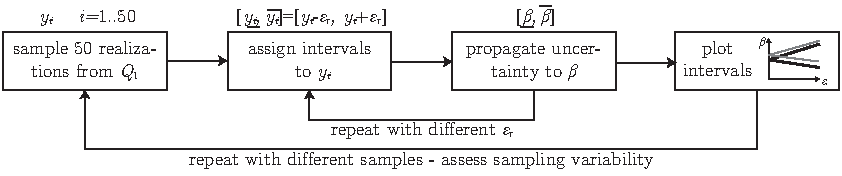
\includegraphics[]{interval_analysis_algorithm_.pdf}
	\caption{Algorithm of analyzing the effect of interval measurement uncertainty on reliability.}
	\label{fig:int_alg}
\end{figure}

\subsubsection{Full and approximate propagation of interval uncertainty}
As measurement uncertainty is expressed at the level of individual observations its full propagation yields to two distinct 50-dimensional constrained optimization problems that can be computationally demanding if each iteration step involves fitting a distribution function and solving a reliability problem. The computational burden can be considerably lessened by a two-step approximate technique where first the distribution parameters are fitted to the interval observations. Then only the interval representation of distribution parameters are used in further reliability analysis. Thus, the optimization with reliability analysis is reduced to a two-dimensional search space. Moreover, our experience show that the optimum is at the bounds so as it can be found by considering only the possible permutations of the parameter bounds.
The accuracy of full and two-step approximate uncertainty propagations are compared using Gumbel distributed $Q_1$. The results in terms of reliability indices are presented in Figure \ref{fig:beta_interval_full_approx}. The interval uncertainty is expressed as the ratio of interval radius and mean of annual maxima ($Q_1$). 0-10\% range is covered and it is assumed that all observations are contaminated with the same radius. For each coefficient of variation the mean of the resistance is set to reach the 3.8 target reliability level. This is performed by considering no measurement uncertainty ($\epsilon_\mathrm{r} = 0$) and using the parameters given in Table \ref{tab:prob_models_mu}, thus sampling variability has no effect. The calculated upper and lower reliability index endpoints are presented in the plots with solid and dashed lines for two-step and full propagations, respectively. Figure \ref{fig:beta_interval_full_approx} shows also the reliability index obtained by Approach~1. This is illustrated with a dotted line and is not affected by the assumed measurement uncertainty interval.
\begin{figure}[htbp!] 
	\centering    
	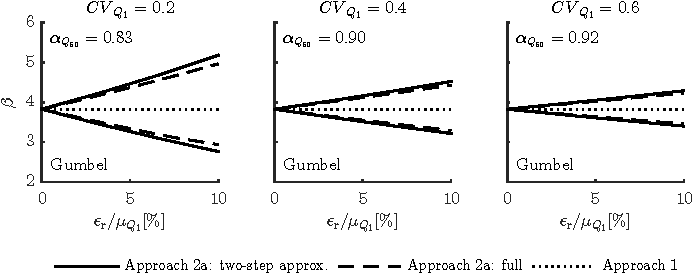
\includegraphics[]{beta_interval_full_approx.pdf}
	\caption{Reliability index intervals as the function of normalized measurement uncertainty radius ($\epsilon_\mathrm{r}/\mu_{Q_1}$) with full and approximate propagation of interval uncertainty.}
	\label{fig:beta_interval_full_approx}
\end{figure}

The plots show that the approximate technique slightly overestimates the accurate (full) reliability intervals, the largest difference is observed for $CV_{Q_1} = 0.2$ with large measurement uncertainty. Since in general the overestimation of the approximate technique is small, it is used in all further analysis. The sensitivity factor of the 50-year reference period maxima ($\alpha_{Q_{50}}$) is also displayed on the plots. It corresponds to a model without uncertainty in measurement and parameters. The decreasing interval range of $\beta$ with increasing $CV_\mathrm{Q1}$ is explained by the decreasing contribution of interval uncertainty to the full uncertainty of $Q_1$, i.e. aleatory uncertainty becomes dominating. Figure \ref{fig:explain_decr_beta_int} illustrates this shrinkage of uncertainty interval by comparing the transformed cumulative distribution functions with different coefficient of variations. The plots correspond to 50 particular random realizations; the same pattern is observed for other sets of random realizations.
\begin{figure}[htbp!] 
	\centering    
	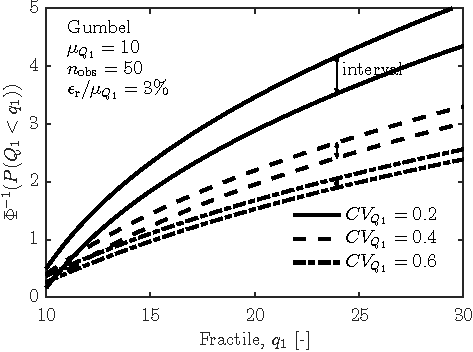
\includegraphics[]{explain_decr_beta_int.pdf}
	\caption{Illustration of the shrinkage of uncertainty interval with increasing coefficient of variation but constant measurement uncertainty interval.}
	\label{fig:explain_decr_beta_int}
\end{figure}

\subsubsection{Effect on reliability index and required resistance}
Eq.\ref{eq:gfun_mu} is solved for Normal, Lognormal and Gumbel distributed variable action ($Q_1$) using the two-step approximation technique. The results are summarized in Figure \ref{fig:beta_interval_small_multiples}; they have the same rationale as is given for Figure \ref{fig:beta_interval_full_approx}. The light gray lines show the opening reliability interval with increasing measurement uncertainty for 20 random samples, each with 50 realizations. These are indicative of the effect of sampling variability: in this case this is entirely parameter estimation uncertainty due to the finite sample size. The results show that sampling variability -- with 50 realizations, which is typical for maxima model of climatic actions -- has significant effect on reliability. It is dominating over measurement uncertainty for small interval radiuses and comparable for larger values. The thick black lines are the median of the 20 sample sets. The reliability index without considering measurement uncertainty can be seen at the common starting point of the lower and upper bound lines. The difference of this value and the lower bound is of interest here as it indicates the extent of the non-conservative neglect of measurement uncertainty. Based on our experience, the difference is deemed significant if it is larger than 0.5. This level is indicated by a dashed horizontal line while the significant range with a red half line. With the selected target reliability level, this corresponds to more than six-fold increase in failure probability.
\begin{figure}[htbp!] 
	\centering    
	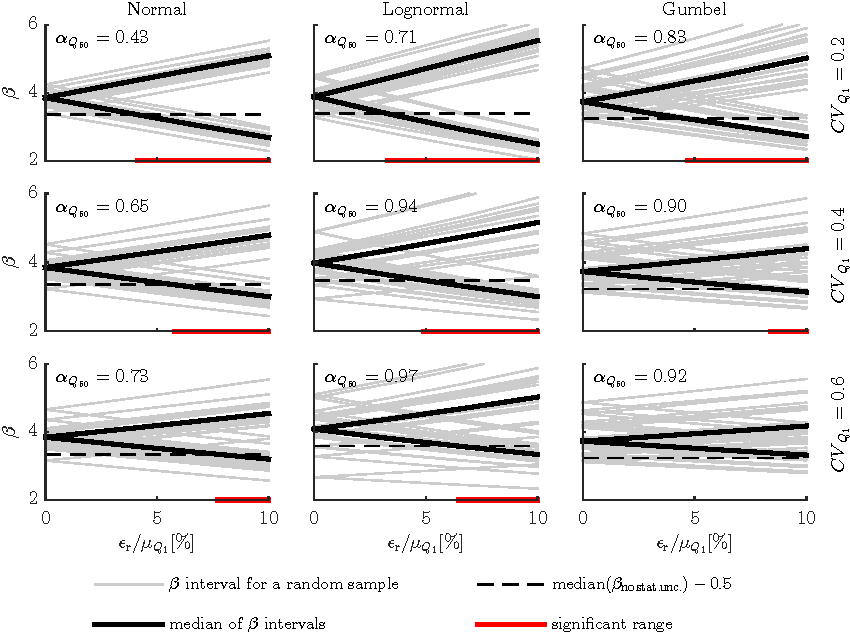
\includegraphics[]{beta_interval_small_multiples.pdf}
	\caption{Reliability index intervals as the function of the normalized measurement uncertainty radius ($\epsilon_\mathrm{r}/\mu_{Q_1}$). The gray lines represent 20 random samples, indicating sampling variability. The black lines are the median lower and upper interval endpoints of the reliability index. The red half line indicates the range where the lower endpoint of the reliability interval is significantly lower ($>0.5$) than the reliability calculated without measurement uncertainty ($\epsilon_\mathrm{r} = 0$).}
	\label{fig:beta_interval_small_multiples}
\end{figure}

The results suggest that moderate $\pm 4\%$ measurement uncertainty can lead to significant reduction of reliability level for mountains and highlands represented by $CV_{Q_1} = 0.2-0.4$. For the largest considered value of $CV_{Q_1} = 0.6$, the Gumbel model does not reach the limiting value. This indicates that for lowlands even a quite large $\pm 10\%$ measurement uncertainty has no practically significant effect. The reliability interval ranges indicate that even a small $\pm 2\%$ measurement uncertainty can lead to an order of magnitude uncertainty in the failure probability, see for instance the Lognormal distribution with $CV_{Q_1} = 0.2$. For larger measurement uncertainties, the width of the reliability intervals can be larger than 2.0; the widths are quite considerable for large $CV_{Q_1} = 0.6$ models too.
Measurement uncertainty thus seems to have a marked effect on structural reliability. The practical question then arises: what are its implications on design and how it should be accounted for? To examine this, we calculated the mean resistance ($\mu_R$) required to reach the target reliability with the lower bound of the reliability interval (Approach~2a). Then this value is compared to the $\mu_R$ required to reach the target reliability without explicit consideration of measurement uncertainty (Approach~1). The ratios of the mean values (with interval MU/without explicit MU) are illustrated in Figure \ref{fig:dspt_ratio_small_multiples}. These indicate how large adjustment might be needed in representative resistance values to meet target reliability in the presence of measurement uncertainty. The plots are structured and have the same rationale as Figure \ref{fig:beta_interval_small_multiples}. Based on our expertise, the ratio is deemed practically significant if it is larger than 1.1. This level is indicated by a dashed horizontal line while the significant range with a red half line. The small effect of sampling variability for Normal distribution is likely due to the small sensitivity factor of $Q_{50}$. On the contrary, sampling variability is quite considerable for Lognormal distribution. The selected threshold is reached for all distributions. The Lognormal model shows opposite trend, this might be attributed to its heavy tail. For this distribution the 1.1 threshold is reached at about 4\% normalized radius and the ratio can be over 1.4 for larger radiuses, which is a huge potential adjustment. The Gumbel distribution illustrates decreasing ratio with increasing coefficient of variation. For $CV_{Q_1} = 0.2$ (mountains), moderate $\pm 4\%$ measurement uncertainty can lead to significant $\mu_R$ ratio. For lowlands ($CV_{Q_1} = 0.6$), the ratio is over the selected threshold only for excessive measurement uncertainty $\pm 9\%$, which suggests that measurement uncertainty can be neglected for large values of $CV_{Q_1}$.
\begin{figure}[htbp!] 
	\centering    
	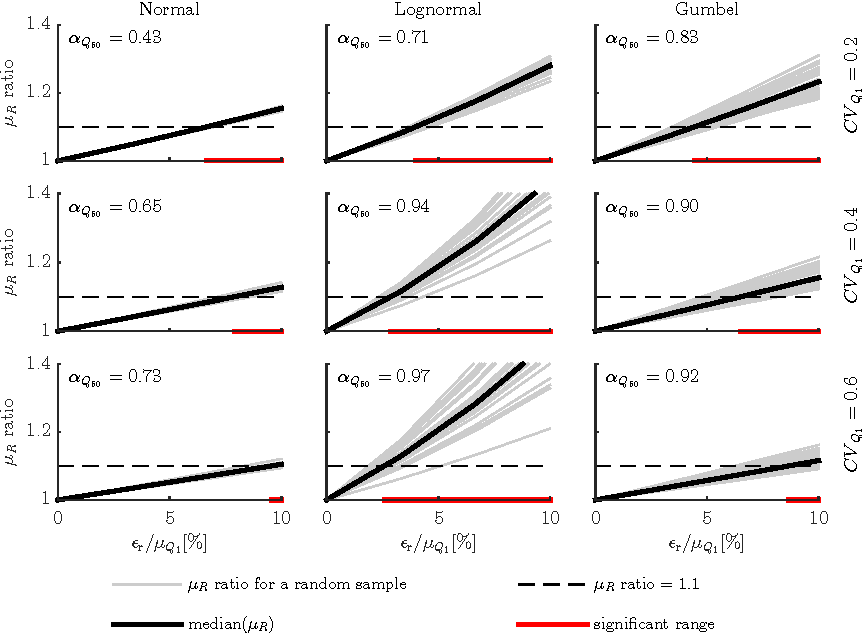
\includegraphics[]{dspt_ratio_small_multiples.pdf}
	\caption{Mean resistance ($\mu_R$) ratio for the variable action with and without measurement uncertainty as the function of the normalized measurement uncertainty radius ($\epsilon_\mathrm{r}/\mu_{Q_1}$). The red half line indicates the significant range where the ratio is larger than 1.1.}
	\label{fig:dspt_ratio_small_multiples}
\end{figure}

\subsection{Statistical and reliability analysis}
This section presents the statistical approach to quantify and propagate measurement uncertainty (Approach~2b). To model the effect of measurement uncertainty, 50 random observations are generated from $Q_1$ and treated as true ($X$) values. Then by using the assumed reality-observation link they are contaminated with measurement uncertainty. This is generated from a known, independent distribution ($E$). The algorithm is outlined in Figure \ref{fig:stat_alg}. Additive and multiplicative reality-observation links are assumed and the measurement uncertainty is taken as normally distributed with zero mean (unbiased). After the contamination of data, the information about the parameters of the underlying generating models -- with the exception of the zero mean of measurement uncertainty -- is disregarded and the maximum likelihood method is applied to decouple true values from measurement uncertainty. Finally, the model of decontaminated observations is used in reliability analysis. The sampling variability is again indicated by 20 samples and taken into account in an approximate manner through the predictive reliability index (Eq.\ref{eq:predi_beta}). The median and mean absolute deviation are calculated.
\begin{figure}[htbp!] 
	\centering    
	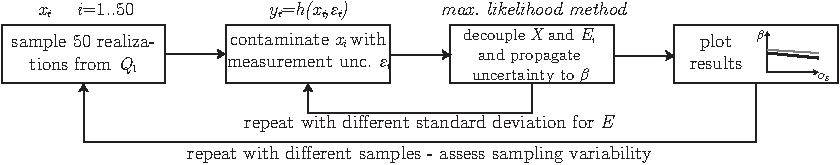
\includegraphics[]{statistical_analysis_algorithm_.pdf}
	\caption{Algorithm of analyzing the effect of measurement uncertainty on reliability using statistical technique.}
	\label{fig:stat_alg}
\end{figure}

\subsubsection{Decontamination of observations}
To illustrate the technique and the effect of decontamination, random realizations are generated from Gumbel distribution -- with parameters given in Table \ref{tab:prob_models_mu} -- and contaminated with measurement uncertainty (Figure \ref{fig:Gumbel_additive_me_smallm}). First, additive reality-observation relationship is assumed and Approach~1 and Approach~2b are used to infer the model parameters. The maximum likelihood method is used to obtain point estimates and the delta method is applied to construct $90\%$ confidence intervals to illustrate parameter estimation uncertainty \citep{Coles2001}.\mynote{ref to chapter 2!} The results for three cases of Gumbel distribution and two cases of measurement uncertainty with varying standard deviation are discussed only. The realizations and the fitted models are shown in Figure \ref{fig:Gumbel_additive_me_smallm}. It comprises return value-return period plots transformed to Gumbel space where the Gumbel distribution appears as a straight line. Though the plots are corresponding to a particular set of realizations, they convey reliably the trends and expected differences: (\textit{i}) Approach~1 typically overestimates the fractiles thus leading to lower reliability level and being conservative; (\textit{ii}) the difference between models increases with increasing return period. Due to the small sample size, the difference is affected by large sampling variability.
The calculations are repeated with multiplicative measurement uncertainty (Figure \ref{fig:Gumbel_prod_me_smallm}). The results correspond well with those obtained for the additive format. Furthermore, wider confidence intervals of Approach~2b compared with Approach~1 are observed. This is due to the larger model space where the same sample size allows less certain inference. This effect is less pronounced for the additive model.
For both models, Approach~1 is inherently biased since it is not using the correct likelihood function, while Approach~2b asymptotically converges to the true model. Thus, in the long run -- from theoretical point of view -- Approach~2b is better; however, Approach~1 seems to be generally conservative for the considered reality-observation links. This latter aspect is analyzed in more detail in the following section focusing on reliability index as a quantity of practical interest.
\begin{figure}[htbp!] 
	\centering    
	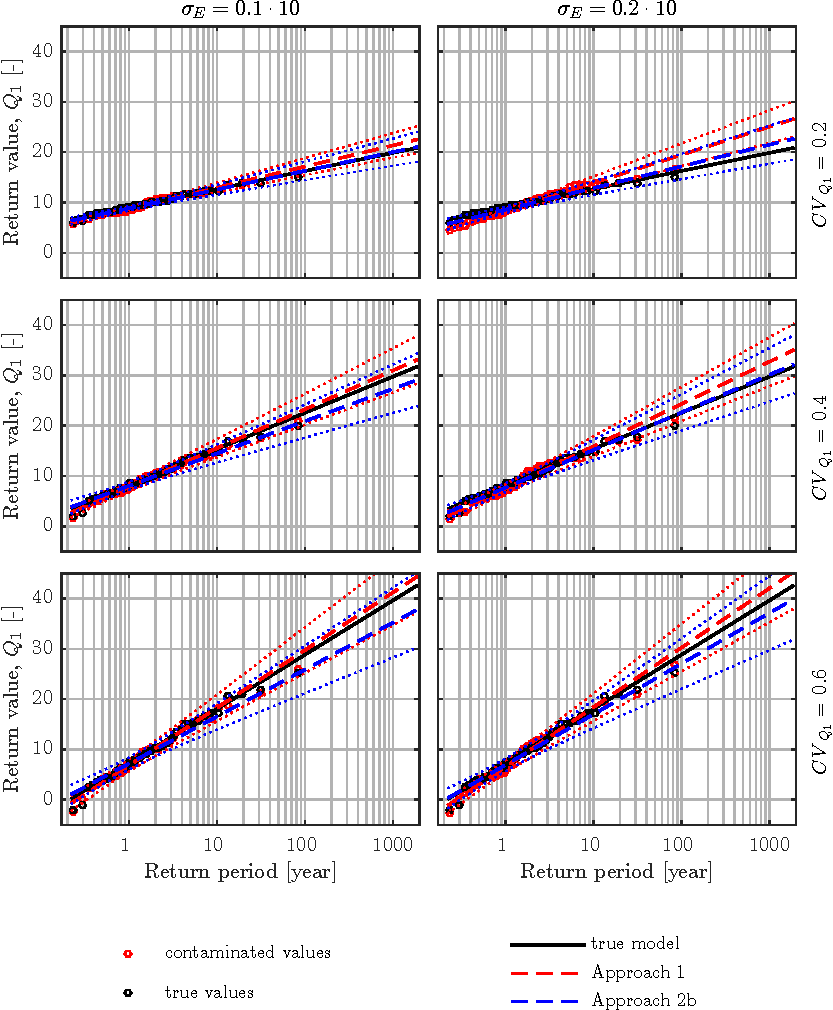
\includegraphics[]{Gumbel_additive_me_smallm_50_rng23.pdf}
	\caption{Gumbel distributions fitted to random realizations contaminated with additive measurement uncertainty using Approach~1 and Approach~2b. The point estimates (dashed lines) are accompanied by 90\% confidence intervals (dotted lines).}
	\label{fig:Gumbel_additive_me_smallm}
\end{figure}
\begin{figure}[htbp!] 
	\centering    
	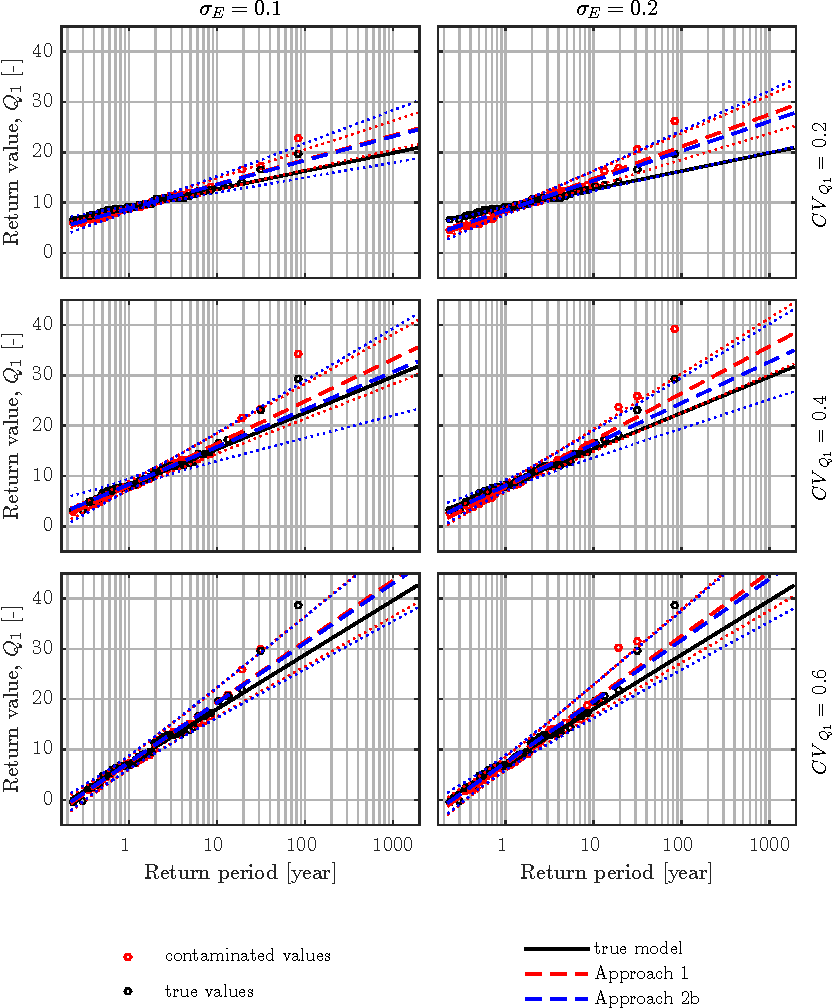
\includegraphics[]{Gumbel_prod_me_smallm_50_rng14.pdf}
	\caption{Gumbel distributions fitted to random realizations contaminated with multiplicative measurement uncertainty using Approach~1 and Approach~2b. The point estimates (dashed lines) are accompanied by 90\% confidence intervals (dotted lines).}
	\label{fig:Gumbel_prod_me_smallm}
\end{figure}

\subsubsection{Effect on reliability index}
The effect of measurement uncertainty on reliability index is analyzed for the additive relationship considering Normal, Lognormal and Gumbel distributed true values and with coefficient of variation ranging from 0.2 to 0.6. The measurement uncertainty has Normal distribution with known zero mean and varying standard deviation. Consistently with the interval analysis in Section \ref{subsec:interval_reli}, the mean value of the resistance is determined to reach the target reliability without measurement uncertainty and parameter estimation uncertainty. Then the algorithm presented in Figure \ref{fig:stat_alg} is applied to generate contaminated observations, to decontaminate them, and to calculate the reliability index using the inferred parameters. The calculations are repeated for 20 samples with sample size of 50. The results in terms of reliability indices are shown in Figure \ref{fig:Normal_lognormal_additive_me_beta_smallm} and in Figure \ref{fig:Gumbel_additive_me_beta_smallm}. Grey and light blue solid lines are representing the 20 samples, and the corresponding thick solid and dashed lines are the median and predictive reliability indices, respectively. The difference between these latter two lines expresses the effect of parameter estimation uncertainty. For Normal distribution, this effect is small compared to Lognormal and Gumbel for which it is increasing with increasing standard deviation of measurement uncertainty. For Approach~2b it is typically larger than Approach~1 as the larger model space allows less certain inference with the same sample size. In case of Lognormal and Gumbel models, the ratio of the predictive and median failure probabilities can be as large as an order of magnitude or larger. Additionally, the plots show that the reliability index can considerably be overestimated when parameter estimation uncertainty is neglected. The salient large scatter of Approach~2b might be partially attributed to the unstable maximum likelihood estimators for small samples \citep{Hosking1985, Martins2000}.
\begin{figure}[htbp!] 
	\centering    
	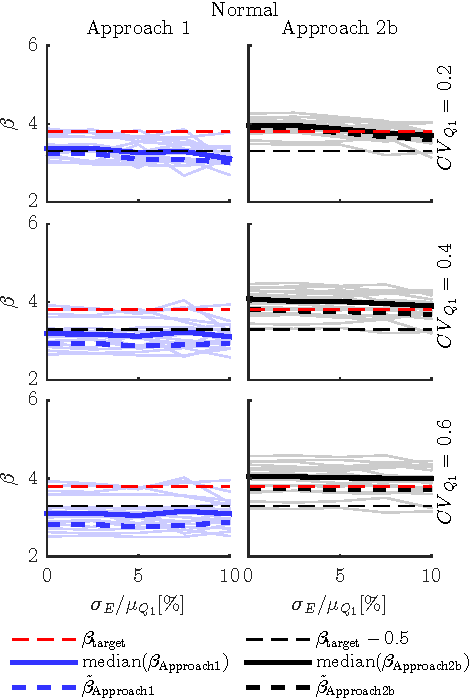
\includegraphics[]{Normal_additive_me_beta_smallm_666_median.pdf}
	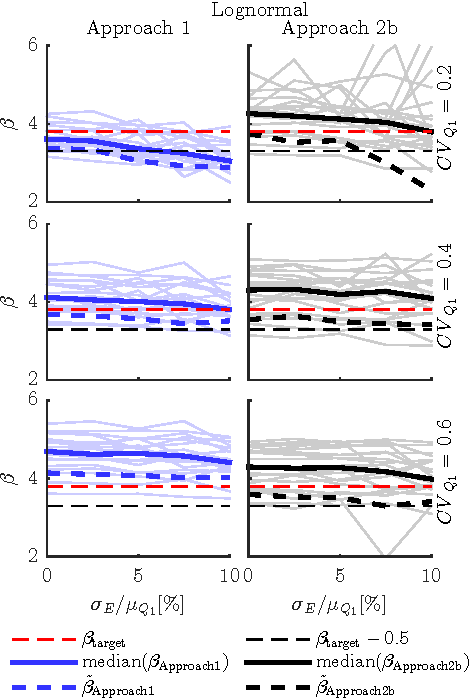
\includegraphics[]{Lognormal_additive_me_beta_smallm_666_median.pdf}
	\caption{Reliability indices as the function of the normalized standard deviation of measurement uncertainty ($\sigma_{E}/\mu_{Q_1}$). The thick solid lines are the median of the reliability indices while the thick dashed lines are the approximate predictive reliability indices.}
	\label{fig:Normal_lognormal_additive_me_beta_smallm}
\end{figure}

Comparing Approach~1 with Approach~2b for Normal and Gumbel distributions, the former approach yields to systematically lower reliability indices. The opposite trend observed for Lognormal distribution might be attributed to its heavy-tail. For Normal distribution, Approach~1 seems to be overly conservative, the median is well below the target reliability level. 
For all distributions, Approach~1 is reasonably conservative with the exception of Lognormal distribution and coefficient of variation of 0.6. However, even in this case the predictive reliability index corrects the overestimation. Though for Normal distribution it is too conservative, the currently prevalent Approach~1 appears to be safely applicable to measurement uncertainty problems in case of additive reality-observation relationship. Approach~2b is sound from theoretical point of view; however, its median overestimates reliability level, thus the predictive reliability index is to be used to avoid underestimation of failure probability. Its larger parameter estimation uncertainty can lead large reduction in reliability index for small sample sizes.
\begin{figure}[htbp!] 
	\centering    
	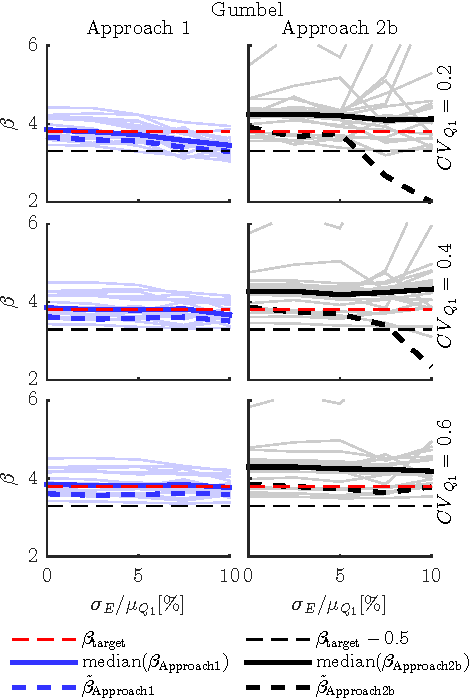
\includegraphics[]{Gumbel_additive_me_beta_smallm_666_median.pdf}
	\caption{Reliability indices as the function of the normalized standard deviation of measurement uncertainty ($\sigma_{E}/\mu_{Q_1}$). The thick solid lines are the median of the reliability indices while the thick dashed lines are the approximate predictive reliability indices.}
	\label{fig:Gumbel_additive_me_beta_smallm}
\end{figure}

%****************************************************************************************
%****************************************************************************************
\section{Application example: Turbine hall of Paks Nuclear Power Plant}
\label{sec:turbine_mu}

The turbine hall of Paks Nuclear Power Plant is selected to demonstrate the effect of measurement uncertainty on a real life example. The structure is introduced in Annex~\ref{sec:paks}, here only the essential details, which are required to interpret the results, are provided. The interval approach is used to represent measurement uncertainty and the two-step approximation is applied to propagate interval uncertainty. Annual ground snow maxima related to the location are contaminated with measurement uncertainty, the rest of random variables are represented by probability distributions. The results in terms of reliability indices and failure probabilities are given in Figure~\ref{fig:interval_beta_turbine_hall}. One year reference period is used for all calculations of the frame.

\begin{figure}[htbp!] 
	\centering    
	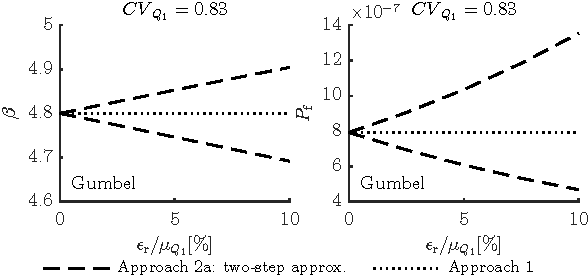
\includegraphics[]{interval_beta_turbine_hall.pdf}
	\caption{Reliability index and failure probability intervals as the function of normalized measurement uncertainty radius ($\epsilon_\mathrm{r}/\mu_{Q_1}$). Comparison of Approach~1 and Approach~2a for the turbine hall of Paks Nuclear Power Plant.}
	\label{fig:interval_beta_turbine_hall}
\end{figure}

The widest reliability index interval is 0.2, which is obtained for the largest measurement uncertainty error radius. This small value is in agreement with the trend observed in the previous example (Figure~\ref{fig:beta_interval_small_multiples}). It is attributed to the large coefficient of variation of annual ground snow load that is dominating over measurement uncertainty. In this example, neglect of measurement uncertainty leads to 70\% underestimation of failure probability at worst; hence, the effect is negligible.

%****************************************************************************************
%****************************************************************************************
\section{Discussion}
\label{sec:discussion_mu}
One can distinguish two components of measurement uncertainty: the reality-observation link and the nature of the contamination $E$. The three approaches considered here differ in how they treat these two components. The present prevalent approach (Approach~1) neglects both components, thus entirely ignores the possibility that the real values are greater or smaller than the observed due to measurement uncertainty.

The interval approach (Approach~2a) expresses full ignorance in respect of reality-observation link and represents measurement uncertainty with intervals. Therefore, no decoupling of true values from measurement uncertainty is possible. Intervals should be used with caution because by definition values outside of the interval are impossible. This assumption is rarely met in civil engineering. Measurement uncertainty is often described on the basis of expert judgment and wide intervals are applied to almost surely capture real, unobserved values.

The statistical approach (Approach~2b) requires the knowledge of the reality-observation link and represents measurement uncertainty with distribution function. This is the only approach that can decontaminate the observations and can directly infer the variable of interest, true variable. This is important since structural reliability is dependent on the true variable. The statistical and interval analysis based approaches are conceptually different, thus they are only comparable on that level but not quantitatively. Their uncertainty representation is inherently distinct, thus there is no equivalency between interval and distribution based representations.

Additionally, it must be emphasized that another type of uncertainty – statistical uncertainty in parameter estimation and selection of distribution function – often needs to be taken into account in reliability analysis as it may be even more important as measurement uncertainty investigated here \citep{RozsasIABSE2015, RozsasESREL2015}. Bayesian paradigm is a natural choice to incorporate this uncertainty, consequently that is recommended for practical applications. For example, in real-life situations, the reality-observation link cannot be established with certainty. Yet, this uncertainty can be captured by using multiple models and averaging them with respect their goodness of describing the data, this can be achieved for example by Bayesian model averaging \citep{Hoeting1999}.

Although this study is limited by the considered distribution types, reality-observation functions, and parameter range, it is believed to cover many practically relevant random variables. The presented approaches and algorithms can be easily used for other distribution types and measurement error structure. An additional limitation of this study is that measurement uncertainty is considered only for the dominant variable action. However, it is anticipated that for other random variables the effect is smaller due to their typically smaller sensitivity factor. Moreover, measurement uncertainty is much smaller for other than climatic actions such as resistance and permanent actions. Furthermore, the effect of sample size should be analyzed in later works. It is believed that the outcomes would be similar for sample sizes ranging from 20 to couple of hundreds, which cover the majority of cases in civil engineering. More data would allow more certain model identification.

%\section{Application example}

\section{Summary and conclusions}
The current practice in probabilistic engineering treats observed data contaminated with measurement uncertainty as realizations of the true distribution, thus neglecting the contamination mechanism. Statistical and interval-based analyses are thus conducted to investigate the effect of this simplification on structural reliability. Extensive parametric analyses -- based on 50 realizations, which is a typical length of records for climatic actions -- reveal that:\\
If interval representation of measurement uncertainty is used:
\begin{itemize}
	\item Sampling variability (parameter estimation uncertainty) has significant effect on reliability: it is dominant over measurement uncertainty for small interval radiuses and comparable for large radiuses.
	\item For mountains and highlands, moderate $\pm 4\%$ measurement uncertainty -- relative to value of an observed variable -- can lead to significant reduction of reliability level. For lowlands, even a large $\pm 10\%$ measurement uncertainty has no significant effect. An effect is deemed significant if it yields to greater than six fold increase in failure probability compared with Approach~1 (neglect of measurement uncertainty).
	\item Reliability interval ranges indicate that a small $\pm 2\%$ measurement uncertainty can lead to reduction of 0.6 in reliability index. For larger measurement uncertainties, the width of the reliability intervals can be larger than 2.0.
	\item The effect of measurement uncertainty is more pronounced for low variability random variables where its contribution to the total uncertainty increases.
	\item Parameter ranges where Approach~1 often overestimates the reliability index are identified.
\end{itemize}
If statistical (distribution function) representation of measurement uncertainty is used:
\begin{itemize}
	\item It is demonstrated that the statistical approach can be used to decontaminate the observations, thus to access the variable of interest.
	\item The ratio of the predictive and median failure probabilities can be as large as an order of magnitude or larger ($\sim30$ for Lognormal distribution).
	\item If parameter estimation uncertainty is disregarded, the reliability index can be considerably overestimated.
	\item For all considered distributions with additive measurement uncertainty, Approach~1 is reasonably conservative in most cases.
\end{itemize}

Practical recommendations:
\begin{itemize}
	\item Figure \ref{fig:beta_interval_small_multiples} and Figure \ref{fig:dspt_ratio_small_multiples} can be used to identify cases when Approach~1 significantly overestimates reliability index. In such cases and when no or very limited information on measurement uncertainty is available, then interval analysis could be used, considering the lower bound of the reliability interval.
	\item If the reality-observation link is known then the statistical approach is recommended. For small and moderate sample sizes ($<100$), the predictive reliability index is recommended. For additive measurement uncertainty, Approach~1 is conservative.
	\item For point estimates, such as median, the reliability index should be accompanied by uncertainty intervals to indicate the credibility of results.
	\item For ground snow extremes at lowlands, Approach~1 provides a reasonable approximation, thus the effect of measurement uncertainty can be neglected. Otherwise more advanced analysis is recommended.
\end{itemize}

Assessment of measurement uncertainty should be region- and case-specific accounting for measuring techniques, and applied correction equations, thus involvement of meteorologists, analysts or other experts is beneficial. Moreover, the selected approach to propagate measurement uncertainty should always be based on the particular issue in question, acknowledging ``the degree of precision to which the nature of the subject admits''.
\chapter{Long-term trends in annual ground snow maxima}
\label{cha:time_trend}

% **************************** Define Graphics Path **************************
\ifpdf
    \graphicspath{{Chapter5/Figs/Raster/}{Chapter5/Figs/PDF/}{Chapter5/Figs/}}
\else
    \graphicspath{{Chapter5/Figs/Vector/}{Chapter5/Figs/}}
\fi

% **************************** Chapter Abstract ******************************
\leftskip=1cm
\noindent
\emph{The current structural design provisions are prevalently based on experience and on the assumption of stationary meteorological conditions. However, the observations of past decades and advanced climate models show that this assumption is debatable. Therefore, this chapter examines the historical long-term trends in ground snow load maxima and their effect on structural reliability. Annual maxima snow water equivalents are taken and univariate generalized extreme value distribution is adopted as a probabilistic model. Stationary and five non-stationary distributions are fitted to the observations utilizing the maximum likelihood method. Statistical and information theory based approaches are used to compare the models and to identify trends. Finally, reliability analyses are performed on a simple structure to explore the practical significance of the trends. The calculations show decreasing trends in annual maxima for most of the region. Although statistically significant changes are detected at many locations, the practical significance -- with respect to structural reliability -- is considerable only for a few, and the effect is favorable. The results indicate that contrary to the widespread practice in extreme event modeling, the exclusive use of statistical techniques on the analyzed extremes is insufficient to identify practically significant trends. This should be demonstrated using practically relevant examples, such as reliability of structures.}

\leftskip=0pt\rightskip=0pt

\mynote{it would be interesting to make a simple analysis regarding duration of snow covar, number of days with snow cover, maybe an annex}

%****************************************************************************************
%****************************************************************************************
\section{Problem statement and the state of the art}

The provisions of current structural standards are based on the assumption that the underlying natural phenomena -- generating the actions on structures, and determining their working environment -- are stationary. However, observations of the past decades and advanced meteorological analyses show that this assumption does not represent accurately the present, either the future world \citep{IPCC2012extremes, Milly2008, Herring2015}. Hence, the aim of this chapter is to analyze the long-term trends in snow events and their implications on structural reliability. The Carpathian Region is selected for the study and the database presented in Section \ref{sec:data_under_study} is used.

Previous studies indicate that there is a statistically significant time-trend in snow events for the region. \citet{Birsan2014} have analyzed historical observations from Romania and detected decrease in snowfall days (82\% of stations) with substantial decrease in snow depth (18\% of stations) and also in snow coverage (29\% of stations). 

\mynote{\citet{Pecho2009} found statistically significant decrease(increase?, poor quality study, should be included?) in five-day total precipitation and fresh snow cover depth for Slovakia.} 

To our knowledge the long-term trends in extreme snow loads, e.g. annual maxima, for the Carpathian Region have not been sufficiently analyzed yet. Moreover, we are not aware of any study quantitatively analyzing the effect of time-trends in snow loads on structural reliability.  Although \citet{Pecho2009} and \citet{Sadovsky2007} examined time-trends in snow precipitation for the Slovakian Alps, their study is insufficiently documented, which  makes it difficult to evaluate the merit and value of their work. From the available information it appears that their approach  is not able to answer the main questions of this chapter.
%, e.g. statistical significant changes are claimed; however, neither the applied test nor the significance level are documented. A similar study by  of the same region is better documented but besides the limited scope of the study it contains conceptual errors, e.g. it is undocumented how the authors used the Kolmogorov-Smirnov test (null and alternative hypotheses) although even without these details its use is incorrect since that requires completely specified distribution function to be compared with observations \citep{Lilliefors1967}. This criterion is certainly not met in the study, thus the use of Kolmogorov-Smirnov test is erroneous. Moreover, the authors base their conclusions on the outcome that all tests are passed. This is a misinterpretation of statistical null hypothesis tests. Note that even if the tests were conducted correctly, the conclusions should have been supported by additional analysis due to the limitations of null hypothesis significance testing \citep{Carver1993, Wagenmakers2008}.

An excellent study is available for the Swiss Alps where \citet{Marty2012} detected statistically significant negative, long-term trends in annual snow depth. However, their analysis is focused on statistical significance testing and on return values. Thus, although indicating interesting tendencies, the practical significance of their results, e.g. with respect to structural reliability cannot be judged. This is partially inevitable since practical significance differs by end-users. Therefore, in this chapter a more pragmatic approach is promoted in which after the statistical analysis the practical significance of the findings is examined. The main interest here is the impact of snow trends on structural reliability, particularly on the probability of structural failure. Only historical observations are considered but a worthwhile extension would be to incorporate the projections of global climate models. In a recent study \citet{Ogorman2014} showed that no considerable change is expected in the 20-year return period extreme snow events for the North American region up to the end of the 21st century, though the impact on structural reliability is inconclusive since that is governed by rarer events.

%****************************************************************************************
%****************************************************************************************
\section{Solution strategy}

Univariate generalized extreme value (GEV) distribution is selected as it is widely accepted in extreme value analysis \citep{Klein2009} and was successfully applied for modelling extreme precipitations \citep{Coles2003catastrophes}, temperatures \citep{Guttorp2011}\mynote{one ref is missing, ot Eriksson2013}, discharges \citep{Hao2015}, wind speeds \citep{Hundecha2008} and waves \citep{Caires2006}. Stationary and non-stationary models are compared based on how likely the data are generated by each model. The considered non-stationary distributions with time-dependent parameters are summarized in Table \ref{tab:nonstat_dist}. The shape parameter is constant in all presented models, this is explained by that models with shape parameter linearly varying in time yielded to considerably worse fit than the others and often lead to unrealistic fractiles. The adopted block length is one year, covering a whole winter season. Furthermore, to account for seasons without snow the cumulative distribution function of annual maxima is expressed as follows:
\begin{equation}
	P\left( {X < x} \right) = P\left( {{\mathrm{snowfall}}} \right) \cdot P\left( {X < x|{\mathrm{snowfall}}} \right)
\end{equation}
where the former event has Bernoulli, while the latter has GEV distribution.

Maximum likelihood method is selected for parameter estimation due to the large number of locations. According to \citet{Hosking1985} and \citet{Martins2000} the maximum likelihood method can lead to unstable parameter estimation for small sample size; however, it is deemed to be sufficient for this exploratory analysis. Bayesian approach might be used to overcome the issue of instability for further detailed studies.
\mynote{The method of moments is not suitable to handle non-stationary models, since the aggregated statistics (moments) do not contain information about the order of the observations, which is crucial to capture time-dependency (Section \ref{subsec:point estiamtes}).}

\begin{table}[htbp!]
\caption{Summary of the considered non-stationary GEV distributions.}
\centering
\label{tab:nonstat_dist}
\small
    \begin{tabular}{llll}
    \toprule
    Model ID  & Location par. ($\mu$) & Scale par. ($\sigma$) & Shape par. ($\xi$) \\ 
    \midrule
    \rowcolor{lightgrey} $\mu 1$  & $a_0 + a_1 \cdot t$  & constant  & constant \\
    $\mu 2$  & $b_0 + b_1 \cdot t+ b_2 \cdot t^2$  & constant   & constant \\
    \rowcolor{lightgrey} $\sigma 1$  & constant  & $d_0 + d_1 \cdot t$  & constant \\
    $\sigma 2$  & constant  & $e_0 + e_1 \cdot t+ e_2 \cdot t^2$  & constant \\
    \rowcolor{lightgrey} $\mu 1\sigma 1$ & $g_0 + g_1 \cdot t$  & $g_2 + g_3 \cdot t$ & constant   \\ 
    \bottomrule
    \end{tabular}
\end{table}

Likelihood ratio (LR) test and Akaike information criterion (AIC) are used to compare the stationary and non-stationary models. The former is a standard frequentist hypothesis test for comparing nested models \citep{Wilks1938}. The latter is an asymptotic information criterion that is based on the premise that the model with smallest information loss (Kullback-Leibler divergence) should be preferred \citep{Wit2012}. In the absence of the true model, the information loss cannot be calculated in absolute terms; however, the models can be compared and their relative ``strength'' can be expressed by the difference in AICs or by using Akaike weights (Eq.\ref{eq:Akaike_weight}). Herein the corrected form of Akaike information criterion (AICc, Eq.\ref{eq:AICc}) is applied that takes into account the effect of a finite sample size. The goodness-of-fit of the models is visually checked using Q–Q, P–P, and return-period–-return value plots \citep{Coles2001}. These plot types are defined in Annex~\ref{sec:prob_plots}. Additionally, at some locations the GEV model is compared to other commonly applied distributions for diagnostic purposes, i.e. Gumbel and three-parameter Lognormal. Due to the limitations of statistical significance testing \citep{Carver1993} the effect size, power of the test, and confidence intervals are also utilized to compare the models. The conclusions are based on the practical bearing of these models on structural reliability.

%****************************************************************************************
%****************************************************************************************
%\section{Results and discussion}

%****************************************************************************************
%\subsection{Historical observations 1962-2011}

%****************************************************************************************
%****************************************************************************************
\section{Stationary model}
Stationary GEV distribution is fitted to each of the 5895 grid points using the ML method; the corresponding shape parameters are plotted in Figure~\ref{fig:shape_map}. This map and all the others in the following are created using equidistant conic projection and linear interpolation. In Figure~\ref{fig:shape_map}, the areas bounded by black contours indicate Weibull distribution, it can be seen that the high mountainous areas have dominantly this upper bounded distribution type. Considerable part of the studied area has Fréchet distribution with relatively large shape parameter ($\xi > 0.2$), which is in conflict with the Gumbel assumption widely accepted in Europe \citep{Sanpaolesi1998}, EN 1991-1-3:2003 and ISO 4355:2013. Additional limitation of the Gumbel distribution is that it yields to artificially narrower confidence intervals than the Fréchet as its parameters span smaller space, see Chapter \ref{cha:stat_unc} and \citet{Coles2003catastrophes}.

\begin{figure}[htbp!]
	\centering    
	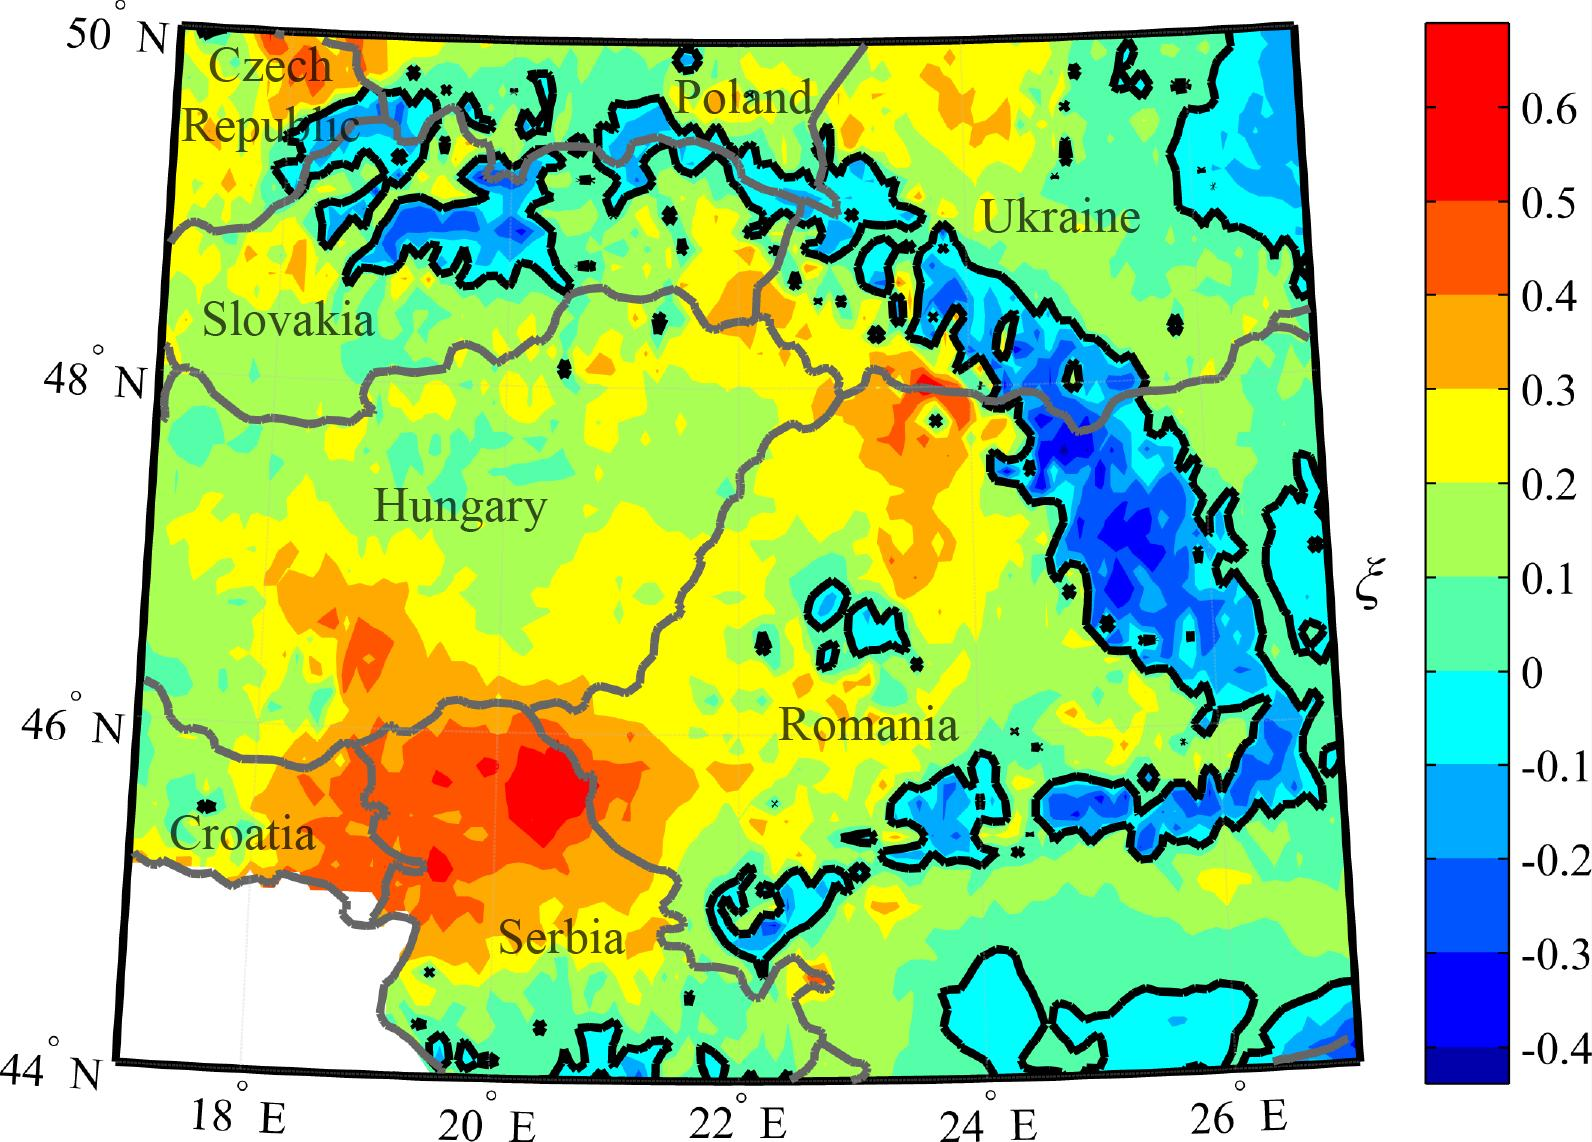
\includegraphics[width=0.5\textwidth]{stat_shape_parameter_map_crude_names.jpg}
	\caption{Shape parameter ($\xi$) of the fitted, stationary GEV distributions, the black contour surrounds the Weibull type.}
	\label{fig:shape_map}
\end{figure}

The unfavorable deviation from Gumbel distribution is the most pronounced in the northern part of Serbia. It is interesting that some locations exhibit shape parameter larger than 0.5, which means that the distribution has infinite variance. If this is deemed to be unrealistic, it might be avoided by adopting constraints in ML or by using Bayesian approaches with appropriate priors.

%****************************************************************************************
%****************************************************************************************
\section{Long-term trends, non-stationary models}
First, a straight line is fitted to the annual maxima (Figure~\ref{fig:trend_line}) at every grid point in the least-squares sense, while the snow-free years are discarded from the analysis. The associated slope parameters are illustrated in Figure~\ref{fig:trend_map}, where the negative values are referring to decreasing trends in time. At 97\% of the locations decreasing trend is identified, whereas a mild increase is observed in the northern part of the region -- Slovakia, the Czech Republic, and Poland. The small regions with strong, increasing trends next to decreasing ones (orange areas surrounded by dark blue ones) in Slovakia and Ukraine imply discrepancy in the database. Areas with the most pronounced decreasing trend are matching well with the Weibull regions with the exception of the southern part. Based on the linear trend the average change in annual maxima for the entire region during observation period is -42\%, compared to the 1962 level.

\begin{figure}[htbp!]
	\begin{subfigure}[b]{0.43\textwidth}    
		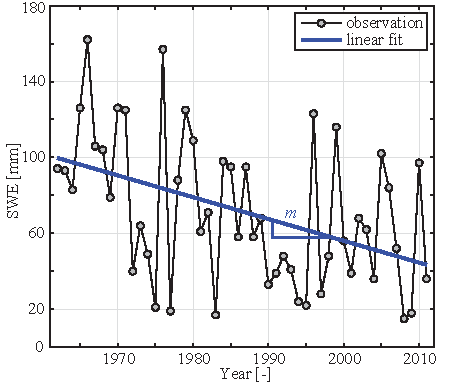
\includegraphics[width=\textwidth]{sample_time_trend.pdf}
		\caption{A representative location with decreasing trend.}
		\label{fig:trend_line}
	\end{subfigure}
	\hfill
	\begin{subfigure}[b]{0.52\textwidth}
		\includegraphics[width=\textwidth]{amax_timetrend_linreg_slope_paper.jpg}
		\caption{Map of the linear trend line’s slope parameter $m$ in mm/year.}
		\label{fig:trend_map}
	\end{subfigure}
	\caption{Fitting linear line to the annual maxima ground snow loads.}
\end{figure}

A more involved, LR and Akaike weight based comparisons of the stationary and five non-stationary GEV distributions show that the models with time-variant location parameters fit better the observations than those with time-variant scale parameter. Comparison between the models with time-variant location parameter reveals that the $\mu 1$ model performs the best for most of the area. The LR and Akaike weight based results, comparing the $\mu 1$ and stationary models are presented in Figure~\ref{fig:LR_mu1} and \ref{fig:AW_mu1}. Albeit both figures are showing probabilities ($P$), their interpretation is substantially different. In case of the LR test it expresses the probability that if the null hypothesis is true (stationary model) the difference between the log-likelihoods is at least as large as the one observed. This probability is typically referred as the $p$-value, and Figure~\ref{fig:LR_mu1} is showing the complementer of it ($P = 1 - p$). On the other hand, the Akaike weights –- illustrated in Figure~\ref{fig:AW_mu1} -– express the probability that $\mu 1$ model is better than the stationary one in the Kullback-Leibler divergence sense. In respect of these probabilities, the selected threshold is 90\% in both cases. Locations above this value are marked with a dot and considered as statistically significant. The vast majority of the statistically significant trends identified by the LR test are decreasing (black dots), only two locations in the Czech Republic show significant increase (white dots in the upper left corner in Figure~\ref{fig:LR_mu1}). The Akaike weight based comparison shows solely decreasing trends. The LR test is identified much more locations with significant trend, although the probabilities are not directly comparable. In addition, 65\% of these locations are statistically significant even with 95\% threshold level as well. The trends might be explained by the diminishing number of snow days as a consequence of increasing mean global temperature.

\begin{figure}[htbp!]
	\begin{subfigure}[b]{0.49\textwidth}    
		\includegraphics[width=\textwidth]{LR_test_stat_m1_p0_90_crude.jpg}
		\caption{Likelihood ratio.}
		\label{fig:LR_mu1}
	\end{subfigure}
	\hfill
	\begin{subfigure}[b]{0.49\textwidth}
		\includegraphics[width=\textwidth]{A_weight_stat_m1_p0_90_crude.jpg}
		\caption{Akaike weight.}
		\label{fig:AW_mu1}
	\end{subfigure}
	\caption{Comparison of $\mu 1$ and stationary models, grid-points with $P > 0.90$ are marked with dots: black for decreasing and white for increasing trends.}
\end{figure}

A more pragmatic comparison of time-trends is presented in Figure~\ref{fig:char_nonstat}, where the 50-year return values for stationary and non-stationary $\mu 1$ models are compared. The 50-year return value is referred as characteristic value in structural engineering and serves as the basis of everyday design. All the selected locations, shown in Figure~\ref{fig:char_nonstat}, exhibit significant negative trend in AICc sense.

\begin{figure}[htbp!]
	\centering
	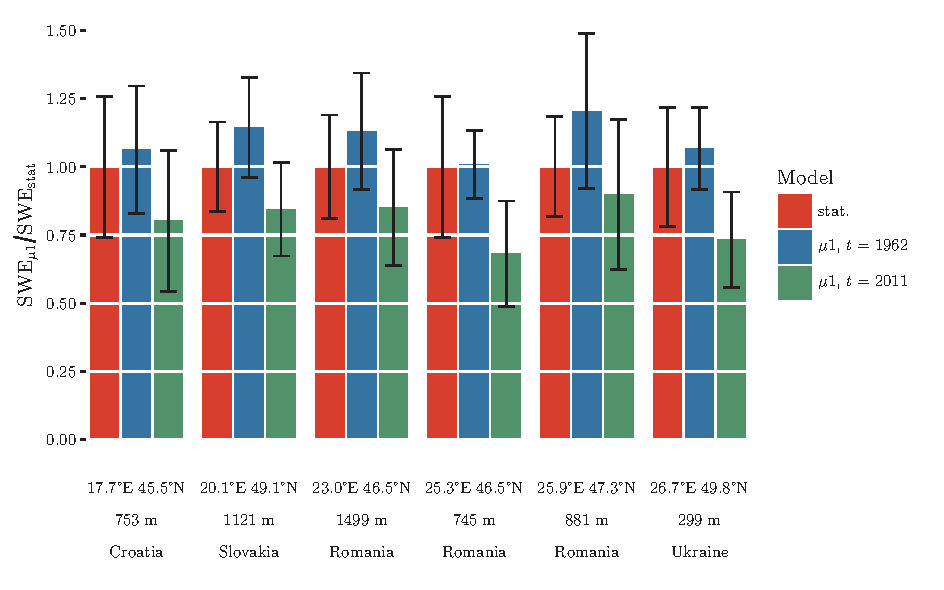
\includegraphics[width=1\textwidth]{char_values_stat_nonstat.pdf}
	\caption[]{Normalized 50-year return value SWE with 90\% confidence intervals (black) for selected locations that have significant negative trends as identified by Akaike weights \mynote{\footnotemark}.}
	\label{fig:char_nonstat}
\end{figure}
%\footnotetext{The countries are identified by ISO 3166-1 Alpha-3 codes.}

Figure~\ref{fig:char_nonstat} also shows that even for the locations where the AICc based criterion identified significant trends, in respect of 50-year return value with 90\% confidence interval, the difference is not always practically significant. The time-trend is deemed practically significant if the stationary estimate is outside of the non-stationary confidence interval. For the entire region, the average change characteristic values between 1962 and 2011 is $-10\%$, using the $\mu 1$ model and 1962 as reference. For locations with statistically significant trends the changes are $-19\%$ and $-26\%$ for LR test and Akaike weights respectively.

%****************************************************************************************
%****************************************************************************************
\section{Impact on structural reliability}

Although the focus of this chapter is the statistical characterization of snow loads and identification of trends in annual maxima, the key question from an engineering point \mynote{do not break here!!} of view is the effect of the changes on structural reliability and the adequacy of current provisions. The simple statistical, information theory (LR, AICc), and representative fractile based comparisons cannot answer this question, since the failure probability of a structure is dominantly determined by the tail of the distribution functions, well above or below the characteristic value. Thus, a simple, illustrative example is selected to explore this question. The related limit state function and the properties of the random variables are given in Eq.~\ref{eq:time_trend_gfun} and in Table~\ref{tab:time_trend_probmod}, respectively. For simplicity, the distribution functions of annual snow maxima are used and annual failure probabilities are calculated. Exceptional snow loads and accidental load combinations are not covered in the analysis.
\begin{equation}
\label{eq:time_trend_gfun}
	g(\mathbf{X}) = R - \left( {G + \mu  \cdot S } \right)
\end{equation}


\begin{table}[htbp!]
\caption{Summary of the considered non-stationary distributions.}
\centering
\label{tab:time_trend_probmod}
\small
	\begin{threeparttable}
    \begin{tabular}{lllll}
    \toprule
    Variable  & Distribution & Mean & CV & Reference \\
    \midrule
    \rowcolor{lightgrey} Resistance, $R$  & Lognormal & 1000/350\tnote{*} & 0.12  & \cite{JCSS_resi}  \\
    Ground snow, $S$ & GEV & \tnote{\textdagger} & \tnote{\textdagger}  & --  \\
    \rowcolor{lightgrey} Ground to roof conversion factor, $\mu$  & Lognormal & 0.75 & 0.15  & \cite{JCSS_load}  \\
    Permanent action, $G$  & Normal & 50 & 0.10  & \cite{JCSS_load}  \\
    \bottomrule
    \end{tabular}
    \begin{tablenotes}
    	\item[*] 1000 for the Hungarian, and 350 for the Ukrainian locations to achieve realistic and comparable reliability level.
	    \item[\textdagger] varies according to the selected model.  
   	\end{tablenotes}
   	\end{threeparttable}
\end{table}

Reliability analyses are performed for two representative locations using standard, first order reliability analysis (FORM). The first one is the Ukrainian location presented in Figure~\ref{fig:char_nonstat}. It has small, scattered settlements and it represents the significant negative trend even in respect of 50-year return values. The second is the fifth most populous city in Hungary (Pécs), it is identified by the LR test with statistically significant negative trend. It represents the moderate negative trend, which reflects well the majority of the region. These two locations are referred hereinafter as Ukrainian and Hungarian. Reliability is analyzed considering a reference period of one year. The location parameter is obtained from the non-stationary model for each of the selected years: 1962, 2011 and 2062. The delta method is used to construct approximate confidence intervals for these indices, and the results are summarized in Figure~\ref{fig:beta_nonstat}.

\begin{figure}[htbp!]
	\centering
	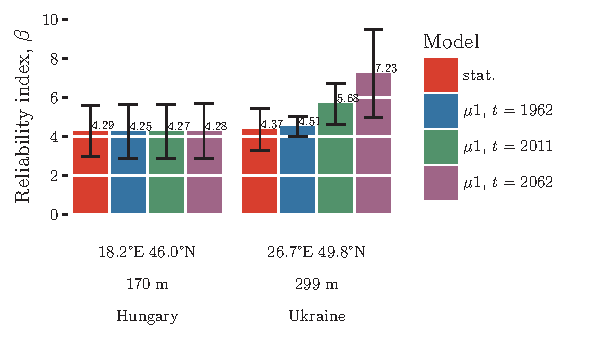
\includegraphics[width=0.7\textwidth]{beta_values_stat_nonstat.pdf}
	\caption{Reliability indices with 75\% confidence intervals (black) from ground snow parameter estimation uncertainty.}
	\label{fig:beta_nonstat}
\end{figure}

From Figure~\ref{fig:beta_nonstat} it is clear that the moderate decreasing trend has almost no effect on structural reliability, it is dwarfed by the parameter estimation uncertainty. For the Ukrainian location the increase in reliability level is practically significant, although the uncertainty is large here as well. From safety point of view, the change is clearly favorable, and whether the current provisions will provide economical design for these locations in the future is a different issue. The most important factor in the difference of the results for the Hungarian and Ukrainian locations is that the former has Fréchet while the latter has Weibull distribution.
The extrapolation of the non-stationary model to 2062 should be handled with care, it is provided only for illustrative purposes. It introduces additional uncertainty for non-stationary models as illustrated for the Ukrainian location in Figure~\ref{fig:extrap_nonstat}. This should be reduced by use of physical models or further explanations. 

\begin{figure}[htbp!]
	\centering
	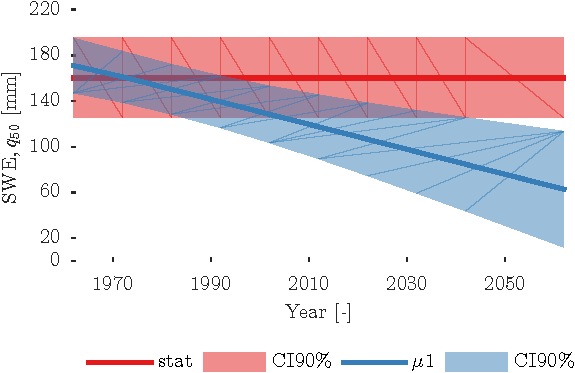
\includegraphics[width=0.7\textwidth]{stat_nonstat_conf_int_time_02.pdf}
	\caption{Ukrainian location, 50-year return value SWE ($q_{50}$) with 90\% confidence bands (CI90\%) for stationary (stat) and $\mu 1$ models.}
	\label{fig:extrap_nonstat}
\end{figure}

%***************************************************************************************
\subsection{Application example: Turbine hall of Paks Nucelar Power Plant}
\label{sec:turbine_trend}

Non-stationary extreme value analyses of annual ground snow maxima are conducted for the site of the turbine hall of Paks Nuclear Power Plant. The structure is introduced in Annex~\ref{sec:paks}, here only the essential details, which are required to interpret the results, are provided. Table~\ref{tab:nonstat_fit_paks} summarizes the Akaike weights and some representative fractiles for the selected models; the parameters are estimated using maximum likelihood method. The Akaike weights favor the stationary model, while the second best model is the one with linearly varying location parameter ($\mu1$). The fractiles of non-stationary models show small decrease in time.

The stationary and $\mu1$ models are used to calculate the annual reliability index of the structure in three distinct years (1962, 2011, and 2062). Furthermore, the parameter estimation uncertainty of ground snow load model is propagated to reliability index by using the delta method. The results are presented in Table~\ref{tab:nonstat_beta_paks}, from which it is salient that parameter estimation uncertainty dominates over the time-trend caused change in reliability index.

\begin{table}[htbp!]
\caption{Akaike weights and representative fractiles of the fitted stationary and non-stationary GEV distributions for the site of Paks Nuclear Power Plant. Fractiles are given for the years of 1962 and 2011.}
\centering
\label{tab:nonstat_fit_paks}
\small
	\begin{threeparttable}
	    \begin{tabular}{llllll}
	    \toprule
	    \multirow{2}{*}{Model ID} & \multirow{2}{*}{$w$\tnote{*}} & \multicolumn{2}{l}{$q_{50}$ [kN/m$^2$]} & \multicolumn{2}{l}{$q_{1000}$ [kN/m$^2$]} \\
	     &  & 1962  & 2011 & 1962 & 2011 \\ 
	    \midrule
	    \rowcolor{lightgrey} stat.       & 0.439 & 1.53 & 1.53 & 4.83 & 4.83 \\
	    $\mu 1$                          & 0.190 & 1.55 & 1.49 & 4.82 & 4.76 \\
	    \rowcolor{lightgrey} $\mu 2$     & 0.092 & 1.57 & 1.50 & 4.64 & 4.56 \\
	    $\sigma 1$                       & 0.139 & 1.56 & 1.41 & 4.74 & 4.25 \\
	    \rowcolor{lightgrey} $\sigma 2$  & 0.054 & 1.75 & 1.53 & 4.99 & 4.29 \\
	    $\mu 1\sigma 1$                  & 0.085 & 1.80 & 1.11 & 5.38 & 3.35 \\
	    \bottomrule
	    \end{tabular}
    \begin{tablenotes}
        \item[*] Akaike weight.
    \end{tablenotes}
    \end{threeparttable}
\end{table}

\begin{table}[htbp!]
\caption{Annual reliability indices for the turbine hall considering stationary and non-stationary GEV distributed ground snow maxima. Reliability indices are accompanied by 90\% confidence intervals and they are given for the years of 1962, 2011 and 2062.}
\centering
\label{tab:nonstat_beta_paks}
\small
	\begin{threeparttable}
	    \begin{tabular}{llll}
	    \toprule
	    \multirow{2}{*}{Model ID} & \multicolumn{3}{c}{$\beta$\tnote{*}} \\
	     &  1962  & 2011 & 2062 \\ 
	    \midrule
	    \rowcolor{lightgrey} stat.  & 3.37 (2.35,4.41) & 3.37 (2.35,4.41) & 3.37 (2.35,4.41)  \\
	    $\mu 1$                     & 3.38 (2.33,4.43) & 3.39 (2.33,4.45) & 3.40 (2.33,4.46)  \\
	    \bottomrule
	    \end{tabular}
    \begin{tablenotes}
        \item[*] Maximum likelihood point estimate of annual reliability index with 90\% confidence interval in brackets.
    \end{tablenotes}
    \end{threeparttable}
\end{table}


%****************************************************************************************
%******************************************************************************************
\section{Discussion}
The results are dependent on the number of observations and on the reference period used in the reliability analyses. More data would yield to narrower confidence intervals and allow sharper/stronger conclusions, while an extended reference period would level out the differences in annual failure probabilities.

The adopted, practical-significance oriented approach could be applied for other issues as well and not restricted to snow extremes and structural reliability. A limitation of this study is that only GEV distributions are considered. This can have an important effect on the failure probability, since that is governed by the tail of the distribution, i.e. very rare, not even observed events. This is known in structural reliability as distribution arbitrariness \citep{Ditlevsen1994}. This effect could be investigated by more involved statistical techniques, but could be overcome only by using additional data or accurate physical models; these are rarely available.

In all analysis here, historical observations are used, though similar calculations are completed for the Carpathian Region considering climate projection until the end of the 21st century. The preliminary results indicate decreasing trend in ground snow load and negligible effect on structural reliability for some selected locations \citep{Kaman2014}. However, it requires further research to decide whether the results of global circulation models can reasonably predict such extremes that needed in structural reliability analyses. 

In spite of limitations, it is believed that the present analysis provides an interesting insight and considering the current state of knowledge in structural engineering it can support decision-making process.



%****************************************************************************************
%\section{Extension to other random variables}


\section{Summary and conclusions}

The following main conclusions are drawn from the statistical and information theory based time-trend analysis of annual ground snow maxima:
\begin{itemize}
	\item Based on the shape parameter of Generalized extreme value distribution, for the majority of lowland and highland locations Fréchet distribution seems to be appropriate, while Weibull distribution fits the data better for mountains.
	\item A decreasing trend in annual snow maxima is found for 97\% of the studied region.
	\item The LR test identified numerous locations with statistically significant ($p < 0.05$) decreasing trends. However, the power of the test on average is low, and the effect size compared to confidence intervals regarding the 50-year return value reveals substantial uncertainty.
	\item The likelihood ratio test and Akaike weights suggest that the trend in the annual maxima is better captured by allowing trend in the location parameter than in the scale parameter.
	\item The reliability analyses show that the practical significance of time trends is not implied by the statistical significance. This is largely due to the substantial uncertainty in the parameter estimation, dominating structural reliability.
	\item The reliability analyses indicate that for most locations in the region that are characterized by 
	Fréchet distribution the negative trend in annual snow maxima has a minor effect on structural reliability, the uncertainty in parameter estimation is governing. Moreover, it is deemed unjustified to extrapolate trends based on about 50 years to thousands of years, which represent a relevant return periods for the ultimate limit states.
	\item For locations with a strongly decreasing trend and Weibull distribution, the effect of the trend on structural reliability is practically significant, although it is favorable. 
\end{itemize}


%%%\chapter{Exceptional ground snow per Eurocode}
\label{cha:exceptional}

% **************************** Define Graphics Path **************************
\ifpdf
    \graphicspath{{Chapter6/Figs/Raster/}{Chapter6/Figs/PDF/}{Chapter6/Figs/}}
\else
    \graphicspath{{Chapter6/Figs/Vector/}{Chapter6/Figs/}}
\fi

% **************************** Chapter Abstract ******************************
\leftskip=1cm
\noindent
\emph{The concept of exceptional ground snow load was introduced to EN 1991-1-3 based on French precedent, however, no other CEN member country has had similar provision before. Curiously, it has no quantitative definition in the standard, although this ``new action'' is governing the design of many lightweight structures. In this chapter, we critically examine the concept of exceptional ground snow load and offer a physical, statistical and reliability analysis based treatment. The analyses show that the concept of exceptional snow load provided in the related Eurocode background document is not justified statistically, either meteorologically. Reliability based definition is proposed that is generalized to other exceptional loads.  In contrast with the current definition it is believed to be founded on sound meteorological, statistical, and reliability principles. Moreover, it allows quantitative treatment opposed to the prescribing nature of the current one. The range of parameters where exceptional ground snow load should be considered is identified.}

\leftskip=0pt\rightskip=0pt

\section{Problem statement and the state of the art}
% Mirek ~ short chapter or annex!?

The joint European research effort \citep{Sanpaolesi1998}, which introduced the concept of exceptional snow action defines it as:
\begin{quote}
	``Isolated and very infrequent snowfalls where the resulting snow load is significantly greater than the loads in the general body of snow load data and its inclusion in that data set distorts the statistical analysis.''
\end{quote}
  
Later the report provides a working definition of exceptional snow load:
\begin{quote}
	``If the ratio of the largest load value to the characteristic load determined without the inclusion of that value is greater than 1.5 then the largest load value shall be treated as an exceptional value.''
\end{quote}

This definition is intended to be used to identify the ``isolated and very infrequent snowfalls''. However, it says nothing about how the standardized exceptional snow load model should be constructed from the identified exceptional loads. Moreover, there is a salient shortcoming of the above definition as it does not refer to any observation length. With increasing observation length the definition will almost surely identify exceptional loads, even if the sampled distribution is deliberately selected to be non-extreme. Furthermore, the definition is only related to annual maxima, this is clear from the report that considers this sole approach.

As stated in the scope and limits of this thesis (Section~\ref{sec:scope}) we focus solely on ground snow load. Hence, the snow load is to be understood as ground snow load and not snow on the roof.


\section{Solution strategy}
and here I write more \dots

\section{Results and discussion}

%\section{Extension to other random variables}
\section{Application example}

\section{Summary and conclusions}

Initial calculations show that the definition given in Eurocode background document is inappropriate; there seems to be no meteorological justification for exceptional snow; reliability based definition is proposed


%%%\chapter{Economic cost optimization}
\label{cha:eco_cost_opti}

% **************************** Define Graphics Path **************************
\ifpdf
    \graphicspath{{Chapter7/Figs/Raster/}{Chapter7/Figs/PDF/}{Chapter7/Figs/}}
\else
    \graphicspath{{Chapter7/Figs/Vector/}{Chapter7/Figs/}}
\fi

% **************************** Chapter Abstract ******************************
\leftskip=1cm
\noindent
\emph{Abstract of the chapter: problem, approach, main results and conclusions.}

\leftskip=0pt\rightskip=0pt

\section{Problem statement and the state of the art}

\section{Solution strategy}

\begin{equation}
 	{C_{{\mathrm{tot}}}} = {C_0} + {C_1} \cdot R + {C_{\mathrm{f}}} \cdot {P_{\mathrm{f}}}(R)
\end{equation}

\begin{equation}
 	{c_{\mathrm{tot}}} = R + \frac{{{C_{\mathrm{f}}}}}{{{C_1}}} \cdot {P_{\mathrm{f}}}(R)
\end{equation}

\section{Results and discussion}

\subsection{Comparison}

\subsubsection{Comparing partial factor and reliability based designs}

\begin{figure}[htbp!] 
	\centering    
	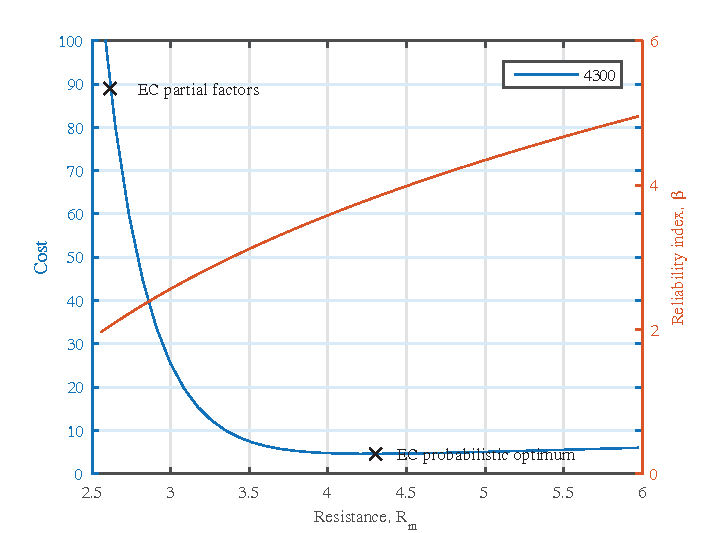
\includegraphics[width=0.7\textwidth]{cost_opti_ec_get_ratioeps_total.pdf}
	\caption{Total economic cost (blue) and reliability index (orange) as a function the mean resistance ($R_\mathrm{m}$); the designs obtained by partial factor and reliability based calculations are illustrated by a cross.}
	\label{fig:cost_opti_ec_total}
\end{figure}

\begin{figure}[htbp!] 
	\centering    
	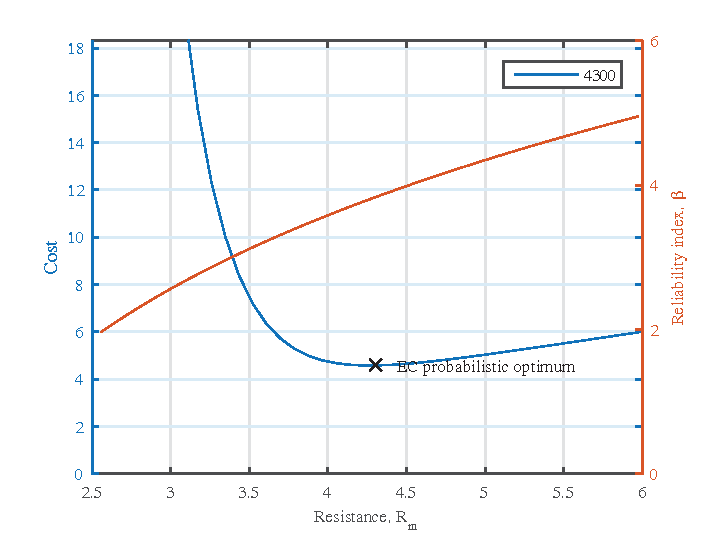
\includegraphics[width=0.7\textwidth]{cost_opti_ec_get_ratioeps_zoom.pdf}
	\caption{Same as Fig. \ref{fig:cost_opti_ec_total} but zoomed to the economic optimum.}
	\label{fig:cost_opti_ec_zoom}
\end{figure}


\subsubsection{Comparing Gumbel (EC) and BMA based optimum points}

\begin{figure}[htbp!] 
	\centering    
	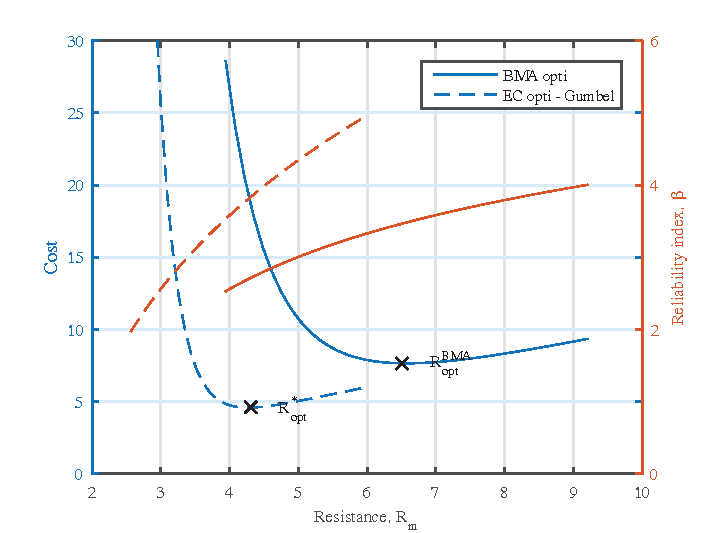
\includegraphics[width=0.7\textwidth]{cost_opti_compare_ec_bma.pdf}
	\caption{Optimum values with Gumbel and BMA models using the same ${C_{\mathrm{f}}}/{C_1}$ ratio.}
	\label{fig:cost_opti_ec_bma}
\end{figure}

Comparison of EC partial factor based design, EC cost optimization, both using Gumbel distribution and BMA cost optimization is summarized in Table \ref{tab:cost_opti_comp}.

% notes should be added
\begin{table}
\caption{Comparison of methods and models with different variable action model.}
\centering
\label{tab:cost_opti_comp}
\small
	\begin{threeparttable}
	\begin{tabular}{m{1cm} m{3cm} m{3cm} m{3cm}}
		\toprule
		  & EC partial factor, Gumbel  & EC opti, Gumbel & BMA opti \\
		\midrule
		$R_\mathrm{m}$ & 2.62 & 4.27 & 6.57  \\
		
		$\beta$ & 2.05\tnote{*} & 3.80\tnote{\textdagger} & 3.48 \\
		
		$c_\mathrm{tot}$ & 89.0 & 4.57 &  7.64 \\
		\bottomrule
	\end{tabular}
	\begin{tablenotes}
	    \item[*] assuming that $Q$ is Gumbel distributed.
	    \item[\textdagger] consequence of the initial assumption, Section ?.
	\end{tablenotes}
	\end{threeparttable}
\end{table}

\subsubsection{Reliability index for 1-year reference period}

\subsubsection{Comparing Gumbel and BMA models for different ${C_{\mathrm{f}}}/{C_1}$ ratios}

\begin{itemize}
	\item The difference between Gumbel and BMA economic optimal resistances is increasing with increasing $C_f/C_1$ ratio.
	\item RC2 and RC3 partial factors yield to design which is optimal for ${C_{\mathrm{f}}}/{C_1}$ ratio multiple order of magnitude smaller than the one calculated in Section ?? by inverse analysis.
	\item The optimal reli index varies significantly with the ${C_{\mathrm{f}}}/{C_1}$ ratio.
\end{itemize}


\begin{figure}[htbp!] 
	\centering    
	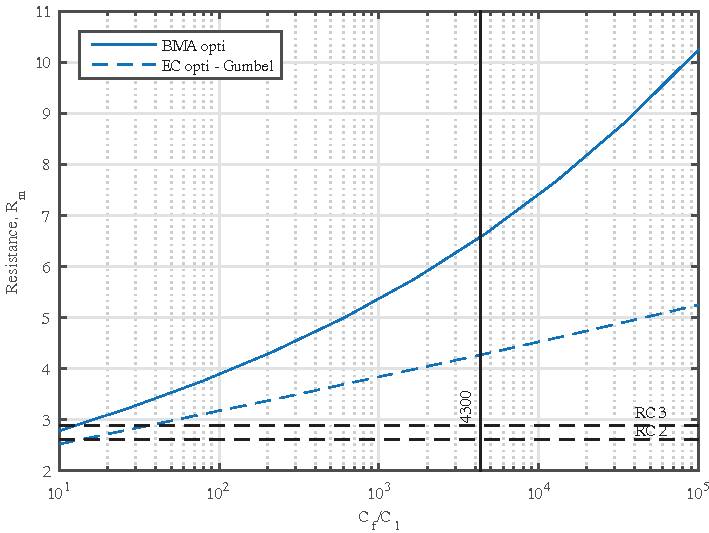
\includegraphics[width=0.7\textwidth]{comp_gumbel_bma_cf_c1_par.pdf}
	\caption{Mean resistances corresponding to economic optimum per different ${C_{\mathrm{f}}}/{C_1}$ ratios.}
	\label{fig:comp_gumbel_bma_res}
\end{figure}

\begin{figure}[htbp!] 
	\centering    
	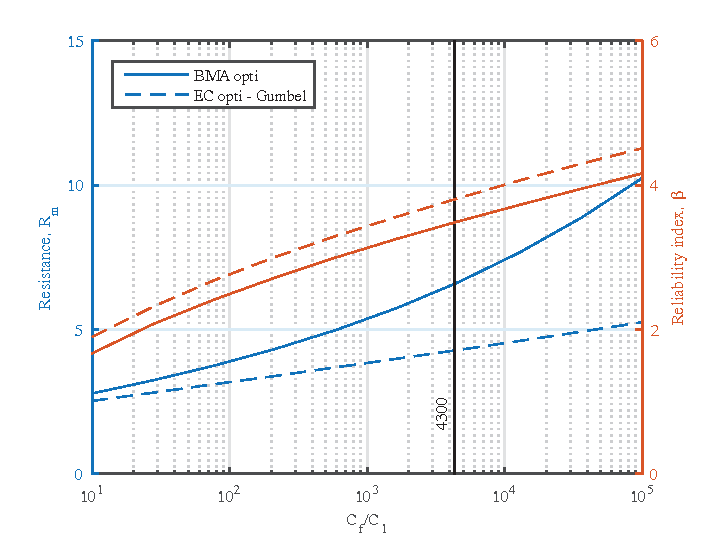
\includegraphics[width=0.7\textwidth]{comp_gumbel_bma_cf_c1_par_beta.pdf}
	\caption{Mean resistances and reliability indices corresponding to economic optimum per different ${C_{\mathrm{f}}}/{C_1}$ ratios.}
	\label{fig:comp_gumbel_bma_res_beta}
\end{figure}

\begin{figure}[htbp!] 
	\centering    
	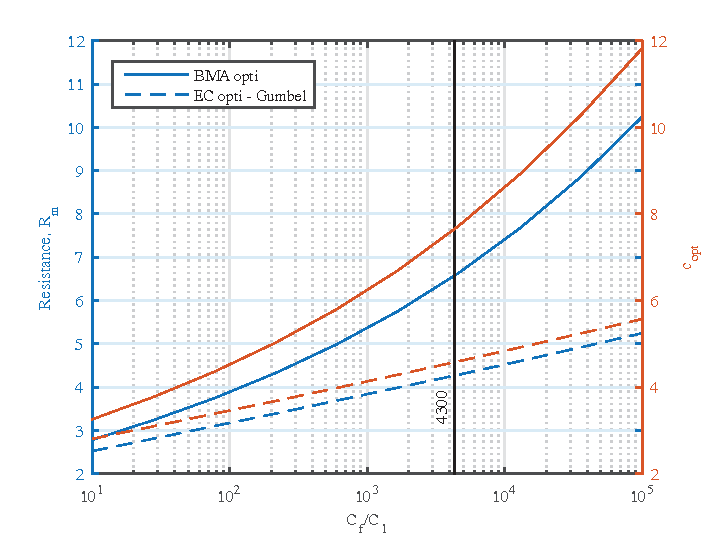
\includegraphics[width=0.7\textwidth]{comp_gumbel_bma_cf_c1_par_c_opt.pdf}
	\caption{Mean resistances and optimum costs corresponding to economic optimum per different ${C_{\mathrm{f}}}/{C_1}$ ratios.}
	\label{fig:comp_gumbel_bma_res_cost}
\end{figure}

\subsection{Partial factor for snow action}

Comments could be made on how the partial factor would change by incorporating parameter estimation uncertainty and by switching from Gumbel to GEV or other distribution types.
This a delicate question since it is well known that the current Eurocode recommendations do not provide the target reliability stipulated in \citep{EN0}. It is hard to separate the effects, though I believe it would convey interesting information.
Maybe Chapter \ref{cha:stat_unc} suits better for this analysis.

%\section{Extension to other random variables}

\section{Application example}

\section{Summary and conclusions}


\chapter{Effect of dependence structure}
\label{cha:copula}
% **************************** Define Graphics Path **************************
\ifpdf
    \graphicspath{{Chapter8/Figs/Raster/}{Chapter8/Figs/PDF/}{Chapter8/Figs/}}
\else
    \graphicspath{{Chapter8/Figs/Vector/}{Chapter8/Figs/}}
\fi

% **************************** Chapter Abstract ******************************
\leftskip=1cm
\noindent
\emph{In structural reliability the dependence structure between random variables is almost exclusively modeled by Gauss (normal or Gaussian) copula, however, this implicit assumption is typically not corroborated. Some studies -- from various disciplines -- indicate that the adopted copula function can have significant effect on the outcomes. This chapter focuses on time-variant reliability problems with continuous stochastic processes, which are collection of dependent random variables, and to our knowledge they are overwhelmingly modeled using Gauss copula in structural reliability. Therefore, the aim of this chapter is to quantify the impact of this copula assumption on failure probability. Three simple examples are studied considering bivariate Gauss, $t$, rotated Clayton, Gumbel, and rotated Gumbel copulas. The time-variant actions are modeled as stationary, ergodic, continuous stochastic processes, and the PHI2 method is adopted for the analyses. The calculations show that the copula function has significant effect on the failure probability. In the studied examples, application of Gauss copula can four times underestimate or even ten times overestimate the failure probabilities obtained by other copulas. The findings imply that the copula function should be inferred from observations or if not available, multiple copula functions and Bayesian model averaging is advocated to explore this uncertainty.}

\leftskip=0pt\rightskip=0pt

%****************************************************************************************
%****************************************************************************************
\section{Problem statement and the state of the art}
% Mirek ~ maybe leave it out for future), load combination is less important, focus on time-variant and time-invariant components

The problems in structural reliability require the integration of multidimensional joint probability distribution functions (Eq.\ref{eq:Pf_general}). Due to the scarcity of available information, the joint distribution is overwhelmingly given by its marginals and by a single parameter dependence measure between any two random variables. The typical dependence measure is the Pearson correlation coefficient, however, this single parameter does not uniquely determine the joint distribution function. This means that infinitely many joint distributions can be found to the prescribed marginals and correlation coefficient.

In structural reliability until recently it was a prevalent, implicit assumption that the dependence structure follows Gauss copula. However, some studies imply that this assumption is not justified by data, and can lead to severe under- or overestimation of failure probability. \citet{Tang2013geotech} showed that in geotechnical problems the function adopted to describe the dependence structure between cohesion and friction angle has significant effect on the failure probability. They demonstrated that the measurements are best described by Plackett copula, and the copula type might lead to an order of magnitude difference in the failure probability for slope stability. Further geotechnical engineering related studies arrived to similar conclusions \citep{Li2013, Tang2015}. A study on the impact of copulas on two-component parallel systems concluded that the tail dependence of copulas has significant effect on system reliability \citep{Tang2013system}. These results are particularly important for the current study, since the herein adopted PHI2 method formulates the time-variant reliability problem as a parallel system. Yet, there are important differences due to the nature of time-variant reliability problems, in this chapter: (\textit{i}) the system reliability calculation is only one step in the analysis; (\textit{ii}) the components have substantially different probabilities (failure and survival too); and (\textit{iii}) the component's failure probability is typically much lower than that of considered in the mentioned study.

Copulas are also widespread in many other fields, they are applied for instance for correlated stress-strength models \citep{Domma2013}, for risk assessment of dam overtopping considering bivariate distribution of flood peak and volume \citep{Requena2013}, for describing joint distribution of drought indices \citep{Madadgar2011}, for economic time series \citep{Patton2012}, and for modeling multivariate random variables in financial risk \citep{Donelly2010, Romano2002}.  All the referred studies draw attention to the importance of dependence structure modeling. Additionally, some show the grave consequences of Gauss copula assumption.
% (Aguilar-López et al. 2016)

To our knowledge, the impact of copulas on time-variant reliability problems has not yet been studied. The referred works suggest that in many cases the Gauss copula assumption is severely biased, thus the aim of this chapter is to quantitatively investigate the effect of copulas on time-variant reliability problems. We restrict our attention to stationary, ergodic stochastic processes and adopt the PHI2 method for the analysis.
This method is well suited for time-variant reliability questions where continuous stochastic processes are involved, since it reduces the problem to classical time-invariant problems, for which effective methods are available see, e.g. \citet{Ditlevsen2007}. The PHI2 method is an accurate, effective, and versatile compared to other time-variant techniques \citep{Renaud2002, Renaud2004, Baroth2011}. It has been successfully applied among others for the analysis of aging marine structures \citep{Mejri2011}, for degrading reinforced concrete beams \citep{Sudret2008rc}, for steel catenary riser subjected to extreme wave loading \citep{Perdrizet2008}, for adhesive bonded assemblies  \citep{Mejri2009}, and for floating wind turbines too \citep{Perdrizet2011}.

In Section~\ref{sec:stoch_proc}, the concept of stochastic processes and copula functions is briefly introduced and the adopted types are described. Thereafter, the PHI2 method and applied numerical techniques are outlined. Then, three simple examples are presented: (\textit{i}) parametric analysis of a minimal problem with a single stochastic process; (\textit{ii}) a simply supported beam with degrading resistance that also subjected to stochastic loading; and (\textit{iii}) a snow related stochastic problem, where copulas are fitted to observations.

%****************************************************************************************
%****************************************************************************************
\section{Stochastic processes}
\label{sec:stoch_proc}

Stochastic process is a sequence of random variables that are typically dependent and the strength of this dependence is the function of their distance. Here only time-continuous stochastic processes are considered where the distance is measured in time. Furthermore, the focus is restricted to stationary and ergodic processes. Under these assumptions, the stochastic process is fully characterized by its marginal distribution, autocorrelation function, and dependence (copula) function. The former describes the distribution of intensity in an arbitrary point in time. The autocorrelation function specifies the strength of dependence between random variables separated by a given time interval ($\Delta t$). This function applies only to the parameter that measures dependence, and the copula function is required to fully specify the dependence structure.

%****************************************************************************************
\subsection{Autocorrelation function}

Gaussian type autocorrelation function is the common choice in the literature. Herein, it is accompanied by Cauchy function to explore the effect of changing function type (Figure~\ref{fig:acorr_fun}). These two are applied in this work and defined as:
\begin{equation}
\label{eq:autocorr_gauss}
	{\rho _{{\mathrm{Gauss}}}}(\Delta t) = \exp \left( { - {{\left( {\frac{{\Delta t}}{{{\tau _\mathrm{F}}}}} \right)}^2}} \right) \text{\quad and}
\end{equation}
\begin{equation}
\label{eq:autocorr_cauchy}
	{\rho _{{\mathrm{Cauchy}}}}(\Delta t) = {\left( {1 + {{\left( {\frac{{\Delta t}}{{{\tau _\mathrm{F}}}}} \right)}^2}} \right)^{ - 2}}
\end{equation}
where:

\begin{tabular}{ll}
	$\tau_\mathrm{F}$ & correlation length; \\
	$\rho$ & Pearson correlation coefficient.
\end{tabular} \medskip

\noindent
Albeit the latter can express only linear dependence, it is applied here due to its ubiquity in the literature. Kendall's tau and Spearman's rho are more general single parameter measures. For instance, they are sensitive to any monotonic dependence, thus better candidates for dependence measure.

\begin{figure}[htbp!] 
	\centering    
	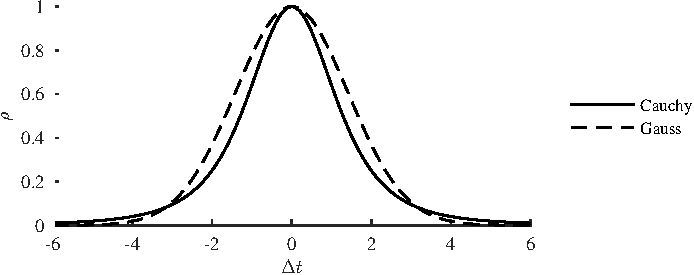
\includegraphics[]{autocorr_fun_illustration.pdf}
	\caption{Illustration of the considered autocorrelation functions.}
	\label{fig:acorr_fun}
\end{figure}

To allow direct comparison with published results and to utilize the more general Kendall's tau measure, the functions given in Eq.\ref{eq:autocorr_gauss} and \ref{eq:autocorr_cauchy} are kept and the following transformation is used:
\begin{equation}
\label{eq:tau_rho}
	\tau (\Delta t) = \frac{2}{\pi } \cdot \mathrm{asin}\left( {\rho (\Delta t)} \right).
\end{equation}
The equivalence of copulas is then set in terms of Kendall's tau values. Formula~\ref{eq:tau_rho} transforms between Pearson's rho ($\rho$) and Kendal's tau ($\tau$) for Gaussian and $t$ copulas, thus the connection to literature is established while allowing for easy extension to other copulas.

%****************************************************************************************
\subsection{Copula based dependence structure}
\label{sec:copula}

Copula is a multivariate probability distribution function with uniformly distributed marginals. It can be used to model the dependence between random variables with arbitrary marginal distributions \citep{Joe2014}. In this chapter, we deal mostly with bivariate distributions -- the formulas are given for that case -- though their extension to higher dimensions is straightforward. The copula function is expressed as:
\begin{equation}
\label{eq:copula_cdf}
	C\left( {{u_1},{u_2};\theta } \right) = {P}\left\{ {{U_1} \le {u_1},{U_2} \le {u_2}} \right\}
\end{equation}
where:

\begin{tabular}{ll}
	$C(.)$ & copula function; \\
	$\theta$ & copula parameter; \\
	$U_1, U_2$ & uniformly distributed random variables.
\end{tabular} \medskip  

\noindent
The copula function uniquely describes the dependence structure and it is independent of the marginals if those are continuous. Sklar's theorem establishes the connection between marginals, copula, and joint distribution \citep{Nelson2006, Marshall1996}:
\begin{equation}
\label{eq:sklar}
	{F_{X1X2}} = C\left( {{F_{X1}},{F_{X2}};\theta } \right)
\end{equation}
where:

\begin{tabular}{ll}
	$F_{X1}, F_{X2}$ & cumulative distribution functions of the marginals; \\
	$F_{X1X2}$ & the bivariate joint distribution.
\end{tabular} \medskip

\noindent
Copulas describe only the dependence structure of random variables, this separation of marginal and dependence is beneficial since in practice one has rarely full information about the joint distribution function, and it makes possible to separately infer the marginals and the copula.

In this chapter, Gauss, $t$, rotated Clayton, Gumbel, and rotated Gumbel copulas are adopted, all has a single parameter \citep{Nelson2006, Joe1997}. The copula functions with the range of the parameters are summarized in Table~\ref{tab:copula}. Furthermore, they are compared in Figure~\ref{fig:copula_cont}.

\begin{figure}[htbp!] 
	\centering    
	\includegraphics[]{5_copulas.pdf}
	\caption{Illustration of considered copula functions using bivariate density function contours. For all functions standard normal marginal distributions are used with 0.5 Kendall' tau.}
	\label{fig:copula_cont}
\end{figure}

The copula selection is partially motivated by their widespread use. Additionally, it is anticipated that these types cover broad range of possible functions, thus provide a representative picture about the impact of copulas on reliability. Theoretical upper and lower bounds exist for the copula functions, these are referred to as Fréchet-Hoeffding bounds \citep{Nelson2006} and they are also given in Table~\ref{tab:copula}.

Gauss (normal) and $t$ copulas belong to the elliptical family. Copulas within this family have density contours as concentric, constant eccentricity ellipses. Gumbel and Clayton copulas and their rotated alternatives belong to the Archimedean family. These are widely used due to their simple formulation and their great variety \citep{Nelson2006}. The Gumbel copula also belongs to the extreme copula family, which arises from extreme value theory, thus it can be used to model dependence between rare events \citep{Joe1997}. With the exception of Gauss copula, all considered copulas has tail-dependence, which roughly means that joint extremes are more likely than joint moderate values. Gumbel and rotated Clayton copulas have right-tale dependence, while rotated Gumbel copula has left-tail dependence. Both tails of $t$ copula exhibit tail dependence. These are also observable on the density contour plots in Figure~\ref{fig:copula_cont}, and might be of particular importance in structural reliability, which is governed by extremely rare events.

%\begin{landscape}
\begin{sidewaystable}[htbp!]
\caption{List of the considered copula functions, parameter ranges, and parameters as function of Kendall's tau ($\tau$).}
\centering
\label{tab:copula}
\small
	\begin{threeparttable}
    \begin{tabular}{llll}
    \toprule
    Name  & Copula function, $C(u_1,u_2;\theta)$ & Range of $\theta$ & $\theta(\tau)$ \\
    \midrule
    \rowcolor{lightgrey} Gauss  & ${\Phi _2}\left( {{\Phi ^{ - 1}}({u_1}),{\Phi ^{ - 1}}({u_2});\theta } \right)$ & [-1,1] & $\sin \left( {{\pi  \mathord{\left/
     {\vphantom {\pi  {2 \cdot }}} \right.
     \kern-\nulldelimiterspace} {2 \cdot }}\tau } \right)$  \\
     
     $t$  & ${t_2}\left( {{t^{ - 1}}({u_1};\nu ),{t^{ - 1}}({u_2};\nu );\theta } \right)$ & [-1,1] & $\sin \left( {{\pi  \mathord{\left/
          {\vphantom {\pi  {2 \cdot }}} \right.
          \kern-\nulldelimiterspace} {2 \cdot }}\tau } \right)$  \\
           
     \rowcolor{lightgrey} Gumbel  & $\exp \left( { - {{\left( { - \log {{({u_1})}^\theta } +  - \log {{({u_1})}^\theta }} \right)}^{{1 \mathord{\left/
       {\vphantom {1 \theta }} \right.
       \kern-\nulldelimiterspace} \theta }}}} \right)$ & [1,$\infty$] & ${1 \mathord{\left/
        {\vphantom {1 {\left( {1 - \tau } \right)}}} \right.
        \kern-\nulldelimiterspace} {\left( {1 - \tau } \right)}}$  \\ 
           
     rotGumbel-180°  & ${u_1} + {u_2} - 1 + \exp \left( { - {{\left( { - \log {{(1 - {u_1})}^\theta } +  - \log {{(1 - {u_2})}^\theta }} \right)}^{{1 \mathord{\left/
      {\vphantom {1 \theta }} \right.
      \kern-\nulldelimiterspace} \theta }}}} \right)$ & [1,$\infty$] & ${1 \mathord{\left/
              {\vphantom {1 {\left( {1 - \tau } \right)}}} \right.
              \kern-\nulldelimiterspace} {\left( {1 - \tau } \right)}}$  \\
    
     \rowcolor{lightgrey} rotClayton-180°  & ${u_1} + {u_2} - 1 + {\left( {\max \left\{ {{{\left( {1 - {u_1}} \right)}^{ - \theta }} + {{\left( {1 - {u_2}} \right)}^{ - \theta }} - 1;0} \right\}} \right)^{{{ - 1} \mathord{\left/
      {\vphantom {{ - 1} \theta }} \right.
      \kern-\nulldelimiterspace} \theta }}}$ & [-1,$\infty$]$\setminus \left\{ 0 \right\}$ & ${{2 \cdot \tau } \mathord{\left/
       {\vphantom {{2 \cdot \tau } {\left( {1 - \tau } \right)}}} \right.
       \kern-\nulldelimiterspace} {\left( {1 - \tau } \right)}}$  \\           
     
    lower bound, $C_\mathrm{sup}$  & $\max \left\{ {1 - 2 + {u_1} + {u_2};0} \right\}$ & -- & --  \\
    
    \rowcolor{lightgrey} upper bound, $C_\mathrm{inf}$  & $\min \left\{ {{u_1};{u_2}} \right\}$ & -- & --  \\
              
    \bottomrule
    \end{tabular}
    \begin{tablenotes}
    	\item $\Phi_2(.)$ and $\Phi(.)$  are the bi- and univariate standard normal cumulative distribution functions.
    	\item $t_2(.)$ and $t(.)$ are the bi- and univariate $t$ cumulative distribution functions with $\nu = 2$ degrees of freedom.
    	\item -- Not applicable/not available. 
   	\end{tablenotes}
   	\end{threeparttable}
\end{sidewaystable}
%\end{landscape}



%****************************************************************************************
%****************************************************************************************
\section{PHI2 method}

PHI2 method is an algorithm to solve time-variant reliability problems where (\textit{i}) a random variable is monotonically changing in time, e.g. degradation of material properties; and/or (\textit{ii}) a continuous time-varying process is involved. The algorithm originates from \citet{Hagen1991}, who formulated the calculation of the out-crossing rate as a two-component, parallel system reliability problem (Eq.\ref{eq:out_cross}).
Out-crossing occurs if a random variable or stochastic process is passing the limit state function from safe- to failure region. By definition, the out-crossing rate in time is given as \citep{Hagen1991}:
\begin{equation}
\label{eq:out_cross}
	{\nu ^ + }(t) = \mathop {\lim }\limits_{\Delta t \to 0} \frac{{P\left( {\left\{ {g(t) > 0} \right\}\bigcap {\left\{ {g(t + \Delta t) \le 0} \right\}} } \right)}}{{\Delta t}}
\end{equation}
where:

\begin{tabular}{ll}
	$\nu ^+$ & out-crossing rate; \\
	$g(.)$ & limit state function; \\
	$t$ & monotonically increasing parameter, typically time.
\end{tabular} \medskip

\noindent
Since in structural engineering out-crossings occur rarely, it is generally assumed that they can be described with a Poisson process \citep{Cramer1967}. After some algebra and simplification one can derive the formula that is widely used in structural reliability to calculate time-variant failure probability \citep{Melchers2002}:
\begin{equation}
\label{eq:P_f_t}
	{P_{\mathrm{f}}}(t) = {P_{\mathrm{f}}}(0) + \int\limits_0^t {{\nu ^ + }(\tau )}  \cdot {\mathrm{d}}\tau.
\end{equation}
The nominator in Eq.\ref{eq:out_cross} expresses the failure probability of a parallel system with correlated components. This system reliability problem inherits the copula assumption of the stochastic process. The correlation is typically estimated from the sensitivity factors obtained by first order reliability analysis (FORM) and then bivariate normal distribution is used to calculate the system failure probability \citep{Renaud2004}. Likely this is why the method is coined as PHI2 by \citet{Renaud2002}. However, the method is more general and not restricted to bivariate normal distribution, thus the naming is not fortunate. Nevertheless, it reflects well the overwhelming use of Gauss copulas in structural reliability. The application of Gauss copula in classical reliability methods such as FORM is usually referred to as Nataf transformation \citep{Liu1986, Nataf1962}.

It is known that the out-crossing rate given by Eq.\ref{eq:out_cross} is sensitive to the size of the time step ($\Delta t$), thus \citet{Sudret2008anal} derived an improved formula, which considerably mitigates this. Since it also relies on the Gauss copula assumption, the original, numerical derivation (Eq.\ref{eq:out_cross}) version is adopted here. To minimize the error, Sudret recommends the time step to be taken as 10\% of the correlation length ($\tau_\mathrm{F}$). Our analysis confirms this recommendation for Gauss copula with double precision calculation. However, for other copulas the results can be greatly sensitive to the chosen time step. To alleviate this problem multiprecision calculation -- quad or larger \citep{mct2016}  -- is adopted that yields to numerically stable results even for small time steps. For the examples in this chapter the range $\Delta t = \left( {{{10}^{ - 5}} \div {{10}^{ - 3}}} \right) \cdot {\tau _F}$  is found to have stable convergence: (\textit{i}) the time step is sufficiently small to accurately estimate the derivative (Eq.\ref{eq:out_cross}); and (\textit{ii}) the floating point representation is accurate enough to keep truncating errors low. Thus, for all calculations time step in this range is applied, the convergence and sensitivity to discretization are checked in each cases.

The system reliability problems emerging in PHI2 method are formulated with different copulas and solved by direct, numerical integration (DI). This approach is suited only for simple problems, such those considered in this chapter. For more complicated problems computationally more efficient methods would be needed such as FORM or SORM. Note, that these methods are almost solely implemented with Nataf transformation (Gauss copula) in the currently available research and commercial applications. They can be extended to elliptical copulas, since for these the physical variables can be transformed to a space where the search for the most probable point reduces to minimal distance search \citep{Lebrun2009}. However, to date, for other copula types no generalization of these methods is available, thus the application of non-elliptical copulas might be unmanageable.

%****************************************************************************************
%****************************************************************************************
\section{Example 1: simple time-variant problem}

First, a simple example is analyzed with a single continuous stochastic process ($S(t)$) and deterministic resistance ($R$). The limit state function is linear and expressed by Eq.\ref{eq:gfun_ex1}:
\begin{equation}
\label{eq:gfun_ex1}
	g(t) = R - S(t). 
\end{equation}
Using Eq.\ref{eq:out_cross}, the system failure probability ($P_\mathrm{f,sys}$), required in PHI2 method can be written as:
\begin{equation}
\label{eq:P_f_sys}
	{P_{{\mathrm{f,sys}}}} = {{P}}\left( {\left\{ {R - {S_1} > 0} \right\}\bigcap {\left\{ {R - {S_2} \le 0} \right\}} } \right).
\end{equation}
Where $S_1$ and $S_2$ are correlated random variables defined as:
\begin{equation}
\label{eq:S_def}
	{S_1} = S(t) \text{\quad and \quad} {S_2} = S(t + \Delta t). 
\end{equation}
Using Eq.\ref{eq:P_f_sys} and \ref{eq:sklar}, the failure probability of the parallel system can be expressed as:
\begin{equation}
\label{eq:P_f_sys_ex1}
	\begin{aligned}
		{P_{{\mathrm{f,sys}}}} &= {F_S}\left( R \right) - {F_{S1S2}}\left( {R,R} \right)\\
		 & = {P_{{\mathrm{s,comp}}}} - C\left( {{P_{{\mathrm{s,comp}}}},{P_{{\mathrm{s,comp}}}};\theta } \right)
	\end{aligned}
\end{equation}
where $P_\mathrm{s,comp}$ stands for the survival probability of a component and it corresponds to $1-P_\mathrm{f}(0)$. It can be seen from Eq.\ref{eq:P_f_sys_ex1} that for a given $P_\mathrm{s,comp}$ the system's failure probability is independent of the marginal distributions. Therefore, the stochastic process is sufficiently characterized by the autocorrelation function and by the copula, for the current purposes.

By specifying $P_\mathrm{s,comp}$ and the copula type, the system's failure probability can be calculated. Then by the finite difference formulation of Eq.\ref{eq:out_cross} and using Eq.\ref{eq:P_f_t} the time-variant reliability can be obtained. For this example, the time interval is taken as 50 years, and the autocorrelation length is $\tau_\mathrm{F} = 1/365$ year. First, Gaussian autocorrelation function is used.

The analyses are completed for various initial/component failure probabilities ranging from $10^{-10}$ to $10^{-6}$ with all five copulas having the same Kendall's tau for a particular set of input parameters. The results are represented as reliability indices in Figure~\ref{fig:beta_ex1}. Moreover, Figure~\ref{fig:pf_ex1} summarizes the time-variant failure probabilities and their normalized values.

\begin{figure}[htbp!] 
	\centering    
	\includegraphics[]{simple_example_beta.pdf}
	\caption{Reliability indices ($\beta$) and normalized reliability indices plotted against initial failure probability ($P_\mathrm{f}(0)$) for various copulas. DI refers to direct integration.}
	\label{fig:beta_ex1}
\end{figure}

\begin{figure}[htbp!] 
	\centering    
	\includegraphics[]{simple_example_Pf.pdf}
	\caption{Failure probabilities ($P_\mathrm{f}$) and normalized failure probabilities plotted against initial failure probability ($P_\mathrm{f}(0)$) for various copulas. DI refers to direct integration.}
	\label{fig:pf_ex1}
\end{figure}

From the figures it is clear that the copula type has significant effect on the failure probability. Compared with the widely used Gauss, the rotated Gumbel copula gives 3.1-3.9 times higher failure probability, the ratio is decreasing with decreasing initial failure probability. On the other hand, $t$, Gumbel, and rotated Clayton copulas yield to 0.09-0.33 times lower results than the Gauss copula; here too the ratio is decreasing with decreasing initial failure probability. Irrespectively of the copula type, the initial failure probability has no significant effect on the normalized results.

The calculations are repeated with other correlation lengths ranging from 0.1/365 to 100/365. It is found that the normalized results are only slightly affected by this change, even at maximum less than 2\% change is observed in failure probability. This can be explained by that (\textit{i}) the correlation between $S_1$ and $S_2$ is independent of $\tau_\mathrm{F}$ because $\Delta t$ is chosen as a fixed percentage of that; and (\textit{ii}) $P_\mathrm{f}(0)$ is typically much smaller than the second term in Eq.\ref{eq:P_f_t}. Indeed, the largest difference is observed when $P_\mathrm{f}(0)$ is comparable to the time-variant failure probability. In case of $\tau _\mathrm{F} = 1000/365$ for Gumbel copula, the normalized time-variant failure probability increases by 7\% compared to 1/365 year correlation length. The increase is 15\% for rotated Clayton copula.

Up to this point, all presented calculations correspond to Gaussian autocorrelation function. Switching to Cauchy function, the normalized time-variant failure probabilities -- with $\tau_\mathrm{F} = 1/365$ year correlation length -- change irrespectively of initial failure probability and of copula type. The ratio of normalized time-variant Cauchy and Gaussian failure probabilities is uniformly 1.41. It is solely influenced by the autocorrelation function.

In our case, the upper Fréchet-Hoeffding bound yields to zero up-crossing rate, while the lower bound gives infinitely large value. These can be shown using Eq.\ref{eq:P_f_sys_ex1} and Table~\ref{tab:copula}:
\begin{equation}
	\begin{split}
		\begin{aligned}
			{P_{{\mathrm{f,sys,inf}}}} &= {P_{{\mathrm{s,comp}}}} - {C_{\sup }}\left( {{P_{{\mathrm{s,comp}}}},{P_{{\mathrm{s,comp}}}}} \right) = 3 \cdot {P_{{\mathrm{s,comp}}}} - 1\\
			{P_{{\mathrm{f,sys,sup}}}} &= {P_{{\mathrm{s,comp}}}} - {C_{\inf }}\left( {{P_{{\mathrm{s,comp}}}},{P_{{\mathrm{s,comp}}}}} \right) = 0
		\end{aligned}
	\end{split}
		\begin{split}
			\begin{aligned}
				\xrightarrow[]{{\frac{{{\mathrm{d}}{P_{{\mathrm{f,sys}}}}(t)}}{{{\mathrm{d}}\Delta t}}}} \nu _{\inf }^ +  &= \infty \\
				\xrightarrow[]{{\frac{{{\mathrm{d}}{P_{{\mathrm{f,sys}}}}(t)}}{{{\mathrm{d}}\Delta t}}}} \nu _{\sup }^ +  &= 0.
			\end{aligned}
		\end{split}
\end{equation}
This means that the copula bounds convey no useful information; however, more importantly it implies that there are copula functions that yields to arbitrary large or arbitrary small out-crossing rates. Hence, compared with Gauss copula, arbitrary large error could be produced.

%****************************************************************************************
%****************************************************************************************
\section{Example 2: corroding beam}

The following example is adopted from \citet{Sudret2008anal}. It is a simply supported, corroding steel beam subjected to a time-variant load that is described by a continuous stochastic process (Figure~\ref{fig:corr_beam}). The original example is intended to illustrate the application of PHI2 method to solve a time-variant reliability problem and it implicitly adopted Gauss copula. Herein we extend the example by investigating the effect of copula function on out-crossing rate and reliability.

\begin{figure}[htbp!] 
	\centering    
	\includegraphics[]{corroding_beam_illustration_.pdf}
	\caption{Illustration of the corroding beam example.}
	\label{fig:corr_beam}
\end{figure}

The mechanical and probabilistic models (Table~\ref{tab:prob_models_corr_beam}) are the same as in the original example, solely the copula is varied that describes the dependence between the survival and failure of the structure between two ``close'' time instants.

\begin{table}[htbp!]
\caption{Probabilistic models for corroding beam example.}
\centering
\label{tab:prob_models_corr_beam}
\small
	\begin{threeparttable}
    \begin{tabular}{llll}
    \toprule
    Variable name  & Distribution & Mean & CV\\
    \midrule
    \rowcolor{lightgrey} Concentrated load, $S(t)$ [N]  & Normal & 3500 & 0.20  \\
    Yield strength, $\sigma_\mathrm{R}$ [MPa]  & Lognormal & 240 & 0.10  \\
    \rowcolor{lightgrey} Beam width, $b_0$ [mm]  & Lognormal & 200 & 0.05  \\
    Beam height, $h_0$ [mm]  & Lognormal & 40 & 0.10  \\
    \rowcolor{lightgrey} Unit weight, $\rho_\mathrm{st}$ [kN/$\mathrm{m}^3$]  & constant & 78.5 & --  \\
    Span, $L$ [m]  & constant & 5 & -- \\
    \bottomrule
    \end{tabular}
    \begin{tablenotes}
    	\item -- Not applicable.
    \end{tablenotes}
    \end{threeparttable}
\end{table}

The autocorrelation function of the stochastic process is Gaussian (Eq.\ref{eq:autocorr_gauss}), with correlation length of 1 day. The corrosion occurs uniformly on the surface of the beam and propagates linearly in time:
\begin{equation}
	b(t) = {b_0} - 2 \cdot \kappa  \cdot t \text{\quad and \quad} h(t) = {h_0} - 2 \cdot \kappa  \cdot t 
\end{equation}
where:

\begin{tabular}{ll}
	$t$ & time; \\
	$\kappa$ & corrosion rate, 0.05 mm/year.
\end{tabular} \medskip

\noindent
Taking into account the self-weight of the beam and the time-variant load ($S(t)$) the limit state function corresponding to the formulation of a plastic hinge at midspan is given by Eq.\ref{eq:gfun_corr_beam}:
\begin{equation}
\label{eq:gfun_corr_beam}
	\begin{aligned}
		g(t) &= {M_{\mathrm{R}}}(t) - \left( {{M_{\mathrm{G}}} + {M_S}(t)} \right)\\
		& = \frac{{b(t) \cdot h{{(t)}^2} \cdot {\sigma _{\mathrm{R}}}}}{4} - \left( {\frac{{{\rho _{{\mathrm{st}}}} \cdot {b_0} \cdot {h_0} \cdot {L^2}}}{8} + \frac{{S(t) \cdot L}}{4}} \right).
	\end{aligned}
\end{equation}
In accordance with the original example, the self-weight is assumed to be time-invariant, although the cross-section's dimensions are decreasing in time. The design life of the beam is assumed to be 20 years.

The time-variant reliability problem is solved with copulas listed in Table~\ref{tab:copula}; the corresponding out-crossing rates and normalized out-crossing rates in time are shown in Figure~\ref{fig:outcross_ex2}. In case of Gauss copula, besides the direct numerical integration (DI) the calculations are also carried out by FORM. In the latter, the correlation between the two components (Eq.\ref{eq:out_cross}) is estimated from the angle between corresponding FORM hyperplanes \citep{Ditlevsen1979bounds}. The small difference between FORM and numerical integration outcomes is attributed (\textit{i}) to the non-linearity of limit state function; and (\textit{ii}) to the approximate correlation coefficient used in FORM. The results confirm the applicability of FORM to approximate the reliability.

\begin{figure}[htbp!] 
	\centering    
	\includegraphics[]{Sudrets_beam_log_nu.pdf}
	\caption{Out-crossing rates ($\nu ^+$) and normalized out-crossing rates in time for various copulas. DI refers to direct integration.}
	\label{fig:outcross_ex2}
\end{figure}

Figure~\ref{fig:outcross_ex2} shows considerable differences in out-crossing rates for different copulas. Compared with the Gauss-DI solution, the rotated Gumbel copula gives about 1.8 times larger rates, while other copulas lead to smaller rates. The largest reduction is observed for rotated Clayton copula, which is 0.25 times that of the Gauss copula. It can be also observed that normalized out-crossing rates vary only slightly in time.

Figure~\ref{fig:Pf_ex2} and Figure~\ref{fig:beta_ex2} illustrate the time-variant failure probabilities and reliability indices, respectively. The former follows well the trend observed in out-crossing rates, which is as quasi-constant ratio in time. In Figure~\ref{fig:Pf_ex2}, it can be seen that the normalized ratios per copula function is very close to that of the out-crossing rates, with the exception of $t=0$ time instant, where the out-crossing rate is not taken into account. The figures also indicate that the two degrees of freedom $t$ copula leads to similar results as of Gumbel copula. Compared with the Gauss copula with direct integration, the largest ratios in failure probabilities are 1.1 and 1.8 for Gauss-FORM and rotated Gumbel copulas, respectively. The smallest ratios are 0.7, 0.5, and 0.3 for $t$, Gumbel, and rotated Clayton copulas, respectively. The increasing difference in reliability indices with increasing time is attributed to the nonlinear transformation between failure probability and reliability index.

\begin{figure}[htbp!] 
	\centering    
	\includegraphics[]{Sudrets_beam_log_Pf.pdf}
	\caption{Failure probabilities ($P_\mathrm{f}$) and normalized failure probabilities in time for various copulas. DI refers to direct integration.}
	\label{fig:Pf_ex2}
\end{figure}

\begin{figure}[htbp!] 
	\centering    
	\includegraphics[]{Sudrets_beam_beta.pdf}
	\caption{Reliability indices ($\beta$) and normalized reliability indices for various copulas. DI is referring to direct integration.}
	\label{fig:beta_ex2}
\end{figure}

All the presented results are from analyses using Gaussian autocorrelation function. The calculations are repeated with Cauchy autocorrelation function and the outcomes show that the change in out-crossing rate is independent of the copula type and time. The ratio of out-crossing rate obtained by using Cauchy and Gaussian autocorrelation functions is 1.41. This considerable effect is also rarely acknowledged in the literature, where the Gaussian autocorrelation function is prevalent. This ratio is inherited by the time-variant failure probability since the initial failure probability is negligible compared to the term involving the out-crossing rate (Eq.\ref{eq:P_f_t}).

%****************************************************************************************
%****************************************************************************************
\section{Example 3: generic structure subject to snow load}
\label{sec:copula_snow}

In this example a time-variant reliability problem is studied, where the stochastic process is inferred from observations. Maximum likelihood method (Section~\ref{subsec:point estiamtes}) is chosen for parameter estimation. However, the calculation of the full likelihood is computationally demanding -- often numerically intractable -- even for moderately large datasets due to the need to evaluate high-dimensional, multivariate distributions. Thus, it is often replaced with pairwise likelihood that requires only bivariate distributions and shares the same properties as the full likelihood based estimator except its loss of efficiency \citep{PadoanRibatetSisson2010}. This pairwise approach is also applied for spatial modeling such as temperature extremes in Switzerland \citep{Ribatet2012} and adopted herein too. The formulation of the pairwise likelihood function is given as:
\begin{equation}
	{L_{\mathrm{p}}}\left( {{\bf{x}};{\bf{\theta }}} \right) = \prod\limits_{i < j} {p\left( {\left[ {{x_i},{x_j}} \right];{\bf{\theta }}} \right)}.
\end{equation}
Ground snow observations in the form of snow water equivalent are selected for the representative lowland location of Budapest in the Carpathian Region. The data are from the CarpatClim database and available in 10~km spatial and 1-day maxima temporal resolution \citep{Szalai2013}. Budapest (19.1°E, 47.5°N) is characterized by intermittent snow cover, i.e. couple of snowfalls followed by often complete melting. The analyzed sample is extracted using the following principles:
\begin{itemize}
	\item peaks are extracted from daily maxima;
	\item from two peaks separated by four or less days the smaller one is removed;
	\item each winter season is treated as a single unit because snowfalls are clustered over a few months;
	\item if only a single peak occurs in a season its likelihood is calculated from the univariate marginal.
\end{itemize}
This means that a sequence of peaks is obtained for each winter seasons that are assumed to be independent. However, peaks within the same season are treated as realizations of a time-continuous stochastic process, thus they are dependent. The extracted sequence of peaks along with daily maxima are illustrated in Figure~\ref{fig:peak_sample_ex3} for five consecutive years.

\begin{figure}[htbp!] 
	\centering    
	\includegraphics[]{sample_&_peaks.pdf}
	\caption{Illustration of extracted peaks from daily snow water equivalent (SWE) maxima over five consecutive years.}
	\label{fig:peak_sample_ex3}
\end{figure}

Note that this is a somewhat arbitrary approach and the sample could be extracted many different ways. However, this deemed sufficient to illustrate the effect of copulas inferred from data. In average five peaks are present for a given winter season and in total there are 249 peaks for the 49 seasons. Gauss and Cauchy autocorrelation functions, and Gauss, $t$, Gumbel, rotated Gumbel, and rotated Clayton copulas are considered. Additionally, three marginal distributions are used: Gauss, Lognormal, and Gumbel.

For each autocorrelation-marginal-copula triplet three parameters are inferred: two parameters of the marginal and the correlation length. Separate inference of the marginal and copula is not possible due to nature of the problem, thus the parameters are estimated simultaneously.

Akaike information criterion (AIC, Eq.\ref{eq:AIC}) is calculated for each triplet. Then pooling is made for each autocorrelation-marginal sets, where a set is composed of the copulas as candidate models. This pooling is explained by the large difference in AIC (>100) between models with different marginal function. The related Akaike weights ($w$, Eq.\ref{eq:Akaike_weight}) are visually compared in Figure~\ref{fig:akaike_ex3}. It shows that -- with the exception of Gauss autocorrelation-Gumbel marginal pair -- Gumbel copula performs significantly better than the other considered copulas.

\begin{figure}[htbp!] 
	\centering    
	\includegraphics[]{akaike_weights.pdf}
	\caption{Akaike weights for autocorrelation-marginal pools. A pool is formed by a particular autocorrelation function (Gauss, Cauchy) and by a particular marginal distribution (Gauss, Lognormal, Gumbel), and the six copula functions provide the candidate models.}
	\label{fig:akaike_ex3}
\end{figure}

In most cases, the Cauchy autocorrelation function provides significantly better fit ($\Delta \mathrm{AIC} > 5$) than the Gauss using the same type of copula and type of marginal. The only exception is the rotated Clayton copula for which Gauss autocorrelation function is slightly better. The marginal distribution type has substantial effect on the fit, it can yield to over 100 difference in AIC. Lognormal provides the best fit, followed by Gumbel and Gauss.
The outstanding performance of Gumbel copula implies that extreme copulas might suit better for describing dependent extremes, this conjecture is also supported by the extreme value theory. Furthermore, by using extreme $t$ copula with two degrees of freedom even better fit is obtained than that of Gumbel.

To explore the effect on time-variant reliability the inferred stochastic models are used in a simple reliability problem characterized by the following limit state function:
\begin{equation}
	g(t) = R - \left( {G + S(t)} \right).
\end{equation}
The properties of the involved probabilistic models are summarized in Table~\ref{tab:prob_models_snow_stoch}.

\begin{table}[htbp!]
\caption{Marginal distribution of random variables for stochastic snow load example.}
\centering
\label{tab:prob_models_snow_stoch}
\small
	\begin{threeparttable}
    \begin{tabular}{llll}
    \toprule
    Variable name  & Distribution & Mean & CV \\
    \midrule
    \rowcolor{lightgrey} Resistance, $R$  & Lognormal & 250 & 0.10  \\
    Permanent action, $G$  & Normal & 60 & 0.07  \\
    \rowcolor{lightgrey} Snow maxima, $S(t)$  & Normal, Lognormal, Gumbel & \tnote{*} & \tnote{*}  \\
    \bottomrule
    \end{tabular}
    \begin{tablenotes}
    	\item[*] Depends on the applied autocorrelation-marginal-copula triplet.  
   	\end{tablenotes}
   	\end{threeparttable}
\end{table}

For comparison, the out-crossing rates are calculated for each triplet and presented in a normalized form in Figure~\ref{fig:norm_nu_ex3}. For each marginals the out-crossing rates are normalized with that of the corresponding Gauss copula. The same trend is observed for all marginals. Using Gauss copula the largest underestimation of out-crossing rate is 8 times, while the largest overestimation is 3 times. Neither of these are corresponding to Gumbel copula, which yields to 4.2, 2.9, and 3.5 times smaller out-crossing rates for Gauss, Lognormal, and Gumbel marginals, respectively. Figure~\ref{fig:norm_nu_ex3} conceals the multiple order of difference between out-crossing rates of different marginals. Although it is low importance now as we are interested in the effect of copula functions. The effect of replacing the Gauss autocorrelation with Cauchy function yields to similar results as observed in previous examples. The ratio of corresponding Cauchy and Gauss out-crossing rates is uniformly about 1.4.

\begin{figure}[htbp!] 
	\centering    
	\includegraphics[]{normalized_nu_p.pdf}
	\caption{Normalized out-crossing rates for Gauss autocorrelation function. For each marginals (Gauss, Lognormal, Gumbel) the out-crossing rates are normalized with that of the corresponding Gauss copula. DI refers to direct integration.}
	\label{fig:norm_nu_ex3}
\end{figure}

\section{Application example: Eiffel-hall of Budapest}
In Section~\ref{sec:copula_snow} a generic structure is analyzed, which is located at the site of Eiffel-hall. Herein the same location -- thus same snow action -- but the structure of the Eiffel-hall is investigated. The structure is introduced in Annex~\ref{sec:eiffel}, here only the essential details, which are required to interpret the results, are provided. The stochastic snow models fitted in the preceding section is used in the analysis. Only Gaussian autocorrelation function and Gumbel marginal distribution are considered. The wind action is represented by a distribution function corresponding to 50 years reference period. The out-crossing rates -- calculated by direct numerical integration -- are summarized in Table~\ref{tab:eiffel_nu_p}. Compared with Gauss copula, the largest difference is observed for Gumbel copula, which yields to about three times smaller out-crossing rate. Figure~\ref{fig:akaike_ex3} shows that for the inputs the $t$ copula provides the best fit, which leads to 40\% smaller out-crossing rate than that of the Gauss. The effect of copula function type is smaller than in previous examples, though it is still considerable.

\begin{table}[htbp!]
\caption{Out-crossing rates for Eiffel-hall considering Gauss autocorrelation function and Gumbel marginal distribution.}
\centering
\label{tab:eiffel_nu_p}
\small
    \begin{tabular}{llllll}
    \toprule
    Parameter  & Gauss & $t$ (dof=2) & Gumbel & rotGumbel-180° & rotClayton-180°\\
    \midrule
    \rowcolor{lightgrey} $\nu^+$ [$\cdot 10^{-3}$]  & 1.18 & 0.737 & 0.403 & 2.22 & 0.794  \\
    $\nu^+/\nu_\mathrm{Gauss}^+$  & 1.00 & 0.622 & 0.340 & 1.87 & 0.671 \\
    \bottomrule
    \end{tabular}
\end{table}

%****************************************************************************************
%****************************************************************************************
\section{Discussion}

Dependence structure (or copula function) uncertainty belongs to probability model selection uncertainty. Thus, from mathematical point of view the issue is very similar to distribution selection uncertainty, which is treated in Chapter~\ref{cha:stat_unc}. The same considerations apply here as well: typically there are insufficient data to identify the true model, copula function. Hence, for normal structures agreement on the copula function is recommended, and for safety critical structures Bayesian model averaging is advocated to account for copula type uncertainty.

For non-Gaussian copulas direct integration is used here and typically quad or larger  precision calculation is required to achieve convergence. Efficient algorithms, such as FORM, are currently only available for elliptical copulas, additional research would be needed to extend existing or develop new methods for other copulas. Thus, this poses a limitation on incorporation of copula function uncertainty in probabilistic analysis.

%****************************************************************************************
%****************************************************************************************
\section{Summary and conclusions}

In this chapter the effect of the dependence structure between random variables is analyzed on the failure probability of structures. Copula function is adopted to describe the dependence and the emphasis is placed on time-variant reliability using PHI2 method. The analysis of three simple examples -- considering Gauss, $t$, rotated Clayton, Gumbel, and rotated Gumbel copulas -- reveal:
\begin{itemize}
	\item The applied dependence structure has significant effect on time-variant reliability. The prevalently applied Gauss copula assumption can 4 times underestimate or even 10 times overestimate failure probabilities obtained by other adopted copulas.
	\item For a simple case (Example 1), it is demonstrated that by an appropriate choice of copula function arbitrary large error can be produced in out-crossing rate, compared with that of the Gauss copula.
	\item The correlation length of stochastic process and initial failure probability have minor effect on the ratio of the Gauss and other copula results.
	\item The autocorrelation function has considerable effect on the time-variant failure probability. The ratio of normalized time-variant Cauchy and Gaussian failure probabilities is uniformly 1.41. It is solely influenced by the autocorrelation function.
	\item Analysis of ground snow observations implies that extreme copulas, such as Gumbel, fit significantly better to dependent snow extremes than Gauss copula. The Gumbel copula can yield to 4 times lower out-crossing rate than that of Gauss.
\end{itemize}
	
To our knowledge the copula and autocorrelation effects have not yet been studied previously and the findings provide a novel insight into time-variant problems.
The results also give indication about whether a particular part of the mechanical or probabilistic model is worth of refinement, if the actual dependence structure is largely unknown.

If observations are available, the actual dependence structure should be inferred, and in case of limited information, multiple copula functions should be used to quantify the related uncertainty. Model averaging (Annex~\ref{subsec:model_averaging}) provides a viable approach to rigorously account for this uncertainty. In reporting of reliability analyses, the dependence structures, namely the adopted copulas should also be reported to give full description of the probabilistic model and to allow reproducibility.
\chapter{Summary and conclusions}
\label{cha:summary}
% **************************** Define Graphics Path **************************
\ifpdf
    \graphicspath{{Chapter9/Figs/Raster/}{Chapter9/Figs/PDF/}{Chapter9/Figs/}}
\else
    \graphicspath{{Chapter9/Figs/Vector/}{Chapter9/Figs/}}
\fi

% **************************** Chapter Abstract ******************************
\leftskip=1cm
\noindent
%\emph{This final chapter reviews the completed study from a broader perspective and recapitulates the main conclusions along with practical recommendations. Furthermore, theses are formulated, and novelties and limits of the study are highlighted.}
\emph{This final chapter provides a summary and it recapitulates the main conclusions along with practical recommendations. Furthermore, theses are formulated, and novelties and limits of the study are highlighted.}

\leftskip=0pt\rightskip=0pt

%****************************************************************************************
%****************************************************************************************
\section{Purpose and significance of the study}

The aim of this thesis is to subtly adjust the existing imbalance between probabilistic and physical models in civil engineering. To this end, it deals with issues related to probabilistic models and it aims to explore neglected effects and to provide improved probabilistic analysis to capture them.  Extreme ground snow load is selected as a vehicle of illustration, though the investigated issues are present for most random variables. The main contributions are as follows:
\begin{itemize}
	\item This study explores commonly neglected or underappreciated effects in structural reliability; these are: statistical uncertainty, measurement uncertainty, long-term trends, and dependence structure.
	\item Existing methods are transfered, adapted and applied from other fields to solve civil engineering issues. Some of these are rarely or have not been used before for issues considered here. These serve as reference since they are able to capture the neglected effects in current approaches.
	\item It is demonstrated that the neglect of the examined factors can lead to an order of magnitude underestimation of failure probability. Recommendations are made on how and when to incorporate them in probabilistic analysis.
\end{itemize}

The results are applicable to probabilistic analysis of structures and to codification as well. They bear significance especially for safety critical structures, such as nuclear power plants, where probabilistic risk analysis is prescribed. The findings provide improved insight into probabilistic analysis of snow extremes and into their effect on structural reliability.

%Although it shares many common aspects with other fields where statistical and probabilistic analyses are applied, e.g. sociology, meteorology, electrical engineering, there is an important difference in respect of magnitude of probabilities in which civil engineers are typically interested. Failure probabilities in civil engineering are typically in the range of $10^{-3}-10^{-6}$, which makes it  

%Application of methods developed in mathematical statistics and probability theory to civil engineering problems. Some neglected or inadequately addressed questions are answered using these methods. Strictly speaking no original idea is added just transferring and applying probabilistic methods to civil engineering problems.
%
%The main contribution of this study is that it explores commonly neglected or underappreciated effects in structural reliability these are: statistical uncertainty, measurement uncertainty, long-term trends, and dependence structure. These effects are demonstrated through extreme snow events, although present for all random variables. We argue that these could and should be incorporated or indicated in reliability studies since their neglect can introduce systematic bias. This not only violates one basic requirement in probability analysis\footnote{One of Jaynes' fundamental desideratum \citep{Jaynes2003} and Der Kiureghian requirements \citep{Kiureghian1989}.}
%
%An honest approach requires the appreciation of 
%The challenge is somehow similar to observational data analysis in health care, where systematic bias can lead to unreliable outcomes. With the increase of computational power and decrease of cost we expect large increase of data in civil engineering as well, e.g. cheap sensors providing continuous data and the my , although as the example of health care data analysis show we can expect additional challenges.

%We argue that these could and should be incorporated or indicated in reliability studies since their neglect can introduce systematic bias. This not only violates one basic requirement in probability analysis One of Jaynes' fundamental desideratum \citep{Jaynes2003} and Der Kiureghian requirements \citep{Kiureghian1989}.

%****************************************************************************************
%****************************************************************************************
\section{Recapitulation of main conclusions}

The main conclusions emphasizing the contributions\footnote{In accordance with the requirements of the Vásárhelyi Pál Doctoral School, the \mynote{alleged}contributions of the candidate are organized into theses. These are formulated to comply with the unwritten rules of the School. One of which is that the theses are to be written in first person singular.} of this work are presented as responses to the questions posed in Section~\ref{sec:prob_state}. The responses are identically structured and divided into subsections: previous works and current practice, methods, novelty, scope and limit, and thesis. Although the proposed practical recommendations constitute novelties they are not listed among them as they are presented at the theses. The assertions about current practice, previous works, and novelty of the answers are not absolute statements. The expression: \textit{to the best knowledge of the candidate} should be put in front of each.

%******************************************************************************************
%******************************************************************************************
\subsection{Distribution of annual ground snow maxima}

\textit{Which distribution function is the ``best'' to model ground snow extremes? What constitutes an appropriate model?}

\subsubsection{Previous works, current practice}
Consensus is missing on the appropriate model for annual ground snow maxima among reliability experts. Gumbel and three-parameter Lognormal distributions are widespread in Europe, while two-parameter Lognormal is typical in the USA. Often instead of a general rationale, prescriptions are provided thus adaptation to local conditions can be cumbersome.

\subsubsection{Methods}
Method of moments, frequentist, and Bayesian techniques are adopted for inference of distribution parameters. Visual checks and information theory based goodness-of-fit measures are used to identify the ``best'' performing distribution type. Gumbel, Generalized extreme value, two-parameter Lognormal, and three-parameter Lognormal distributions are considered.

\subsubsection{Novelty}
Advanced statistical analyses are performed on snow water equivalent annual maxima in the Carpathian Region, for example information theory based measures are used for model comparison. Application of many of these are novel compared with the typically adopted approaches and it allows for judging the merits and performance of the latter. In the spirit of open and successive research, posterior distributions and an online, open-source, interactive snow map are provided to facilitate cooperation between neighboring countries.

\subsubsection{Scope and limits}
The used methods, developed codes and applications are easily adaptable to other climatic actions. Limitations are that solely annual block maxima, limited number of distribution functions, and only three statistical techniques are considered. 

%.................................................................
% DISTRIBUTION
\begin{center}
	\noindent\rule[0.5ex]{0.5\linewidth}{0.5pt} \\[10pt]
	\textbf{Thesis I} \hfill \\[13pt]
\end{center}
%\end{center}
I statistically analyzed the ground snow water equivalent data of about 6000 grid points in the Carpathian Region covering 49 winter seasons from 1961 to 2010. I fitted multiple distribution types to the annual snow maxima that are extracted from daily observations. Based on extensive statistical analysis:
\begin{enumerate}[leftmargin=*, align=left, labelwidth=*]
	\item[\textbf{I/a}] I demonstrated that mountains and highlands are better represented by Weibull, while lowlands by Fréchet distribution compared with the currently standardized Gumbel model recommended in Eurocode and used in Hungary. I showed that the Gumbel model often appreciably underestimates the snow maxima of lowlands and thus overestimates structural reliability. The Lognormal model typically performs even worse than the Gumbel. From the considered distributions, based on reliability, empirical (data-driven), and theoretical considerations Weibull distribution is recommended for mountains and highlands, and Fréchet for lowlands.
	
	\item[\textbf{I/b}] I determined the posterior distribution of the characteristics of snow maxima for representative areas in the region. These can be used as prior information for regions with similar conditions. Furthermore, I created an open-source, online, interactive snow map for the Carpathian Region. It can be used to obtain characteristic ground snow load and to check exceptional ground snow load with 10~km spatial resolution. 
\end{enumerate}

\citep{RozsasAMM2016, RozsasESREL2015, VighTO2016, RozsasIABSE2015}
%VighTO2016

%******************************************************************************************
%******************************************************************************************
\subsection{Effect of statistical uncertainties}

\textit{How large is the effect of statistical uncertainties on structural reliability? Is their neglect reasonable? How should these uncertainties be taken into account?}
 
\subsubsection{Previous works, current practice}
Statistical uncertainties are routinely neglected in reliability analyses, i.e. point 
estimates of distribution parameters are used for representative fractiles and in 
probabilistic models. For example the background research document on snow loads of Eurocode completely ignores this uncertainty.

\subsubsection{Methods}
Frequentist and Bayesian approaches are applied to quantify parameter estimation and model selection uncertainties. The former is accounted for by uncertainty intervals and the latter is by model averaging. Bayesian posterior predictive distribution is used to integrate parameter estimation uncertainty into failure probability. Multiple examples with extensive parametric analyses are performed to explore the effect of neglecting statistical uncertainties.

\subsubsection{Novelty}
%Although precursors can be found in the civil engineering literature, these are based on rather arbitrary rules.
Systematic, rigorous analysis on the effect of statistical uncertainties on representative fractiles and on structural reliability has not yet been performed. Drawing attention to the severe underestimation of failure probability using current approaches provides novel insights.
 
\subsubsection{Scope and limits}
Although the numerical results and conclusions are confined to limited parameter range and are mainly focused on ground snow extremes, the adopted techniques are not restricted to the considered problem and can be utilized for other random variables, phenomena as well, such as floods and wind loads.
 
\begin{center}
	\noindent\rule[0.5ex]{0.5\linewidth}{0.5pt}
	\item[\textbf{Thesis II}] \hfill
\end{center}
%.................................................................
% STAT UNCERTAINTY 
I analyzed the effect of statistical uncertainties (parameter estimation and model selection uncertainties) in annual ground snow maxima on representative fractiles and on reliability. These are prevalently neglected in current civil engineering practice though inevitably present due to data scarcity.
\begin{enumerate}[leftmargin=*, align=left, labelwidth=*]
	\item[\textbf{II/a}] I showed that the neglect of parameter estimation uncertainty can lead to considerable (20\%) underestimation of representative fractiles. Furthermore, the applied distribution type (model selection uncertainty) has larger effect on representative fractiles than the parameter estimation uncertainty. Two-parameter Lognormal, three-parameter Lognormal, Gumbel, and Generalized extreme value distributions are considered.
	
	\item[\textbf{II/b}] Using reliability analyses, I demonstrated that the neglect of statistical uncertainties can even lead to multiple order of magnitude underestimation of failure probability. %This also means that the standards, which overwhelmingly neglect this uncertainty for load effects, provide lower reliability level than claimed.
	I illustrated that the use of ``best'' point estimates, such as maximum likelihood or method of moments estimates, are not conservative from reliability point of view. They can lead to practically significant underestimation of failure probability. Based on these findings, I made recommendations on the treatment of statistical uncertainties for normal and safety critical structures. Furthermore, I recommend the use of Bayesian posterior predictive distribution in reliability analysis and I advocate model averaging to account for model selection uncertainty.
\end{enumerate}

\citep{RozsasEpistemic2014, RozsasESREL2015, RozsasIABSE2015, RozsasMM2015, RozsasTVSB2015, RozsasIdojaras2016}


%******************************************************************************************
%******************************************************************************************
\subsection{Effect of measurement uncertainty}

\textit{How measurement uncertainty should be taken into account and propagated to structural reliability? Is the current practice, which neglects it, acceptable from reliability point of view? Is its effect on failure probability practically significant?}

\subsubsection{Previous works, current practice}
Observations are inevitably contaminated with measurement uncertainty, which is a significant source of uncertainty in some cases. In reliability analysis, probabilistic models are typically fitted to measurements without considering this uncertainty. The statistical approach to this problem is applied in astronomy, econometrics, biometrics, etc., however, not in civil engineering.

\subsubsection{Methods}
Statistical and interval based approaches are proposed to quantify and to propagate measurement uncertainty. These are critically compared by analyzing ground snow measurements, which are often affected by large measurement uncertainty. It is propagated through the mechanical model of a generic structure to investigate its effect on reliability.

\subsubsection{Novelty}
The conducted measurement uncertainty analyses represent novelty both in methods and in results, i.e. demonstrating their practical significance and the inadequacy of current practice. Mathematically sound statistical and interval based approaches are adapted from statistics and computational science. Their application to measurement uncertainty in civil engineering is novel.

\subsubsection{Scope and limits}
Although the study is limited by the considered distribution types (Normal, Lognormal, Gumbel), reality-observation links (additive, multiplicative), and parameter ranges (coefficient of variation 0.2-0.6), it covers many practically relevant random variables. The presented approaches and algorithms can be easily used for other distribution types and measurement error structures. An additional limitation of the study is that measurement uncertainty is considered only for the dominant variable action. Furthermore, the effect of sample size should be analyzed in future studies.

\begin{center}
	\noindent\rule[0.5ex]{0.5\linewidth}{0.5pt}
	\item[\textbf{Thesis III}] \hfill
\end{center}
%.................................................................
% MEASUREMENT UNCERTAINTY
I analyzed the effect of measurement uncertainty in annual ground snow maxima on structural reliability, which is typically neglected in civil engineering. I proposed statistical and interval analysis based approaches and concluded that:
\begin{enumerate}[leftmargin=*, align=left, labelwidth=*]
	\item[\textbf{III/a}] Measurement uncertainty may lead to significant (order of magnitude) underestimation of failure probability. Ranges of the key parameters are identified where measurement uncertainty should be considered. I derived these from analysis of Normal, Lognormal, and Gumbel distributions with coefficient of variation ranging from 0.2 to 0.6 and with various extents of measurement uncertainty (0-10\% of mean of annual maxima).
	
	\item[\textbf{III/b}] If the contamination mechanism is known then the statistical approach is recommended, otherwise the interval approach is advocated. For ground snow extremes at lowlands, the neglect of measurement uncertainty is acceptable. Otherwise, statistical or interval approaches are recommended.
	
	For practical applications, the lower interval bound and predictive reliability index are recommended as point estimates using interval and statistical analysis, respectively. The point estimates should be accompanied by uncertainty intervals, which convey valuable information about the credibility of results.
\end{enumerate}

  
\citep{RozsasREC2016snow}

%******************************************************************************************
%***************************************************************************************** 
\subsection{Long-term trends in annual ground snow maxima}

\textit{Is the stationary assumption tenable for snow extremes? What are the practical implications of time-trends for structural reliability?}

\subsubsection{Previous works, current practice}
The current structural design provisions are prevalently based on experience and on the assumption of stationary meteorological conditions. However, the observations of past decades and advanced climate models show that this assumption is debatable. Non-stationary extreme value analyses are regularly performed by statisticians and meteorologists, but rarely considered or applied by civil engineers.

\subsubsection{Methods}
Annual maxima snow water equivalents are taken and univariate Generalized extreme value distribution is adopted as a probabilistic model. Stationary and five non-stationary distributions are fitted to the observations utilizing the maximum likelihood method. Statistical and information theory based approaches are used to compare the models and to identify trends. Finally, reliability analyses are performed on a simple structure to explore the practical significance of trends.

\subsubsection{Novelty}
Quantitative analysis on the effect of time-trends in ground snow loads on structural reliability has not yet been undertaken. Furthermore, long-term trends in extreme ground snow loads, e.g. annual maxima, for the Carpathian Region have not been sufficiently analyzed before.

\subsubsection{Scope and limits}
The presented approach can be applied for other basic variables too that suspected to exhibit practically significant time-trends. The adopted annual block maxima approach yields to only 49 observations, which allow poor extrapolation to the future. It is dominated by parameter estimation uncertainty. Additional limitation of this study is that only Generalized extreme value distribution is considered. This can have an important effect on the failure probability, since that is governed by the tail of the distribution.
 
\begin{center}
	\noindent\rule[0.5ex]{0.5\linewidth}{0.5pt}
	\item[\textbf{Thesis IV}] \hfill
\end{center}
%.................................................................
% LONG-TERM TREND
Using non-stationary extreme value analysis, I investigated the long-term time-trends in annual ground snow maxima of the last 49 years for the Carpathian Region. By statistical and information theory based analyses I showed that:
\begin{enumerate}[leftmargin=*, align=left, labelwidth=*]
	\item[\textbf{IV/a}] Decreasing time-trend is present in annual snow maxima for 97\% of the Carpathian Region. Statistically significant ($p<0.05$) decreasing time-trend is found for 65\% of the studied region. The hypothesis test is accompanied by effect size and power analysis too. Furthermore, the practical significance of change is demonstrated in respect of characteristic values for several locations. The time-trends are confirmed by information theory based analysis as well.
	
	\item[\textbf{IV/b}] For most locations in the region that are characterized by Fréchet distribution the negative trend in annual snow maxima has a minor effect on structural reliability. The uncertainty in parameter estimation is governing. For locations with a strongly decreasing trend and Weibull distribution, the effect of the trend on structural reliability is practically significant, although the change is favorable from a safety point of view as it increases the reliability.
\end{enumerate}

\citep{RozsasIdojaras2016, RozsasAMM2016, SykoraIALCCE2016}


%******************************************************************************************
%*****************************************************************************************
\subsection{Effect of dependence structure}
 
\textit{How large is the effect of copula assumption on time-variant structural reliability? Is the current practice conservative for snow loads? How can the copula function uncertainty be treated?}

\subsubsection{Previous works, current practice}
In structural reliability the dependence structure between random variables is almost exclusively modeled by Gauss copula; however, this implicit assumption is typically not corroborated. Some studies -- from various disciplines -- indicate that the adopted copula function can have significant effect on the outcomes. Still, time-variant problems with continuous stochastic processes are not modeled by other than Gauss copula in civil engineering.

\subsubsection{Methods}
Time-variant reliabilities are calculated and compared using Gauss, $t$, Gumbel, rotated Gumbel, and rotated Clayton copulas.
Since analytical solutions are in general not available, finite difference formulation of out-crossing rate is used. Three simple examples are considered to investigate the effect of copula assumption. In the third one, the copula function is inferred from observations.

\subsubsection{Novelty}
The effect of copula and autocorrelation functions on time-variant reliability has not yet been studied previously and the findings provide a novel insight into these problems.

\subsubsection{Scope and limits}
The raised questions are valid and the proposed approach is applicable for all types of time-continuous stochastic processes, not limited to snow actions.
Although, the numerical findings may vary based on the variable in question.
  
\begin{center}
	\noindent\rule[0.5ex]{0.5\linewidth}{0.5pt}
	\item[\textbf{Thesis V}] \hfill
\end{center}
%.................................................................
% COPULA   
I investigated the effect of widespread Gauss copula assumption on time-variant reliability with continuous stochastic processes and demonstrated that:
\begin{enumerate}[leftmargin=*, align=left, labelwidth=*]
  \item[\textbf{V/a}] The applied dependence structure has significant effect on time-variant reliability. The prevalently applied Gauss copula assumption can four times underestimate or even ten times overestimate failure probabilities obtained by other adopted copulas ($t$, Gumbel, rotated Gumbel, and rotated Clayton). For a simple case, I demonstrated that by an appropriate choice of copula function, arbitrary large error can be produced in out-crossing rate compared with that of the Gauss copula.
  
  \item[\textbf{V/b}] The autocorrelation function has considerable effect on the time-variant failure probability. The ratio of normalized time-variant failure probabilities obtained using Cauchy and Gauss autocorrelation functions is uniformly 1.41. It is solely influenced by the autocorrelation function type.
  
  \item[\textbf{V/c}] Analysis of ground snow observations implies that extremes copulas, such as Gumbel, fit significantly better to dependent snow extremes than Gauss copula. The Gumbel copula can yield to four times lower out-crossing rate than that of Gauss.
  
  If observations are available, the actual dependence structure should be inferred from them. In case of limited information, multiple copula functions should be used to quantify the related uncertainty. In the latter case, the sole use of Gauss copula is not justified and may not err on the safe side. Model averaging is proposed as a viable approach to rigorously account for this uncertainty.
\end{enumerate}

\citep{RozsasSR2016}

\section{Concluding remarks}

The findings imply that the investigated -- in the current practice prevalently neglected -- factors, such as selection of appropriate distribution type, effect of statistical uncertainty, measurement uncertainty, long-term trends, and dependence structure, often have practically significant bearing on structural reliability. Their neglect can lead to an order of magnitude underestimation of failure probability.

Neglecting uncertainties violates a basic requirement of probability calculation, namely that all information should be incorporated and all uncertainties accounted for\footnote{This is one of Jaynes' fundamental desiderata: ``consistency'' \citep{Jaynes2003} and known in structural reliability as ``completeness'' requirement \citep{Kiureghian1989}.}. However, incorporation of all uncertainties can easily lead to reliability estimates that are difficult to interpret. This is due to the scarcity and often complete lack of observations in the region governing reliability. % which largely subjects the outcomes to sheer luck.

Given that structural reliability analysis is a tool in engineering decision making process rather than an exact science, agreement on the applied models can overcome these difficulties. An agreed model can provide the mathematical structure to extrapolate into unobserved regions and can ensure the common ground to make probabilistic analyses comparable, thus avoiding the arbitrariness of fully data-driven analysis in the presence of data scarcity. 

Reliability analysis and standardization are a delicate balancing between these two opposing demands: capturing more uncertainty and prescribing models to serve practical utility. The uncertainty modeling should be extended if practically significant aspects are neglected. % and at the same time the utility can be maintained.
It is believed that many of the presented findings belongs to this category and the related factors should be incorporated into probabilistic analyses. Moreover, the proposed approaches are devoid of arbitrariness, thus allow comparison and practical applicability.

The tackled challenges are general and relevant for most random variables such as wind, traffic, and earthquake actions. Therefore the findings can be applied for these as well and they can help to draft more consistent standards and to build safer structures.


%``codified internally harmonized standardizations'' seem to be desirable \citep{Ditlevsen1994}. Albeit this is in conflict with the completeness requirement, the gain in comparability and practical applicability might outweigh the losses.



% from point of reproducibility structural reliability is not a science
% list of the candidate's papers would be great



% ********************************** Back Matter *******************************
% Backmatter should be commented out, if you are using appendices after References
%\backmatter

% ********************************** Bibliography ******************************
\begin{spacing}{0.9}

% To use the conventional natbib style referencing
% Bibliography style previews: http://nodonn.tipido.net/bibstyle.php
% Reference styles: http://sites.stat.psu.edu/~surajit/present/bib.htm

\bibliographystyle{apalike}
%\bibliographystyle{chicago}
%\bibliographystyle{unsrt} % Use for unsorted references  
%\bibliographystyle{plainnat} % use this to have URLs listed in References
\cleardoublepage
\bibliography{References/references} % Path to your References.bib file


% If you would like to use BibLaTeX for your references, pass `custombib' as
% an option in the document class. The location of 'reference.bib' should be
% specified in the preamble.tex file in the custombib section.
% Comment out the lines related to natbib above and uncomment the following line.

%\printbibliography[heading=bibintoc, title={References}]


\end{spacing}

% ********************************** Appendices ********************************

\begin{appendices} % Using appendices environment for more functionality

% ******************************* Thesis Appendix A ****************************
\chapter{Snow characteristics for the Carpathian Region} 

% **************************** Define Graphics Path **************************
\ifpdf
    \graphicspath{{Appendix1/Figs/Raster/}{Appendix1/Figs/PDF/}{Appendix1/Figs/}}
\else
    \graphicspath{{Appendix1/Figs/Vector/}{Appendix1/Figs/}}
\fi

%\section{Static snow maps}

%related to Chapter \ref{cha:stat_unc} and \ref{cha:time_trend}

\section{Interactive snow map}
\label{sec:int_snow_map}

An online, interactive snow map is developed, which can be used to obtain characteristic ground snow load and other structural engineering related snow information for the Carpathian region (Figure \ref{fig:int_snow_map}). The database presented in Section\,\ref{sec:data_under_study} is used for the map.

\begin{figure}[htbp!]
	\centering    
	\includegraphics[width=1\textwidth]{online_snow_map_illustration.png}
	\caption{Screenshot of the interactive snow map.}
	\label{fig:int_snow_map}
\end{figure}

\noindent
The source code and an online running instance is available on this page:\\
\url{https://github.com/rozsasarpi/Interactive-snow-map-R}

\medskip
\noindent
The interactive map is motivated by the:
\begin{itemize}
	\item often appreciable change in snow maps, ground snow load, and other snow related measures by crossing national borders;
	\item largely inaccessible previous snow related research even within the seeker's own country, this is the case for Hungary;
	\item principles of open and reproducible research;
	\item the need for later update of snow maps, which is hoped to be eased by the published code;
	\item need for site specific loading conditions;
	\item difficulty of analyzing, exploring large datasets.
\end{itemize}

These motivations are valid for other actions as well, e.g. seismic actions, and the presented approach of publicly shared codes, databases, and interactivity may help in those cases as well. The application is developed in R \citep{R2015} using shiny \citep{shiny2015}, for details see the source code.


\section{Posterior distribution of GEV parameters}
\label{sec:GEV_posterior}

The posterior distributions of annual ground snow maxima parameters are given here to provide prior information to region with similar climatic conditions (Figure~\ref{fig:GEV_posterior}). The posterior distributions are constructed with the following assumptions and considerations:
\begin{itemize}
	%\item Bayesian analysis used to infer the posterior distributions.
	\item Generalized extreme value distribution is used to formulate the likelihood function.
	\item The posterior distribution of shape, scale, and location parameters are provided.
	\item Distributions are given for lowlands and for highlands as well due to their distinct characteristics.
	\item Uniform priors are used for all parameters with practically infinite range.
	\item The observations for each locations are standardized: centering and scaling (Eq.\ref{eq:stand_obs}).
	\item Three locations are used for each groups, these are far apart from each other to ensure independence (Figure~\ref{fig:posterior_locations}). 
\end{itemize}

The standardization of observations makes it possible to aggregate data from different locations. It is done the following way:
\begin{equation}
\label{eq:stand_obs}
 	{x_{s,i}} = \frac{{{x_i} - m}}{s}
\end{equation}
where:

\begin{tabular}{ll}
	$x_{s,i}$ & $i$th standardized observation; \\
	$x_i$ & $i$th observation; \\
	$m$ & sample mean; \\
	$s$ & corrected sample standard deviation, Eq.\ref{eq:std}.
\end{tabular} \medskip

\begin{equation}
\label{eq:std}
 	s = \sqrt {\frac{1}{{1 - n}} \cdot \sum\nolimits_{i = 1}^n {{{\left( {{x_i} - m} \right)}^2}} } 
\end{equation}
where $n$ is the sample size.

From these parameters the non-standardized parameters or other snow characteristics can be readily obtained with their posterior distributions as well. It requires further analysis to decide which locations can be considered independent in respect of ground snow maxima. The three-three locations are assumed to be independent due to their distance. If more independent locations can be added then the posterior distributions could be greatly improved.

\begin{figure}[htbp!]
	\centering    
	\includegraphics[width=1\textwidth]{GEV_posterior.pdf}
	\caption{Posterior distributions of GEV parameters for the lowlands, and mountains and highlands. Corresponding to standardized observations.}
	\label{fig:GEV_posterior}
\end{figure}

\begin{figure}[htbp!]
	\centering    
	\includegraphics[width=0.7\textwidth]{posterior_locations.png}
	\caption{Position of the selected locations for lowlands (blue), and for mountains and highlands (orange). The numbers are related to the CarpatClim database.}
	\label{fig:posterior_locations}
\end{figure}


%!!!!!!!!!!!!!!!!!!!!!!!!!!!!!!!!!!!!!!!!!!!!!!!!!!!!
\mynote{Mirek: it would useful if it could be indicated in the introduction or somewhere that map will be considered during the next revision of EN1-1-3. Show the practical impact of the work!}
%!!!!!!!!!!!!!!!!!!!!!!!!!!!!!!!!!!!!!!!!!!!!!!!!!!!!


% ******************************* Thesis Appendix B ********************************

\chapter{Description of application examples}

\ifpdf
    \graphicspath{{Appendix2/Figs/Raster/}{Appendix2/Figs/PDF/}{Appendix2/Figs/}}
\else
    \graphicspath{{Appendix2/Figs/Vector/}{Appendix2/Figs/}}
\fi

%******************************************************************************************
%******************************************************************************************
\section{Nuclear power plant in Paks, turbine hall}
\label{sec:paks}

%******************************************************************************************
\subsection{Overview}

The Paks Nuclear Power Plant is the only nuclear power plant in Hungary and it covers about $50 \%$ of the Hungarian electricity demand. The plant was commissioned in 1982 and its operational time was recently extended by 20 years up to the thirties. Due to its importance and severe consequences of potential failures, regular probabilistic risk assessment is required and performed on the facility. The candidate participated in a comprehensive probabilistic assessment of the facility's load bearing structures and in the development of an improved methodology for fragility curve based probabilistic assessment. From this project the turbine hall is selected to demonstrate the findings of this study. It is a regular steel hall housing the turbines that convert thermal energy into kinetic one. The reliability of the hall is crucial for the reliable performance of the whole facility.

%******************************************************************************************
\subsection{Fragility curves}

The reliability of the hall is governed by the system like failure of multiple frames. Furthermore, multiple truss members and failure modes contribute to the failure probability of each frame. For simplicity only a single frame with its governing failure mode is considered. This characterizes well the whole hall system and deemed sufficient for illustration. The location of the selected frame is shown in Figure~\ref{fig:main_building_overview}. The main dimensions with the governing limit states are illustrated in Figure~\ref{fig:frame_fragi}. The corresponding component and system (series) level fragility curves\footnote{Fragility curve is a cumulative distribution function with each ordinate is expressing a conditional probability.} are also presented. In this thesis the $g_2$ limit state function is used in all analyses of the turbine hall.

\begin{figure}[htbp!] 
	\centering    
	\includegraphics[]{main_building_overview_02.pdf}
	\caption{Main building of Paks Nuclear Power Plant with the selected frame (orange).}
	\label{fig:main_building_overview}
\end{figure}


\begin{figure}[htbp!] 
	\centering    
	\includegraphics[]{frame_28(26)_fragility.pdf}
	\caption{Selected frame of turbine hall (right) and its fragility curves (left) for governing failure modes. In this thesis the $g_2$ limit state function (orange) is used in all analysis of the turbine hall.}
	\label{fig:frame_fragi}
\end{figure}

For our current purpose it is sufficient to know the fragility curves; further details on how these were obtained can be found in \citet{PaksMethod2014, PaksAppl2014}.

%******************************************************************************************
\subsection{Snow action}
The probabilistic model of ground snow load is inferred from the snow water equivalent data of CarpatClim database \citep{Szalai2013}. The gridpoint with latitude 46.6°N and longitude 18.9°E geographical coordinates is used to obtain the ground snow load for the power plant. The observations are available for 49 full winter seasons (Figure~\ref{fig:amax_year_paks}). The main statistics of the annual (winter season) maxima are given in Table~\ref{tab:paks_snow}.

Reference period of one year is used in all calculations related to the turbine hall. This follows the common practice in probabilistic risk assessment of nuclear power plants.

\begin{figure}[htbp!] 
	\centering    
	\includegraphics[]{amax_year_paks.pdf}
	\caption{Annual ground snow maxima and linear trend for Paks Nuclear Power Plant site.}
	\label{fig:amax_year_paks}
\end{figure}

\begin{table}
\caption{Main statistics of annual ground snow maxima for Paks Nuclear Power Plant site.}
\centering
\label{tab:paks_snow}
\small
	\begin{threeparttable}
    \begin{tabular}{m{0.45\textwidth}  m{0.2\textwidth}}
    \toprule
    Statistics  & Value \\
    \midrule
    \rowcolor{lightgrey} Sample size & 49 \\
    Mean & 0.35 kN/m$^2$ \\
    \rowcolor{lightgrey} Coefficient of variation (bias corrected) & 0.83 \\
    Skewness (bias corrected) & 1.34 \\
    \rowcolor{lightgrey} Characteristic value\tnote{*} & 1.10 kN/m$^2$ \\
    GEV shape coefficient ($\xi$)\tnote{\textdagger} & 0.40 \\
    \bottomrule
    \end{tabular}
    \begin{tablenotes}
    	\item[*] 0.98 fractile of Gumbel distribution fitted with method of moments in line with \citet{Sanpaolesi1998}.
	    \item[\textdagger] Obtained using maximum likelihood method and belongs to Fréchet familiy.  
   	\end{tablenotes}
   	\end{threeparttable}
\end{table}


%******************************************************************************************
%******************************************************************************************
\section{Locomotive workshop in Budapest, Eiffel-hall}
\label{sec:eiffel}

\subsection{Overview}
The Eiffel-hall of Budapest is a more than 130 years old wrought iron structure that is up to recently served as one of the largest locomotive workshop in Hungary. The workshop has closed its doors in 2009 and afterwards the structure was classified as a historical monument. Soon it was designated to a government flagship project with the intention to serve the Hungarian State Opera House and the Erkel Theatre as a workshop and rehearsal center, while preserving the original structures and architectural style.

It is a 95~m $\times$ 235~m $\approx$ 22000~m$^2$ floor area hall that is presumably erected between 1883 and 1885. The riveted truss structure has five adjacent halls and made of wrought iron. Semi-probabilistic calculations revealed that snow is the governing action for many structural elements and substantial portion of the roof should be heated to avoid hazardous snow accumulation. Probabilistic analysis of the structure was to be undertaken due to (\textit{i}) the importance and value of the structure; (\textit{ii}) the inadequacy of current standardized methods to handle existing structures, e.g. to account for survived years.

\subsection{Selected truss member and failure mode}

Strength ultimate limit state of a purlin is selected as representative failure mode. The purlin is located in a side hall (Figure~\ref{fig:eiffel_hall_overview}) and its failure mode corresponds to the plastic rupture of a truss member under tension (Figure~\ref{fig:selected_purlin}). For simplicity solely this failure mode is considered albeit the failure probability of structure is governed by system like behavior. The reliability of the purlin is analyzed considering the conditions expected to be present after the refurbishment and neglecting the earlier survived years. The details of the involved random variables and formulation of the limit state function can be found in \cite{Eiffel2016}. 

\begin{figure}[htbp!] 
	\centering    
	\includegraphics[]{eiffel_hall_overview2_db.pdf}
	\caption{Overview of the Eiffel-hall with the selected truss purlin (orange).}
	\label{fig:eiffel_hall_overview}
\end{figure}

\begin{figure}[htbp!] 
	\centering    
	\includegraphics[]{selected_purlin.pdf}
	\caption{Selected truss purlin with governing truss member (orange). In this thesis this highlighted member is used in all analysis of the Eiffel-hall.}
	\label{fig:selected_purlin}
\end{figure}

\subsection{Snow action}
The snow water equivalents are obtained from the CarpatClim database \citep{Szalai2013}. The gridpoint with latitude 47.5°N and longitude 19.1°E geographical coordinates is used to obtain the ground snow load for the site. The observations are available for 49 full winter seasons (Figure~\ref{fig:amax_year_eiffel}). The main statistics of the annual (winter season) maxima are given in Table~\ref{tab:eiffel_snow}.

Reference period of 50 years is used in all calculations related to the Eiffel-hall. This is in line with the practice of reliability assessment of common engineering structures.

\begin{figure}[htbp!] 
	\centering    
	\includegraphics[]{amax_year_eiffel.pdf}
	\caption{Annual ground snow maxima and linear trend for Eiffel-hall site.}
	\label{fig:amax_year_eiffel}
\end{figure}

\begin{table}
\caption{Main statistics of annual ground snow maxima for Eiffel-hall site.}
\centering
\label{tab:eiffel_snow}
\small
	\begin{threeparttable}
    \begin{tabular}{m{0.45\textwidth}  m{0.2\textwidth}}
    \toprule
    Statistics  & Value \\
    \midrule
    \rowcolor{lightgrey} Sample size & 49 \\
    Mean & 0.36 kN/m$^2$ \\
    \rowcolor{lightgrey} Coefficient of variation (bias corrected) & 0.67 \\
    Skewness (bias corrected) & 1.06 \\
    \rowcolor{lightgrey} Characteristic value\tnote{*} & 0.97 kN/m$^2$ \\
    GEV shape coefficient ($\xi$)\tnote{\textdagger} & 0.05 \\
    \bottomrule
    \end{tabular}
    \begin{tablenotes}
    	\item[*] 0.98 fractile of Gumbel distribution fitted with method of moments in line with \citet{Sanpaolesi1998}.
	    \item[\textdagger] Obtained using maximum likelihood method and belongs to Fréchet familiy.  
   	\end{tablenotes}
   	\end{threeparttable}
\end{table}



% ******************************* Thesis Appendix C ********************************

\chapter{Statistical tools, models and plots}
\label{ap:stat_tools_models}

% **************************** Define Graphics Path **************************
\ifpdf
    \graphicspath{{Appendix3/Figs/Raster/}{Appendix3/Figs/PDF/}{Appendix3/Figs/}}
\else
    \graphicspath{{Appendix3/Figs/Vector/}{Appendix3/Figs/}}
\fi

%*****************************************************************************************
%*****************************************************************************************
\section{Statistical tools}
\label{sec:stat_tools}

This section introduces the common concepts, terms, notations, and methods that are used in multiple chapters. Those that appear in only a single chapter, for example interval analysis (see Section \ref{sec:uncertainty_rep_prop}), are introduced there.

%*****************************************************************************************
\subsection{Point estimates}
\label{subsec:point estiamtes}

Point estimates are single value ``guesses'' of population parameters from a sample. There are many methods to make point estimates, these can be compared by their properties such as bias, consistency, efficiency, and sufficiency \citep{Tsokos2009}. Here the method of moments, frequentist, and Bayesian methods are considered; all depends on the choice of the distribution function.

%..........................................................................................
\subsubsection*{Method of moments}
The method of moments (MM) is based on equating the sample and distribution moments: for a distribution with $n$ parameters the first $n$ moments are used. It is a widespread technique in civil engineering, which is applied in the Eurocode snow background document for fitting distributions and constructing characteristic ground snow maps \citep{Sanpaolesi1998}. It is a typically asymptotically unbiased though not in general efficient estimator \citep{Tsokos2009}. For stationary distributions moments are sufficient statistics; however, they are insufficient for non-stationary ones as they lack information about chronological order. This method is treated separately from statistical paradigms, since due to its simplicity it does not require commitment to any probability interpretation. 

Generalized method of moments (GMM) extends the notion of moments and can take into account more conditions than unknown parameters. Parameters are selected by minimizing the distance of sample and model moments while these conditions are weighted according to their relative importance to get an asymptotically efficient estimator \citep{Hall2005}. In this study the GMM parameter estimation is formulated as a just-identified problem, this means that the number of constraints is equal to the number of distribution parameters, and unbiased central moment constraints are adopted. Thus, only the asymptotic normality property is utilized to obtain the uncertainty intervals. The real strength of GMM lies in problems where the constraints are naturally set by the underlying theory and the distribution dependence can be avoided, for instance in some economics problems. GMM can be considered to be part of the frequentist approach; however, its separate treatment is explained by its connection to classical method of moments.

%..........................................................................................
\subsubsection*{Frequentist method}

The maximum likelihood (ML) method is used, which is typically an asymptotically efficient and consistent estimation technique that selects the model which is most likely generated the data \citep{Casella2001}. Inference of the unknown parameters, $\boldsymbol{\theta}$, is completed by maximizing the likelihood function, $L\left(\boldsymbol{\theta } \right)$:
\begin{equation}
\label{eq:max_like}
	L\left(\boldsymbol{\theta } \right) = \prod\limits_{i = 1}^n {p\left( {{x_i},{\boldsymbol{\theta }}} \right)}
\end{equation}
where $x_i$ denotes the observations, and $p(x)$ is the probability density function. In related methods and in numeric algorithms often the natural logarithm of the likelihood is applied, which is termed the log-likelihood function.

%..........................................................................................
\subsubsection*{Bayesian method}

The Bayesian approach is based on Bayes’ theorem, which compared with the frequentist approach additionally requires prior information on the unknown parameters:
\begin{equation}
\label{eq:bayes_rule}
\begin{split}
	p\left( {\left. {\boldsymbol{\theta }} \right|{\bf{x}}} \right) &= \frac{{prior \cdot likelihood}}{{evidence}} \\
	&= \frac{{p\left( {\boldsymbol{\theta }} \right) \cdot p\left( {\left. {\bf{x}} \right|{\boldsymbol{\theta }}} \right)}}{{p\left( {\bf{x}} \right)}} \\
	&= \frac{{p\left( {\boldsymbol{\theta }} \right) \cdot p\left( {\left. {\bf{x}} \right|{\boldsymbol{\theta }}} \right)}}{{\int\limits_{\boldsymbol{\Theta}}  {p\left( {\boldsymbol{\theta }} \right) \cdot p\left( {\left. {\bf{x}} \right|{\boldsymbol{\theta }}} \right) \cdot \mathrm{d}{\boldsymbol{\theta }}} }}.
\end{split}
%\begin{split}
%	f_{\boldsymbol{\Theta}|X}\left( {\left. {\boldsymbol{\theta }} \right|{\bf{x}}} \right) &= \frac{{prior \cdot likelihood}}{{evidence}} \\
%	&= \frac{{f_{\boldsymbol{\Theta}}\left( {\boldsymbol{\theta }} \right) \cdot f_{X|\boldsymbol{\Theta}}\left( {\left. {\bf{x}} \right|{\boldsymbol{\theta }}} \right)}}{{f_X\left( {\bf{x}} \right)}} \\
%	&=  \frac{{f_{\boldsymbol{\Theta}}\left( {\boldsymbol{\theta }} \right) \cdot f_{X|\boldsymbol{\Theta}}\left( {\left. {\bf{x}} \right|{\boldsymbol{\theta }}} \right)}}{{\int\limits_{\boldsymbol{\Theta}}  {{f_{\boldsymbol{\Theta}}\left( {\boldsymbol{\theta }} \right) \cdot f_{X|\boldsymbol{\Theta}}\left( {\left. {\bf{x}} \right|{\boldsymbol{\theta }}} \right)} \cdot \mathrm{d}{\boldsymbol{\theta }}} }}
%\end{split}
\end{equation}
where $\mathbf{x}$ contains observations (data) and $p\left( {\left. {\boldsymbol{\theta }} \right|{\bf{x}}} \right)$ is the posterior distribution of parameters.
The typically used Bayesian point estimate is the mean of the posterior distribution, it corresponds to minimum quadratic loss. It is a typically consistent, asymptotically efficient, and asymptotically unbiased estimator \citep{Gelman2003}. For practical cases with small sample size special care should be taken to the priors as those may have important effect on the inference.



%******************************************************************************************
\subsection{Interval estimates}
\label{sec:interval_estimates}


Point estimates are often accompanied by intervals to express parameter estimation uncertainty due to sampling variability.


%..........................................................................................
\subsubsection*{Method of moments}
We are not aware of any methods to quantify parameter estimation uncertainty using classical method of moments. However, for GMM the asymptotic normality of its estimator makes it possible to construct uncertainty intervals, these are approximate confidence intervals. A $p$-level confidence interval has the following meaning: if the population sampling is repeated infinitely many times and each time a specific interval is constructed around the point estimate, then $p$ proportion of these intervals would cover the true parameter of the generating distribution. Due to this repeated hypothetical sampling and focus on data variability this approach belongs to the frequentist paradigm. If confidence intervals for other than typical distribution parameters are needed then the model is formulated by the parameter in question, e.g. a specific fractile. The confidence intervals are constructed with a method similar to delta method -- detailed in the next section --, although here the weighting matrix plays the role of the observed Fisher information matrix (Eq.\ref{eq:delta_var}); for additional details see \citet{Chausse2010}. The weighting matrix is continuously updated in all GMM inferences in this study.


%..........................................................................................
\subsubsection*{Frequentist method}
The frequentist uncertainty interval is termed confidence interval, its definition is given in preceding section. The following three methods are used in this study to construct it:
\begin{itemize}
	\item Delta method: it is based on the observed Fisher information matrix and utilizes the asymptotic normality of the ML estimator \citep{Coles2001, Dorfman1938}.
	\item Profile likelihood method: it is based on maximizing the log-likelihood function considering all but one parameter to obtain a section/profile of the log-likelihood function, then utilizing some asymptotic property the confidence interval of the free parameter can be estimated. It is more accurate than the delta method but computationally more demanding \citep{Box1964, Coles2001}.
	\item Bootstrapping: it is the resampling of the empirical distribution function \citep{Efron1979, Efron1994}. The uncertainty intervals are obtained by taking the fractiles of the bootstrap sample. The resampled empirical distribution function is constructed with plotting position recommended by \citet{Cunnane1978}, and with linear interpolation among the points with no extrapolation from the data range. From the three methods this is the most accurate and computationally most expensive as well.
\end{itemize}

The presentation of these methods can be found in the referred literature, only the delta method is outlined here in more details since that is frequently used in later chapters. The delta method can be used to approximate the confidence interval of parameters, $\phi$, that are scalar function, $h(.)$, of inferred parameters, $\boldsymbol{\theta}$:
\begin{equation}
\label{eq:scalar_fun}
	\phi  = h\left( {{\boldsymbol{\theta }}} \right) \quad \mathbb{R}^n\mapsto\mathbb{R}.
\end{equation}
The maximum likelihood estimate of the derived parameter is obtained by substituting the maximum likelihood estimates of the inferred parameters into the scalar function:
\begin{equation}
\label{eq:delta_mode}
	\hat \phi  = h\left( {{\boldsymbol{\hat \theta }}} \right)
\end{equation}
where the maximum likelihood estimates are denoted by a hat, for example $\hat \phi$.
The variance of $\hat \phi$ can be approximated as:
\begin{equation}
\label{eq:delta_var}
	{\mathrm{Var}\left({\hat \phi} \right)} \approx {\nabla {h^{\mathrm{T}}\left({\boldsymbol{\hat \theta }} \right)} \cdot {\bf{I}}_{_{\mathrm{O}}}^{ - 1}\left({\boldsymbol{\hat \theta }} \right) \cdot \nabla {h\left({\boldsymbol{\hat \theta }} \right)}}
\end{equation}
where ${\mathbf{I}}_{_{\mathrm{O}}}$ is the observed Fisher information matrix, which is the approximate curvature matrix (Hesse matrix) of the negative log-likelihood function. The asymptotic sampling distribution of $\hat \phi$ is normal with mean and variance given in Eq.\ref{eq:delta_mode} and Eq.\ref{eq:delta_var} respectively:
\begin{equation}
	\hat \Phi \; \dot{\sim} \; {\cal N}\left({\hat \phi ,{\mathrm{Var}\left({\hat \phi} \right)}}  \right).
\end{equation}
The fractiles of this sampling distribution can be used as confidence interval endpoints.
%..........................................................................................
\subsubsection*{Bayesian method}
The Bayesian uncertainty interval is named $p$-level credible or posterior interval, $p$ denotes the probability that the inferred parameter is within the interval \citep{Gelman2003}. Two out of the infinitely many credible intervals are used in this study (Figure \ref{fig:credi_int_illu}):
\begin{itemize}
	\item the equal tailed interval (eqi) with the same probability to be below or exceed bounds and
	\item the highest density interval (hdi) with the largest minimum density value.
\end{itemize}

\begin{figure}[htbp!] 
	\centering    
	\includegraphics[]{credible_interval_illu_crop.pdf}
	\caption{Illustration of equal tailed and highest density credible intervals.}
	\label{fig:credi_int_illu}
\end{figure}



%******************************************************************************************
\subsection{Prediction}
Structural reliability is inherently predictive, for instance the design of a new structure is in large extent the prediction of future extreme actions and it should be based on a prediction appreciating the uncertainties stemming from scarcity of data, not just on a model that fits best to the observations.


%..........................................................................................
\subsubsection*{Frequentist method}
Many predictive likelihood based approaches are available in the literature \citep{Bjornstad1990}; however, there is no general agreement which one to use and they are rarely applied. Many of these approaches are similar to the Bayesian posterior predictive distribution (see next section) but they try to avoid the prior assumption. As Bayesian statistics is advocated in this study, predictive likelihood based approaches are not used in further chapters.

%..........................................................................................
\subsubsection*{Bayesian method}
An important advantage of the Bayesian approach is that it treats unknown parameters as random variables, hence the incorporation of parameter estimation uncertainty into the model is straightforward. This is done by averaging the conditional models, $p\left( {x|{\boldsymbol{\theta }}} \right)$, over the posterior distribution of the parameters, $p\left( {{\boldsymbol{\theta }}|data} \right)$ \citep{Gelman2003}:
\begin{equation}
\label{eq:postpred}
	p\left( x \right) = \int\limits_{\boldsymbol{\Theta}}  {p\left( {x|{\boldsymbol{\theta }}} \right) \cdot p\left( {{\boldsymbol{\theta }}|data} \right) \cdot \mathrm{d}} {\boldsymbol{\theta }}.
\end{equation}
The resulting function is referred to as posterior predictive, one of its interesting properties is that it automatically penalizes small sample size based predictions.


%****************************************************************************************** 
\subsection{Goodness-of-fit measures}
Once a model is fitted goodness-of-fit checks can be used to compare the data and model, and also to compare models. The former contains for instance P-P, Q-Q, return value-return period, and posterior predictive plots, these are detailed in Annex \ref{sec:prob_plots}, while the latter typically based on statistical tests or information theory measures. It is important that model-to-model comparisons do not guarantee good fit since it is a relative comparison and even the best model can perform poorly. Below only the information theory related measures are presented as those will be used in model averaging.


%..........................................................................................
\subsubsection*{Frequentist method}
The Akaike information criterion (AIC) is an asymptotic information criterion that is based on the premise that the model with smallest information loss (Kullback-Leibler divergence) should be preferred \citep{Akaike1973, Wit2012}. In the absence of the true model the information loss cannot be calculated in absolute terms; however, the models can be compared and their relative ``strength'' can be expressed by the difference in $AIC$s or by using Akaike weights (Eq.\ref{eq:Akaike_weight}). In this study the corrected form of Akaike information criterion (AICc) is applied that takes into account the effect of finite sample size \citep{Burnham2002}:
\begin{equation}
\label{eq:AIC}
	{AIC} = 2 \cdot k - 2 \cdot \ln \left( L \right)  \textrm{\quad and}
\end{equation}
\begin{equation}
\label{eq:AICc}
	{AICc} = {AIC} + \frac{{2k \cdot (k + 1)}}{{n - k - 1}}
\end{equation}
where $L$ is the likelihood; $k$ is the number of model parameters; and $n$ is the sample size. Akaike weight can be interpreted as the probability that a particular model is best in Kullback-Leibler divergence sense among the group of all considered models:
\begin{equation}
\label{eq:Akaike_weight}
	{w_i} = \frac{{\exp \left( {{{ - 1} \mathord{\left/
	 {\vphantom {{ - 1} {2 \cdot }}} \right.
	 \kern-\nulldelimiterspace} {2 \cdot }}AIC{c_i}} \right)}}{{\sum\nolimits_{j = 1}^K {\exp \left( {{{ - 1} \mathord{\left/
	 {\vphantom {{ - 1} {2 \cdot }}} \right.
	 \kern-\nulldelimiterspace} {2 \cdot }}AIC{c_j}} \right)} }}
\end{equation}
where $w_i$ is Akaike weight of the $i^\mathrm{th}$ model; and $K$ is the number of models under consideration.


%..........................................................................................
\subsubsection*{Bayesian method}
In the Bayesian paradigm goodness of a model is typically expressed as the probability of the model given the data. This probability for the $i^\mathrm{th}$ model ($M_i$) is conveniently denoted as $b_i$ and has a similar role as the Akaike weight \citep{Hoeting1999}:
\begin{equation}
\label{eq:bayes_weight}
	{b_i} = p\left( {{M_i}|data} \right) = \frac{{p\left( {\left. {data} \right|{M_i}} \right) \cdot p\left( {{M_i}} \right)}}{{\sum\nolimits_{j = 1}^K {p\left( {\left. {data} \right|{M_j}} \right) \cdot p\left( {{M_j}} \right)} }}
%	{b_i} = f_{X}\left( {{M_i}|data} \right) = \frac{{p\left( {\left. {data} \right|{M_i}} \right) \cdot p\left( {{M_i}} \right)}}{{\sum\nolimits_{j = 1}^K {p\left( {\left. {data} \right|{M_j}} \right) \cdot p\left( {{M_j}} \right)} }}
\end{equation}
where $p\left( {\left. {.} \right|{M_i}} \right)$ is the posterior predictive distribution for the $i^\mathrm{th}$ model. Since the integrals in Eq.\ref{eq:bayes_weight} can be difficult to compute often the Bayesian information criterion (BIC) is used for model selection:
\begin{equation}
	{BIC} = \ln \left( n \right) \cdot k - 2 \cdot \ln \left( L \right).
\end{equation}
It is an asymptotic information criterion that neglects prior distributions, the model with smallest $BIC$ should be preferred; for use of $BIC$ in model selection see \citet{Burnham2004}.
%\begin{equation}
%	b = \exp \left( -BIC/2 \right)
% \end{equation}
Both presented information criteria (AIC, BIC) penalize model complexity although with different weights. The penalization can be interpreted as Occam's razor to avoid over-fitting.



%******************************************************************************************
\subsection{Model averaging}
\label{subsec:model_averaging}
Since ``all models are wrong'' the goodness-of-fit measures typically do not clearly favor one model over the others. An approach to improve the fit and prediction is to average models based on their ``goodness''. Both frequentist and Bayesian paradigms offer averaging techniques, these of course yield to ``wrong'' models but by principle these are better than any of the individual models. Notice that the averaged model is conditioned on the pool of candidate models, thus its performance is dependent on them and does not guarantee good fit.

\mynote{GMM modela averaging, http://www.univie.ac.at/seam/inference/abstracts/luis_martins.pdf
Luis F. Martins GMM-based model averaging}

%..........................................................................................
\subsubsection*{Frequentist method}

In the frequentist paradigm the model averaged (FMA) point estimate is calculated as the weighted sum of the model parameters per different models \citep{Burnham2002}:
\begin{equation}
	\label{eq:FMA_point}
	\hat \theta  = \sum\nolimits_{i = 1}^K {{w_i} \cdot {{\hat \theta }_i}} 
\end{equation}
where the weight $w_i$ is the Akaike weight. Consensus on how to calculate the variance of the model-averaged parameters is missing. The following formula is used in this study \citep{Burnham2002}:
\begin{equation}
	\label{eq:FMA_var}
	\mathrm{Var} \left( {\hat \theta } \right) = \sum\nolimits_{i = 1}^K {{w_i} \cdot \left[ {\mathrm{Var}\left( {{{\hat \theta }_i}} \right) + {{\left( {{{\hat \theta }_i} - \hat \theta } \right)}^2}} \right]}.
\end{equation}
As the above equations (Eq.\ref{eq:FMA_point}-\ref{eq:FMA_var}) show the only requirement is that the averaged parameter is available in each model.


%..........................................................................................
\subsubsection*{Bayesian method}

In the Bayesian paradigm the model averaging (BMA) can be done with less ambiguity with any quantity of interest available in all models or directly on the level of distribution functions as well, weighting with model probabilities (Eq.\ref{eq:bayes_weight}): 
\begin{equation}
	\label{eq:BMA}
	p\left( x \right) = \sum\nolimits_{i = 1}^K {{b_i} \cdot {p\left( {x|{M_i}} \right)}}.
\end{equation}
Using the model averaged distribution $p\left( x \right)$ the desired parameters, e.g. mean value, can be readily calculated.


%..........................................................................................
\subsubsection*{Numerical considerations}

In general, the evaluation of the high-dimensional integrals needed in Eq.\ref{eq:bayes_rule} and thus in Eq.\ref{eq:BMA} is intractable. However, for small models up to 3-4 parameters -- as mostly considered here -- it can be readily calculated by numerical integration. It is worth mentioning that most probabilistic models in structural reliability are falling into this category, hence no significant computational limitation is expected. Moreover, as the tail of the distributions is of crucial importance, numerical integration is more efficient than standard Markov Chain Monte Carlo (MCMC) simulation techniques, which require a large number of simulations to adequately capture the tail.

Numerical comparisons using up to three-parameter distributions show that the numerical integration is computationally more efficient than the Metropolis-Hastings MCMC. The integration is implemented as a simple rectangular rule with parallelization, while the MCMC simulation is serial. The comparison is focused on estimating fractiles required in structural reliability, improvement is achieved by using affine invariant MCMC with ensemble sampler \citep{Goodman2010}, which takes advantage of parallel computing. Formulating of the distribution with the fractile in interest might yield to further improvement. Personal desktop computer is used for the comparison.

%*****************************************************************************************
%*****************************************************************************************
\section{Distribution functions}
\label{sec:distr_fun}

%****************************************************************
% Uniform distribution
\subsection*{Uniform distribution, $\boldsymbol{\mathcal{U}(a,b}$)}

\begin{equation}
	F(x)= \begin{cases} 0 & \text{for }x < a \\[8pt] \frac{x-a}{b-a} & \text{for }a \le x < b \\[8pt] 1 & \text{for }x \ge b \end{cases}
\end{equation}	
Where:

\begin{tabular}{ll}
	$a$ & left end of the interval, $[-\infty, \infty]$; \\
	$b$ & right end of the interval, $>a$.
\end{tabular}

%****************************************************************
% Normal distribution
\subsection*{Normal distribution, $\boldsymbol{\mathcal{N}(\mu,\sigma^2}$)}

\begin{equation}
	F(x,\mu ,\sigma ) = \frac{1}{2} \cdot \left( {1 + erf\left( {\frac{{x - \mu }}{{\sigma  \cdot \sqrt 2 }}} \right)} \right) = \Phi \left( {\frac{{x - \mu }}{\sigma }} \right)
\end{equation}	
Where:

\begin{tabular}{ll}
	$\mu$ & location parameter/mean, $[-\infty, \infty]$; \\
	$\sigma$ & scale parameter/standard deviation, $]0, \infty]$; \\
	$erf(.)$ & error function.
\end{tabular}

%****************************************************************
% Two-parameter lognormal distribution
\subsection*{Two-parameter lognormal distribution, $\boldsymbol{\mathrm{ln}\mathcal{N}(\mu,\sigma^2}$)}

%the last part is not correct !!!
\begin{equation}
	F(x,\mu ,\sigma ) = \frac{1}{2} \cdot \left( {1 + erf\left( {\frac{{\ln (x) - \mu }}{{\sigma  \cdot \sqrt 2 }}} \right)} \right) = \Phi \left( {\frac{{\ln (x) - \mu }}{\sigma }} \right)
\end{equation}	
Where:

\begin{tabular}{ll}
	$\mu$ & location parameter, $[-\infty, \infty]$; \\
	$\sigma$ & scale parameter, $]0, \infty]$.
\end{tabular}

%****************************************************************
% Three-parameter lognormal distribution 
\subsection*{Three-parameter lognormal distribution, $\boldsymbol{\mathrm{ln}\mathcal{N}(\mu,\sigma^2, \tau)}$}

\begin{multline}   
   F(x,\mu ,\sigma ,\tau ) = \int\limits_\tau ^x {\frac{1}{{\left( {x - \tau } \right) \cdot \sigma  \cdot \sqrt {2 \cdot \pi } }}} \exp \left[ {\left( { - \frac{1}{2} \cdot {{\left( {\frac{{\ln \left( {x - \tau } \right) - \mu }}{\sigma }} \right)}^2}} \right)} \right] \cdot \mathrm{d}x \\ = \Phi \left( {\frac{{\ln \left( {x - \tau } \right) - \mu }}{\sigma }} \right)
\end{multline}
Where:

\begin{tabular}{ll}
	$\mu$ & location parameter, $[-\infty, \infty]$; \\
	$\sigma$ & scale parameter, $]0, \infty]$; \\
	$\tau$ & shift parameter, $[-\infty, \infty]$.
\end{tabular}

%****************************************************************
% GEV distribution
\subsection*{Generalized extreme value distribution, GEV($\boldsymbol{\mu,\sigma,\xi}$)}

\begin{equation} \label{eq:gev_cdf}
	F(x,\mu ,\sigma ,\xi ) = \exp \left( { - {{\left( {1 + \xi  \cdot \left( {\frac{{x - \mu }}{\sigma }} \right)} \right)}^{{{ - 1} \mathord{\left/
						{\vphantom {{ - 1} \xi }} \right.
						\kern-\nulldelimiterspace} \xi }}}} \right)
\end{equation}	
Where:

\begin{tabular}{ll}
	$\mu$ & location parameter, $[-\infty, \infty]$; \\
	$\sigma$ & scale parameter, $]0, \infty]$; \\
	$\xi$ & shape parameter, $[-\infty, \infty]$.
\end{tabular}

%****************************************************************
% GEV distribution
\subsection*{Gumbel distribution, GUM($\boldsymbol{\mu,\sigma}$)}

Special case of GEV, can be obtained from Eq.\ref{eq:gev_cdf} by $\xi \to 0$.

%****************************************************************
%% Generalized pareto distribution
%\subsection*{Generalized Pareto distribution, GP($\boldsymbol{\mu,\sigma,\xi}$)}
%
%Cumulative distribution function of ${\left(X-u \right)}$, conditioned on $X$ is greater than a threshold, $u$:
%\begin{equation}
%	F(x,\mu ,\sigma ,\xi ) = 1 - {\left( {1 + \frac{{\xi  \cdot x}}{{\sigma  + \xi  \cdot (u - \mu )}}} \right)^{ - \frac{1}{\xi }}}
%\end{equation}
%Where:
%
%\begin{tabular}{ll}
%	$u$ & threshold parameter; \\
%	$\mu$ & location parameter, $[-\infty, \infty]$; \\
%	$\sigma$ & scale parameter, $]0, \infty]$; \\
%	$\xi$ & shape parameter, $[-\infty, \infty]$.
%\end{tabular}


%****************************************************************
% Nonstationary distributions


%****************************************************************
%% Maximum entropy distribution
%\subsection*{Maximum entropy distribution, ME(${\boldsymbol{\lambda }}$)}
%It is a non-parametric distribution that is based on the principle of maximum information entropy. By prescribing the equality of sample and distribution function's moments, the solution of the variational problem has the following form:
%\begin{equation}
%	f(x) = {e^{\sum\limits_{k = 0}^m {{\lambda _k} \cdot {x^k}} }}
%\end{equation}
%where:
%
%\begin{tabular}{ll}
%	$\lambda_k$ & distribution parameters; \\
%	$m$ & number of considered moments, $\geq 1$.
%\end{tabular}

% ALREADY GIVEN IN CHAPTER 8 IN A TABLE
%%****************************************************************
%% Copula function
%\section{Copula functions}
%Bivariate cumulative distribution functions of copulas are given below. If they exist they can be readily generalized to multidimensional cases, this is the case for Gauss and $t$ copulas.
%
%% Gauss copula
%\subsection*{Gauss}
%
%\begin{equation}
%	C(u_1, u_2) = {\Phi _2}\left( {{\Phi ^{ - 1}}({u_1}),{\Phi ^{ - 1}}({u_2});\theta } \right)
%\end{equation}
%Where:
%
%\begin{tabular}{ll}
%	$C(.)$	&	cumulative distribution function; \\
%	$u_1, u_2$ & independent variables, $[0,1]$; \\
%	$\theta$ & copula parameter, $[-1,1]$;  \\
%	$\Phi(.), \Phi_2(.)$ & univariate and bivariate normal cumulative distributions.
%\end{tabular}
%
%% t copula
%\subsection*{Student's \textit{t} (or simply \textit{t})}
%
%\begin{equation}
%	C(u_1, u_2) = {t_2}\left( {{t^{ - 1}}({u_1};\nu ),{t^{ - 1}}({u_2};\nu );\theta } \right)
%\end{equation}
%Where:
%
%\begin{tabular}{ll}
%	$\theta$ & copula parameter, $[-1,1]$; \\
%	$t(.), t_2(.)$ & univariate and bivariate $t$ cumulative distributions; \\
%	$\nu$ & degrees of freedom.
%\end{tabular}
%
%% Gumbel
%\subsection*{Gumbel}
%
%\begin{equation}
%	\begin{aligned}
%		C(u_1, u_2) &= \exp \left( { - {{\left( {{{\tilde u}_1}^\theta  + {{\tilde u}_2}^\theta } \right)}^{{1 \mathord{\left/
%	 	{\vphantom {1 \theta }} \right.
%	 	\kern-\nulldelimiterspace} \theta }}}} \right) \\
%	 	{\tilde u_i} &=  - \log \left( {{u_i}} \right)
%	 \end{aligned}
%\end{equation}
%Where:
%
%\begin{tabular}{ll}
%	$\theta$ & copula parameter, $[1,\infty]$.
%\end{tabular}
%
%% rotated Gumbel 180
%
%% rotated Clayton 180
%
%% F-H bounds
%

%****************************************************************
% Stochastic proceesses
%\section{Time-continuous stochastic processes}


%****************************************************************
\section{Probability plots}
\label{sec:prob_plots}

\subsection*{P-P plot}

A probability plot where theoretical and empirical cumulative distribution functions (probabilities) are plotted against each other. Closer the points to a 45$^\circ$ line closer the empirical distribution to the theoretical. Both distributions can be theoretical but only the former is used in this study.

\subsection*{Q-Q plot}

A probability plot where theoretical and empirical fractiles (quantiles) are plotted against each other. Closer the points to a 45$^\circ$ line closer the empirical distribution to the theoretical. Both distributions can be theoretical but only the former is used in this study.

\subsection*{Return period--return value plot}

Return period--return value plots are depicting cumulative distribution functions in specially transformed space where specific distribution types are forming a straight line. The plots are named after the related distribution type, for example Normal plot, Gumbel plot.
This  presentation  has  the  advantage  that:
\begin{itemize}
	\item it is easier  to  visually compare the models;
	\item deviation from the particular distribution type is clear;
	\item the crucial tail regions are enlarged by the logarithmic like scale of the horizontal axis.
\end{itemize}

The general form of the transformation:
\begin{equation*}
	F\left( {RV} \right) = P = 1 - \frac{1}{{RP}}\xrightarrow{transf.}RV = {a_1} \cdot \psi \left( {RP} \right) + {a_0}
\end{equation*}
Illustrating with Gumbel distribution:

\begin{equation*}
	\exp \left( { - \exp \left( { - \left( {\frac{{RV - \mu }}{\sigma }} \right)} \right)} \right) = 1 - \frac{1}{{RP}} \to RV =  - \sigma  \cdot {\ln}\left( { - {{\ln }}\left( {1 - \frac{1}{{RP}}} \right)} \right) + \mu
\end{equation*}

\begin{equation*}
\begin{split}
	\psi \left( {RP} \right) & =  - {\ln}\left( { - {{\ln }}\left( {1 - \frac{1}{{RP}}} \right)} \right) \\
	a_1 & = \sigma \\
	a_0 & = \mu.
\end{split}
\end{equation*}

Although $P=1-1/RP$ is a typical transformation between probabilities and return periods, it is not the only one. A theoretically more sound approach would be to assume that the extremes follow a Possion process, which implies exponentially distributed time between occurrences. Using this Poisson assumption the transformation:
\begin{equation*}
	P = \exp \left( { - \frac{1}{{RP}}} \right).
\end{equation*}

The comparison of these two transformations are presented in Figure~\ref{fig:RP_P_transform}. With the exception of the 1-10 year range, their difference in negligible; furthermore, the transformation only affect the visual appearance of plots.

\begin{figure}[htbp!] 
	\centering    
	\includegraphics[]{RP_P_transform.pdf}
	\caption{Comparison of return period--probability transformations.}
	\label{fig:RP_P_transform}
\end{figure}
%%% ******************************* Thesis Appendix D ********************************

\chapter{Details of reliability analyses}
\label{ap:reli_details}

\section{First order reliability method, FORM}

The improved Hasofer-Lind-Rackwitz-Fiessler algortihm \citep{Rackwitz1979, Zhang1995a} is used to solve the constrained optimization problem. For correlated random variables unless otherwise stated the Nataf transformation \citep{Liu1986} with Cholesky decomposition is used to obtain independent, normally distributed random variables.

\section{Second order reliability method, SORM}

The asymptotic formula of \citet{Breitung1984} is used as a correction term in SORM:

\begin{equation}
	{P_f} \approx \Phi ( - \beta )\left( {\prod\limits_{j = 1}^{n - 1} {\frac{1}{{\sqrt {1 + \beta  \cdot {\kappa _j}} }}} } \right).
\end{equation}


\section{Importance sampling Monte Carlo, isMC}

\begin{equation}
\label{eq:isMC_integral}
	{P_\mathrm{f}} = \int\limits_{({\mathbf{X}})} {{h_{\mathbf{X}}}({\mathbf{x}}) \cdot \frac{{{f_{\mathbf{X}}}({\mathbf{x}})}}{{{h_{\mathbf{X}}}({\mathbf{x}})}} \cdot I({\mathbf{x}})}  \cdot \mathrm{d}{\mathbf{x}}
\end{equation}
Where:

\begin{tabular}{ll}
	$I(\mathbf{x})$ & indicator function of the violation of the limit state; \\
	$f_{\mathbf{X}}({\mathbf{x}})$ & joint PDF of random variables, $\mathbf{X}$; \\
	$h_{\mathbf{X}}({\mathbf{x}})$ & sampling PDF.
\end{tabular}

\noindent
The integral in Eq.\ref{eq:isMC_integral} is replaced with summation for simulation based evaluation:

\begin{equation}
\label{eq:isMC_sum}
	{P_\mathrm{f}} = \mathop {\lim }\limits_{n \to \infty } \frac{1}{n} \cdot \sum\limits_{i = 1}^n {\frac{{{f_{\bf{X}}}({{\bf{x}}_i})}}{{{h_{\bf{X}}}({{\bf{x}}_i})}} \cdot I({{\bf{x}}_i})}. 
\end{equation}

%\nomenclature[a-RV]{$RV$}{Return value}
%\nomenclature[a-RP]{$RP$}{Return period}
%%% ******************************* Thesis Appendix E ********************************

%\chapter{List of the candidate's related publications}
%\label{ap:publ}
%
%\section*{Journal papers}
%
%\section*{Conference papers}
%
%\section*{Technical reports}
%Dunai, L., Armuth, M., Horváth, L., Kövesdi, B., Vigh, L. G., Visnovitz, Gy.,
%Pap, Zs. B., Rózsás, ´A., Ther, T., and Tur´an, P. (2016). Eiffel-hall. Com-
%prehensive technical report. in Hungarian. Technical report, Department of
%Structural Engineering, Budapest University of Technology and Economics.
%
%Dunai, L., R´ozs´as, ´A., and Vigh, L. G. (2014). Methodology development for
%the fragility assessment of the main and supporting facilities of Paks Nuclear
%Power Plant: Report I. Methodological analysis, critical appraisal and im-
%provement of methodology. in Hungarian. Technical report, Department of
%Structural Engineering, Budapest University of Technology and Economics.
%
%Vigh, L. G., Dunai, L., Völgyi, I., Rózsás,
%
%´
%
%A., Budah´azy, V., K´am´an, Cs., and
%Cserp´ak, T. (2014). Methodology development for the fragility assessment of
%the main and supporting facilities of Paks Nuclear Power Plant: Report II.
%Fragility curves for safety critical structures and structural members. in Hun-
%garian. Technical report, Department of Structural Engineering, Budapest
%University of Technology and Economics.

%\bibliographystyle{plainnat}
%\bibliography{References/mypapers}
% ******************************* Thesis Appendix E ********************************

\chapter{Summary of contributions in Hungarian}
\label{ap:hun_theses}

\begin{otherlanguage}{hungarian}
%.................................................................
% DISTRIBUTION
\begin{center}
	\noindent\rule[0.5ex]{0.5\linewidth}{0.5pt} \\[10pt]
	\textbf{I. Tézis} \hfill \\[13pt]
\end{center}
%\end{center}
	Statisztikailag elemeztem a Kárpátok régió több, mint 6000 rácspontjának felszíni hó-víz egyenérték adatsorát, melyek az 1961-2010 időszakot fedik le és 49 telet foglalnak magukba. Számos eloszlástípust illesztettem a napi észlelésekből nyert hómaximumokra és kiterjedt statisztikai vizsgálatok felhasználásával:
\begin{enumerate}[leftmargin=*, align=left, labelwidth=*]
	\item[\textbf{I./a}] Megmutattam, hogy szemben a jelenleg szabványosított -- Eurocode által is javasolt és Magyarországon alkalmazott -- Gumbel-eloszlással, a hegységek és dombságok éves hómaximumait a Weibull-, míg alföldekét a Fréchet-eloszlás írja le jobban. A Gumbel-eloszlás gyakran érdemben alábecsüli az alföldek hómaximumait, így túlbecsüli a szerkezetek megbízhatóságát. A lognormális eloszlás általában még gyengébben teljesít, mint a Gumbel-eloszlás. Megbízhatósági, empirikus (adat vezérelt) és elméleti megfontolások alapján -- a vizsgált eloszlástípusok közül -- a Weibull-eloszlást javaslom hegységek és dombságok esetén, míg a Fréchet-eloszlást alföldekre.
	
	\item[\textbf{I./b}] Előállítottam a régió reprezentatív területeihez tartozó hómaximumok jellemző értékeinek posterior eloszlását. Ezek prior információként használhatók hasonló klimatikus adottságú régiók vizsgálatakor. Továbbá, készítettem egy nyílt forráskódú, online, interaktív, 10 km felbontású hótérképet, mely karakterisztikus hóterhek, valamint rendkívüli hóterhek meghatározására használható. 
\end{enumerate}

\citep{RozsasAMM2016, RozsasESREL2015, VighTO2016, RozsasIABSE2015}


\begin{center}
	\noindent\rule[0.5ex]{0.5\linewidth}{0.5pt}
	\item[\textbf{II. Tézis}] \hfill
\end{center}
%.................................................................
% STAT UNCERTAINTY 
Elemeztem a statisztikai bizonytalanságok (paraméterbecslési és modellválasztási bizonytalanság), hatását éves felszíni hómaximumok jellemző fraktiliseire és szerkezeti megbízhatóságra. A jelenlegi építőmérnöki gyakorlat többségében elhanyagolja ezeket a bizonytalanságokat, habár elkerülhetetlenül jelen vannak az adatok szűkössége miatt.
\begin{enumerate}[leftmargin=*, align=left, labelwidth=*]
	\item[\textbf{II./a}] Megmutattam, hogy a paraméterbecslési bizonytalanság elhanyagolása a jellemző fraktilisek jelentős (20\%) alulbecsléséhez vezethet. Továbbá, rámutattam, hogy az alkalmazott eloszlás típusának (modellválasztási bizonytalanság) nagyobb hatása van a jellemző fraktilisekre, mint a paraméterbecslési bizonytalanságnak. Kétparaméteres lognormális, háromparaméteres lognormális, Gumbel- és általánosított extrém eloszlásokat alkalmaztam.
	
	\item[\textbf{II./b}] Megbízhatósági analízisek felhasználásával megmutattam, hogy a statisztikai bizonytalanságok elhanyagolása akár több nagyságrenddel is alulbecsülheti a tönkremeneteli valószínűséget. Illusztráltam, hogy a „legjobb” pontbecslések, mint a maximum likelihood becslés vagy a momentumok módszer alkalmazása megbízhatósági szempontból nem konzervatív. Ezek a jellemző fraktilisek és tönkremeneteli valószínűségek gyakorlati szempontból szignifikáns alulbecsléséhez vezethetnek.
	Az eredmények alapján javaslatot tettem a statisztikai bizonytalanságok kezelésére és figyelembevételére biztonsági szempontból kritikus és normál szerkezetek esetére. A bayesi posterior előrejelző eloszlás alkalmazását javaslom megbízhatósági analízisekben, továbbá modell átlagolást a modellválasztási bizonytalanság figyelembevételére.
\end{enumerate}

\citep{RozsasEpistemic2014, RozsasESREL2015, RozsasIABSE2015, RozsasMM2015, RozsasTVSB2015, RozsasIdojaras2016}


\begin{center}
	\noindent\rule[0.5ex]{0.5\linewidth}{0.5pt}
	\item[\textbf{III. Tézis}] \hfill
\end{center}
%.................................................................
% MEASUREMENT UNCERTAINTY
Megvizsgáltam a felszíni hóterhek éves maximumai mérési bizonytalanságának hatásását szerkezetek megbízhatóságára. Ezt a bizonytalanságot a jelenlegi építőmérnöki gyakorlat tipikusan elhanyagolja. Statisztikai és intervallum alapú vizsgálatokra tettem javaslatot és megmutattam, hogy:
\begin{enumerate}[leftmargin=*, align=left, labelwidth=*]
	\item[\textbf{III./a}] A mérési bizonytalanság elhanyagolása jelentősen (nagyságrend) alulbecsülheti a tönkremeneteli valószínűséget. Meghatároztam a legfontosabb paraméterek azon tartományát, amelyekben a mérési bizonytalanságot figyelembe kellene venni. Ezeket normális, lognormális és Gumbel-eloszlások, többféle relatív szórás (0.2-0.6) és többféle nagyságú mérési bizonytalanság figyelembevételével állítottam elő (0-10\% az éves maximumok átlagának).
	
	\item[\textbf{III./b}] Amennyiben a mérési bizonytalanságot generáló mechanizmus ismert, úgy a statisztikai, míg ellenkező esetben az intervallum alapú megközelítést javaslom a bizonytalanság figyelembevételére. Alföldek hómaximumai esetén a mérési bizonytalanságok elhanyagolása elfogadható. Egyéb esetekben fejlettebb módszerek (statisztikai, intervallum) alkalmazása ajánlott.
	
	Gyakorlati alkalmazásokban rendre a megbízhatósági intervallum alsó határa és az előrejelző megbízhatósági index alkalmazását javaslom intervallum és statisztikai alapú megközelítések esetén. A pontbecslések bizonytalansági intervallumokkal való kiegészítését javaslom.
\end{enumerate}

  
\citep{RozsasREC2016snow}


\begin{center}
	\noindent\rule[0.5ex]{0.5\linewidth}{0.5pt}
	\item[\textbf{IV. Tézis}] \hfill
\end{center}
%.................................................................
% LONG-TERM TREND
Nemstacionárus extrém érték analízis alkalmazásával megvizsgáltam a Kárpátok Régió elmúlt 49 év felszíni hómaximumaiban mutatkozó hosszú idejű időbeli trendeket. Statisztikai és információelméleti vizsgálatokkal kimutattam, hogy:
\begin{enumerate}[leftmargin=*, align=left, labelwidth=*]
	\item[\textbf{IV./a}] A vizsgált Kárpátok régió területének 97\%-án időben csökkenő tendencia mutatkozik a hómaximumokban. Statisztikaillag szignifikáns ($p < 0.05$) csökkenő trendet találtam a régió területének 65\%-án. A hipotézisvizsgálatot a hatás mértékének és a teszt erejének vizsgálatával is kiegészítettem. Továbbá, kimutattam, hogy néhány helyszín karakterisztikus hóterhének csökkenése gyakorlati szempontból is szignifikáns. Az időbeli trendeket információelméleti módszerekkel is igazoltam.
	
	\item[\textbf{IV./b}] A régió Fréchet-eloszlással jellemezhető helyszíneinek többsége esetén a csökkenő hómaximumoknak csekély hatása van a szerkezetek megbízhatóságára. A paraméterbecslés bizonytalansága domináns. Erős csökkenő tendenciával és Weibull-eloszlással jellemezhető helyszínek esetén a csökkenés hatása gyakorlati szempontból is szignifikáns a szerkezeti megbízhatóság vonatkozásában. Ugyanakkor a változás biztonsági szempontból kedvező, mivel növeli a megbízhatóságot.
\end{enumerate}

\citep{RozsasIdojaras2016, RozsasAMM2016, SykoraIALCCE2016}


\begin{center}
	\noindent\rule[0.5ex]{0.5\linewidth}{0.5pt}
	\item[\textbf{V. Tézis}] \hfill
\end{center}
%.................................................................
% COPULA   
Megvizsgáltam a széles körben alkalmazott Gauss-kopula feltételezés hatását időben folytonos sztochasztikus folyamatokra és megmutattam, hogy:
\begin{enumerate}[leftmargin=*, align=left, labelwidth=*]
  \item[\textbf{V./a}] Az alkalmazott függőségi szerkezetnek (kopula függvény) jelentős hatása van az időfüggő megbízhatóságra. A túlnyomóan alkalmazott Gauss-kopula feltételezés akár negyed- vagy tízszer akkora tönkremeneteli valószínűséget is eredményezhet, mint a többi vizsgált kopula függvény ($t$, Gumbel-, elforgatott Gumbel-, elforgatott Clayton-kopula). Egy egyszerű esetre megmutattam, hogy a kopula függvény megfelelő megválasztásával tetszőleges nagyságú eltérést hozhatunk létre az átlépési sebességben a Gauss-kopulához viszonyítva.
  
  \item[\textbf{V./b}] Az autokorrelációs függvény típusának számottevő hatása van az időfüggő tönkremeneteli valószínűségre. A Cauchy- illetve Gauss-autokorrelációs függvényekkel kapott normalizált tönkremeneteli valószínűségek aránya 1.41. Az arányszámot kizárólag az autokorrelációs függvény típusa befolyásolja.
  
  \item[\textbf{V./c}] Nemfüggetlen felszíni hóteher maximumok esetén az extrém típusú kopulák, mint a Gumbel-kopula, jelentősen jobban illeszkednek az adatokra, mint a Gauss-kopula. A Gumbel-kopula akár négyszer kisebb átlépési sebességet is eredményezhet, mint a Gauss-kopula.
  
  Amennyiben elegendő észlelés áll rendelkezésre, úgy a kopula függvényt azokból célszerű meghatározni statisztikai módszerekkel. Kevés észlelés esetén több kopula függvény alkalmazása javasolt a modellválasztási bizonytalanság mértékének felmérésére. Utóbbi esetben a Gauss-kopula kizárólagos alkalmazása nem indokolt, az a biztonság kárára is tévedhet. A modell átlagolást javaslom a kopula modellválasztási bizonytalanság figyelembevételére.
\end{enumerate}

\citep{RozsasSR2016}

\end{otherlanguage}

\end{appendices}

% *************************************** Index ********************************
%\printthesisindex % If index is present

\end{document}
